\documentclass[a4paper,oneside,brazil,11pt,a4paper,openright,titlepage,
                usenames,dvipsnames]{book}
% Classe alternativa, apropriada para impressão frente-verso.
% \documentclass[11pt,a4paper,openright,titlepage]{book}

\usepackage[utf8]{inputenc}
\usepackage[T1]{fontenc}
\usepackage[brazilian]{babel}
\usepackage{lmodern}
\usepackage{array}
\usepackage{verbatim}
\usepackage{calc}
\usepackage{textcomp}
\usepackage{gensymb}
\usepackage{amsfonts}
\usepackage{amsmath}
\usepackage[thmmarks,amsmath]{ntheorem}%\usepackage{amsthm}
\usepackage{amssymb}
\usepackage{graphicx}
\usepackage{float}
\usepackage[]{subfigure}
\usepackage{epsfig}
\usepackage{boxedminipage}
\usepackage{geometry}
\usepackage{theorem}
\usepackage{fancybox}
\usepackage{fancyhdr}
\usepackage{ifthen}
\usepackage{afterpage}
\usepackage{color}
\usepackage{colortbl}
\usepackage{rotating}
\usepackage{makeidx}
\usepackage{indentfirst}
\usepackage{import}
\usepackage{enumitem}
\usepackage{pmboxdraw}
\usepackage{longtable}
\usepackage{multirow}
\usepackage[hyphens]{url}
\usepackage[breaklinks]{hyperref}
\usepackage{listings}
\lstset{
    frame=tb,
    aboveskip=3mm,
    belowskip=3mm,
    showstringspaces=false,
    basicstyle={\small\ttfamily},
    numbers=none,
    breaklines=true,
    breakatwhitespace=true,
    tabsize=4
}


\usepackage{ft2unb}

\makeindex

\makeatother

\begin{document}
\setcounter{secnumdepth}{4}
\setcounter{tocdepth}{3}
\pagestyle{empty}

\grau{Engenheiro de Controle e Automação}

\tipodemonografia{TRABALHO DE GRADUAÇÃO}

% Título
\titulolinhai{RISC-V SiMPLE:}
\titulolinhaii{Projeto e desenvolvimento de processadores RISC-V}
\titulolinhaiii{com a ISA RV32IMF usando as microarquiteturas}
\titulolinhaiv{ Uniciclo, Multiciclo e Pipeline em FPGA}

% Autores
\autori{Arthur de Matos Beggs}
\autorii{}
\autoriii{}

% Membros da banca
\membrodabancai{Prof.\ Marcus Vinicius Lamar, CIC/UnB}
\membrodabancaifuncao{Orientador}

\membrodabancaii{Prof.\ Ricardo Pezzuol Jacobi, CIC/UnB}
\membrodabancaiifuncao{Examinador Interno}


\membrodabancaiii{Prof.\ Marcelo Grandi Mandelli, CIC/UnB}
\membrodabancaiiifuncao{Examinador Interno}

\membrodabancaiv{}
\membrodabancaivfuncao{}

\membrodabancav{}
\membrodabancavfuncao{}

% Data de defesa
\mes{Maio}
\ano{2021}

% Comandos para criar a capa e a página de assinaturas
\capaprincipal{}
\capaassinaturas{}

% Ficha Catalográfica
\noindent \textbf{FICHA CATALOGRÁFICA}

\noindent %
\fbox{\begin{minipage}[t]{1\columnwidth}%
ARTHUR, DE MATOS BEGGS

RISC-V SiMPLE,

\medskip{}


{[}Distrito Federal{]} 2019.

\medskip{}


$n^{\circ}???$, ???p., 297 mm (FT/UnB, Engenheiro, Controle e Automação, 2019).
Trabalho de Graduação \textendash{} Universidade de Brasília. Faculdade
de Tecnologia.

\medskip{}


1. RISC-V\hfill{}2. ???\hfill{}

\medskip{}


I. Mecatrônica/FT/UnB\hfill{}II. Título (Série)\hfill{}

%
\end{minipage}}

\noindent \medskip{}


\noindent \textbf{REFERÊNCIA BIBLIOGRÁFICA}

BEGGS, ARTHUR DE MATOS, (2019). RISC-V SiMPLE. Trabalho de Graduação
em Engenharia de Controle e Automação, Publicação FT.TG-$n^{\circ}???$,
Faculdade de Tecnologia, Universidade de Brasília, Brasília, DF, ???p.

\noindent \bigskip{}


\noindent \textbf{CESSÃO DE DIREITOS}

\noindent AUTOR: Arthur de Matos Beggs

TÍTULO DO TRABALHO DE GRADUAÇÃO: RISC-V SiMPLE.

\noindent \medskip{}


\noindent GRAU: Engenheiro\hfill{}ANO: 2019\hfill{}

\noindent \medskip{}


É concedida à Universidade de Brasília permissão para reproduzir cópias
deste Trabalho de Graduação e para emprestar ou vender tais cópias
somente para propósitos acadêmicos e científicos. O autor reserva
outros direitos de publicação e nenhuma parte desse Trabalho de Graduação
pode ser reproduzida sem autorização por escrito do autor.

\noindent \bigskip{}


\noindent \rule[0.5ex]{1\columnwidth}{1pt}

\noindent Arthur de Matos Beggs

\noindent SHCGN 703 Bl G Nº 120, Asa Norte

\noindent 70730-707 Brasília \textendash{} DF \textendash{} Brasil.


% Dedicatória
\frontmatter

%\dedicatoriaautori{}
%\dedicatoriaautorii{}
%\dedicatoriaautoriii{}
%\dedicatoria{}

% Agradecimentos
%\agradecimentosautori{}
%\agradecimentosautorii{}
%\agradecimentosautoriii{}
%\agradecimentos{}

\resumo{resumo}{
{
    Desenvolvimento e documentação de uma plataforma de ensino de arquitetura
    de computadores em \textit{Verilog} sintetizável em \textit{FPGA}, com foco
    em um processador com arquitetura do conjunto de instruções \textit{RISC-V}
    implementado em três microarquiteturas para ser utilizado como recurso de
    laboratório na disciplina de Organização e Arquitetura de Computadores da
    Universidade de Brasília.
    A plataforma funciona nas \textit{FPGAs terasIC DE1-SoC} disponíveis no
    laboratório da Universidade, possui periféricos de depuração como
    \textit{display} dos registradores do processador na saída de vídeo, além
    de outros periféricos como \textit{drivers} de áudio e teclado para uma
    experiência mais completa de desenvolvimento, e permite que o processador
    seja substituído por implementações de diversas arquiteturas de
    \textit{32 bits} com certa facilidade.
}

\medskip{}

Palavras Chave: RISC-V, Verilog, FPGA
}\vspace*{2cm}


\resumo{Abstract}{
{
    Development and documentation of a computer architecture learning environment
    in Verilog synthesizable to FPGA, focusing in a computer processor using
    the RISC-V instruction set architecture implemented in three different
    microarchitectures. The project will be used as a lab resource on the
    Computer Architecture and Organization course at Universidade de Brasília.
    The platform works in FPGAs terasIC DE1-SoC available at the university lab,
    possess debugging peripherals such as an On Screen Display showing the contents
    of regfiles via video output, and other peripherals as audio and keyboard
    drivers delivering a full development experience. It allows with relative
    easiness the exchange of the core processor for other implementations of
    32 bits architectures.
}

\medskip{}

Keywords: RISC-V, Verilog, FPGA
}

% Listas de conteúdo, figuras e tabelas
\sumario{}
\listadefiguras{}
\listadetabelas{}

% Lista de Símbolos
%TCIDATA{LaTeXparent=0,0,these.tex}


%\chapter*{\setfontarial\mdseries LISTA DE SÍMBOLOS} % se usar ft1unb.sty, descomente esta linha



\chapter*{LISTA DE SÍMBOLOS}

% se usar ft2unb.sty, descomente esta linha



% \subsection*{Símbolos Latinos}

% \begin{tabular}{p{0.1\textwidth}p{0.63\textwidth}>{\PreserveBacklash\raggedleft}p{0.15\textwidth}}
% $v$  & Velocidade linear  & {[}m/s{]}\tabularnewline
% \end{tabular}


% \subsection*{Símbolos Gregos}

% \begin{tabular}{p{0.1\textwidth}p{0.63\textwidth}>{\PreserveBacklash\raggedleft}p{0.15\textwidth}}
% $\omega$ & Velocidade angular & {[}rad/s{]}\tabularnewline
% \end{tabular}


% \subsection*{Grupos Adimensionais}
%
% \begin{tabular}{p{0.1\textwidth}p{0.8\textwidth}}
% i, k & Contador\tabularnewline
% \end{tabular}


% \subsection*{Subscritos}

% \begin{tabular}{p{0.1\textwidth}p{0.8\textwidth}}
% $ref$  & referência \tabularnewline
% $fer$  & ferramenta \tabularnewline
% $sis$  & sistema \tabularnewline
% $des$  & desejado\tabularnewline
% \end{tabular}


% \subsection*{Sobrescritos}

% \begin{tabular}{p{0.1\textwidth}p{0.8\textwidth}}
% $\cdot$  & Variação temporal \tabularnewline
% $-$  & Valor médio \tabularnewline
% \end{tabular}


\subsection*{Siglas}

\begin{tabular}{p{0.1\textwidth}p{0.8\textwidth}}
    {BSD} & {Distribuição de Software de Berkeley --- \textit{Berkeley Software Distribution}}\tabularnewline{}
    {CSR} & {Registradores de Controle e Estado --- \textit{Control and Status Registers}} \tabularnewline{}
    {FPGA} & {Arranjo de Portas Programáveis em Campo --- \textit{Field Programmable Gate Array}} \tabularnewline{}
    {hart} & {\textit{hardware thread}} \tabularnewline{}
    {ISA} & {Arquitetura do Conjunto de Instruções --- \textit{Instruction Set Architecture}} \tabularnewline{}
    {MIPS} & {Microprocessador sem Estágios Intertravados de \textit{Pipeline} --- \textit{Microprocessor without Interlocked Pipeline Stages}} \tabularnewline{}
    {OAC} & {Organização e Arquitetura de Computadores} \tabularnewline{}
    {RISC} & {Computador com Conjunto de Instruções Reduzido --- \textit{Reduced Instruction Set Computer}} \tabularnewline{}
    {SiMPLE} & {Ambiente de Aprendizado Uniciclo, Multiciclo e \textit{Pipeline} --- \textit{Single-cycle Multicycle Pipeline Learning Environment}} \tabularnewline{}
    {RAS} & {Pilha de Endereços de Retorno --- \textit{Return Address Stack}} \tabularnewline{}
    {TTL} & {Lógica Transistor-Transistor --- \textit{Transistor-Transistor Logic}} \tabularnewline{}
     % &  \tabularnewline
     % &  \tabularnewline
\end{tabular}


% Corpo Principal
\mainmatter{}
\setcounter{page}{1}
\pagenumbering{arabic}
\pagestyle{plain}

%% Template de imagem
% \begin{figure}[H]
% \centering
% \includegraphics[width=.7\linewidth]
%     {../images/}
%     \caption[]
%         {}\label{fig:}
% \end{figure}

\chapter{Introdução}\label{cap1_introducao}

{ Até recentemente, a disciplina de Organização e Arquitetura de Computadores
    da Universidade de Brasília era ministrada em todas as turmas utilizando a
    arquitetura \textit{MIPS32}. Apesar da arquitetura \textit{MIPS32} ainda ter
    grande força no meio acadêmico (em boa parte devido a sua simplicidade e
    extensa bibliografia), sua aplicação na indústria tem diminuído
    consideravelmente na última década.
}

\section{Motivação}
{ O mercado de trabalho está a cada dia mais exigente, sempre buscando
    profissionais que conheçam as melhores e mais recentes ferramentas
    disponíveis. Além disso, muitos universitários se sentem desestimulados
    ao estudarem assuntos desatualizados e com baixa possibilidade de
    aproveitamento do conteúdo no mercado de trabalho. Isso alimenta o
    desinteresse pelos temas abordados e, em muitos casos, leva à evasão
    escolar. Assim, é importante renovar as matérias com novas tecnologias
    e tendências de mercado sempre que possível, a fim de instigar o
    interesse dos discentes e formar profissionais mais capacitados e
    preparados para as demandas da atualidade.
}

{ Embora a curva de aprendizagem de linguagens \textit{assembly} de alguns
    processadores \textit{RISC} seja relativamente baixa para quem já conhece o
    \textit{assembly MIPS32}, aprender uma arquitetura atual traz o benefício de
    conhecer o \textit{estado da arte} da organização e arquitetura de
    computadores.
}

{ Hoje, a disciplina também é ministrada na arquitetura \textit{ARM}, bem como
    na \textit{ISA RISC-V}, desenvolvida na Divisão de Ciência da Computação da
    Universidade da Califórnia - Berkeley, e será o objeto de estudo desse
    trabalho.
}


\section{Por que RISC-V?}
{ A \textit{ISA RISC-V} (lê-se \textit{``risk-five''}) é uma arquitetura
    \textit{open source}~\cite{riscv_spec} com licença \textit{BSD}, o que
    permite o seu livre uso para quaisquer fins, sem distinção de se o trabalho
    possui código-fonte aberto ou proprietário. Tal característica possibilita
    que grandes fabricantes utilizem a arquitetura para criar seus produtos,
    mantendo a proteção de propriedade intelectual sobre seus métodos de
    implementação e quaisquer subconjuntos de instruções não-\textit{standard}
    que as empresas venham a produzir, o que estimula investimentos em pesquisa
    e desenvolvimento.
}

{ Empresas como Google, IBM, Nvidia, Samsung, Qualcomm e Western Digital são
    algumas das fundadoras e investidoras da \textit{RISC-V Foundation}, órgão
    responsável pela governança da arquitetura. Isso demonstra o interesse das
    gigantes do mercado no sucesso e disseminação da arquitetura.
}

{ A licença também permite que qualquer indivíduo produza, distribua e
    até mesmo comercialize sua própria implementação da arquitetura sem ter
    que arcar com \textit{royalties}, sendo ideal para pesquisas acadêmicas,
    \textit{startups} e até mesmo \textit{hobbyistas}.
}

{ O conjunto de instruções foi desenvolvido tendo em mente seu uso em
    diversas escalas: sistemas embarcados, \textit{smartphones},
    computadores pessoais, servidores e supercomputadores, o que permitirá
    maior reuso de \textit{software} e maior integração de
    \textit{hardware}.
}

{ Outro fator que estimula o uso do \textit{RISC-V} é a modernização dos
    livros didáticos. A nova versão do livro utilizado em OAC, Organização
    e Projeto de Computadores, de David Patterson e John Hennessy, utiliza
    a \textit{ISA RISC-V}.
}

{ Além disso, com a promessa de se tornar uma das arquiteturas mais utilizadas
    nos próximos anos, utilizar o \textit{RISC-V} como arquitetura da disciplina
    de OAC se mostra a escolha ideal no momento.
}

\section{Objetivos}
{ O projeto \textit{RISC-V SiMPLE (Single-cycle Multicycle Pipeline Learning
    Environment)} consiste no aprimoramento e documentação do processador com
    conjunto de instruções \textit{RISC-V}, sintetizável em \textit{FPGA} e com
    \textit{hardware} descrito em \textit{Verilog} utilizado como material de
    laboratório de uma das turmas da disciplina de OAC. O objetivo é ter uma
    plataforma de testes e simulação bem documentada e com o mínimo de
    \textit{bugs} para servir de referência na disciplina. O projeto implementa
    três microarquiteturas que podem ser escolhidas a tempo de síntese:
    uniciclo, multiciclo e \textit{pipeline}, todas as três com um \textit{hart}
    e caminho de dados de 32 bits.
}

{ Os processadores contém o conjunto de instruções I (para operações com
    inteiros, sendo o único módulo com implementação mandatória pela
    arquitetura) e as extensões \textit{standard} M (para multiplicação e
    divisão de inteiros) e F (para ponto flutuante com precisão simples conforme
    o padrão IEEE 754 com revisão de 2008). O projeto não implementa as
    extensões D (ponto flutuante de precisão dupla) e A (operações atômicas de
    sincronização), e com isso o \textit{soft core} desenvolvido não pode ser
    definido como de propósito geral, G (que deve conter os módulos I, M, A, F
    e D). Assim, pela nomenclatura da arquitetura, os processadores
    desenvolvidos são do tipo \textit{RV32IMF}.
}

{ O projeto também contempla \textit{traps}, interrupções, exceções,
    \textit{CSRs}, chamadas de sistema e outras funcionalidades de nível
    privilegiado da arquitetura~\cite{riscv_spec2}.
}

\section{Estrutura do texto}
{ A monografia possui cinco capítulos, sendo eles a presente introdução, um
    capítulo dedicado a revisar os assuntos pertinentes ao trabalho, o seguinte
    para descrever o sistema proposto, o penúltimo para apresentar os resultados
    obtidos e o último para as ponderações finais.
}


\chapter{Revisão Teórica}\label{cap2_revisao}
{ Alguns conceitos são essenciais para compreender o projeto proposto, sua
    implementação e seus resultados. Esse capítulo abordará o que é arquitetura
    e organização de computadores, tratará brevemente sobre as arquiteturas mais
    conhecidas e se aprofundará na especificação da arquitetura \textit{RISC-V}.
    Além disso, serão expostos os conceitos de síntese de \textit{hardware} e
    do funcionamento das \textit{FPGAs}, em especial o modelo que será utilizado
    para desenvolver o trabalho.
    Por fim, o ``estado da arte'' da arquitetura \textit{RISC-V} será discutido.
}

\section{Arquitetura de Computadores}
{ Para nos comunicarmos, necessitamos de uma linguagem, e no caso dos
    brasileiros, essa linguagem é o português. Como toda linguagem, o português
    possui sua gramática e dicionário que lhe dá estrutura e sentido. Línguas
    humanas como o português, inglês e espanhol são chamadas de linguagens
    naturais, e evoluíram naturalmente a partir do uso e
    repetição.~\cite{lyons1991natural}
}

{ Por causa da excelente capacidade de interpretação e adaptação da mente
    humana, somos capazes de criar e entender novos dialetos que não seguem as
    regras formais das linguagens naturais que conhecemos. Porém, fora da
    comunicação casual é importante e às vezes obrigatório que nos expressemos
    sem ambiguidade. Línguas artificiais como a notação matemática e linguagens
    de programação possuem semântica e sintaxe mais rígidas para garantir que
    a mensagem transmitida seja interpretada da maneira correta. Sem essa
    rigidez, os computadores de hoje não seriam capazes de entender nossos
    comandos.
}

{ Para a comunicação com o processador de um computador, utilizamos mensagens
    chamadas de instruções, e o conjunto dessas instruções é chamado de
    Arquitetura do Conjunto de Instruções (\textit{ISA}). Um processador só é
    capaz de entender as mensagens que obedecem as regras semânticas e
    sintáticas de sua \textit{ISA}, e qualquer instrução que fuja das suas
    regras causará um erro de execução ou realizará uma tarefa diferente da
    pretendida. A linguagem de máquina é considerada de baixo nível pois
    apresenta pouca ou nenhuma abstração em relação à arquitetura.
}

{ As instruções são passadas para o processador na forma de código de máquina,
    sequências de dígitos binários que correspondem aos níveis lógicos do
    circuito. Para melhorar o entendimento do código e facilitar seu
    desenvolvimento, uma outra representação é utilizada, o \textit{assembly}.
    Um código \textit{assembly} é transformado em código de máquina por um
    programa montador (\textit{assembler}), e o processo inverso é realizado
    por um \textit{disassembler}. As linguagens \textit{assembly}, dependendo do
    \textit{assembler} utilizado, permitem o uso de \textit{macros} de substituição
    e pseudo-instruções (determinadas instruções inexistentes na \textit{ISA}
    que são expandidas em instruções válidas pelo montador) e são totalmente
    dependentes da arquitetura do processador, o que normalmente impede que o
    mesmo código binário executável funcione em arquiteturas diferentes.
}

{ A Figura~\ref{fig:cpu_abstraction} é uma representação simplificada de um
    processador. A unidade de controle lê uma instrução da memória e a
    decodifica; o circuito de lógica combinacional lê os dados dos
    registradores, entrada e memória conforme necessário, executa a instrução
    decodificada e escreve no banco de registradores, na memória de dados ou
    na saída se for preciso; a unidade de controle lê uma nova instrução e o
    ciclo se repete até o fim do programa. A posição de memória da instrução
    que está sendo executada fica armazenada em um registrador especial chamado
    de Contador de Programa (\textit{PC}). Algumas instruções modificam o
    \textit{PC} condicionalmente ou diretamente, criando a estrutura para
    saltos, laços e chamada/retorno de funções.
}

\begin{figure}[H]
\centering
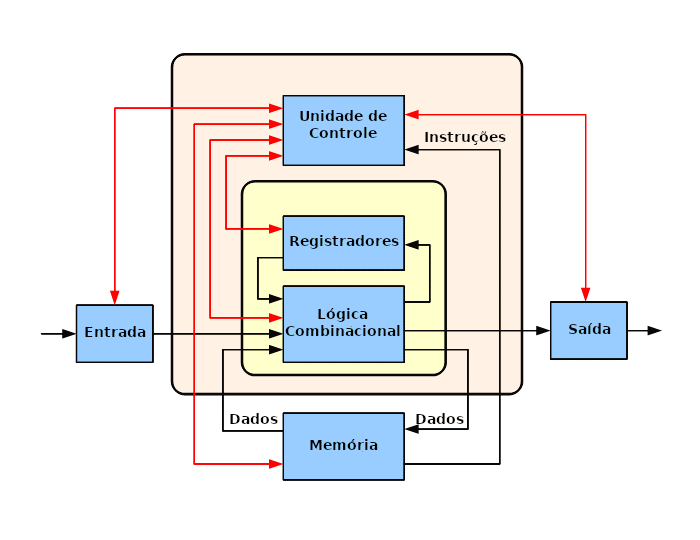
\includegraphics[width=.75\linewidth]
    {../images/ABasicComputer.png}
    \caption[Abstração da arquitetura de um computador]
    {Abstração da arquitetura de um
        computador. Fonte:~\cite{wikimedia2015basiccpu}}\label{fig:cpu_abstraction}
\end{figure}

    \subsection{Arquiteturas \textit{RISC} e \textit{CISC}}
    { Historicamente, as arquiteturas são divididas em \textit{ISAs} \textit{RISC}
        (\textit{Reduced Instruction Set Computer}) e \textit{CISC}
        (\textit{Complex Instruction Set Computer}).  Na atualidade, a principal
        diferença entre elas é que as \textit{ISAs RISC} acessam a memória por
        instruções de \textit{load/store}, enquanto as \textit{CISC} podem acessar
        a memória diretamente em uma instrução de operação lógica ou
        aritmética.~\cite{risc_cisc_wars}
    }

    { Algumas arquiteturas \textit{RISC} notáveis são a \textit{RISC-V}, objeto de
        estudo desse trabalho, a \textit{ARM} e a \textit{MIPS}. Quanto às
        \textit{CISC}, a \textit{x86} e sua extensão de 64 \textit{bits}, a
        \textit{AMD64}, são as mais conhecidas e amplamente utilizadas.
    }

    \subsection{Arquitetura MIPS}
    { Durante seus 36 anos de existência, a \textit{ISA MIPS} (\textit{Microprocessor
        without Interlocked Pipelined Stages}) teve diversas versões produzidas,
        atendendo às demandas de diversos segmentos do mercado. Usado em
        supercomputadores na década de 90 e nos famosos \textit{videogames
        Nintendo 64, PlayStation, PlayStation 2 e PlayStation Portable}, a
        arquitetura atendia a vários segmentos do mercado.
    }

    { A \textit{MIPS32}, uma de suas versões lançada em 1999~\cite{mips32_1999},
        é amplamente utilizada no meio acadêmico, utilizando livros como as
        diversas edições do \textit{Computer Organization and
        Design}~\cite{patterson2014computer} e o clássico
        \textit{See MIPS run}~\cite{sweetman1999see} como livros-texto das
        disciplinas de arquitetura de computadores.
    }

    { Na última década, o uso de processadores \textit{MIPS} têm se limitado a
        sistemas automotivos e roteadores de \textit{internet}~\cite{mips_uses_wiki},
        e a empresa detentora dos direitos da arquitetura anunciou o fim do
        desenvolvimento de novas iterações.~\cite{wave_comp_bankrupt}
    }

    \subsection{Arquitetura ARM}
    { A arquitetura \textit{ARM} (\textit{Advanced RISC Machines}) é considerada
        extremamente eficiente no consumo de energia e possui boa dissipação de
        calor sem comprometer seu desempenho~\cite{arm_facts1988}, e com isso é
        predominante no mercado de \textit{smartphones}~\cite{arm_milestone}.
        Presente também nos \textit{videogames Nintendo 3DS e Nintendo Switch},
        nos \textit{Single Board Computers} (\textit{SBCs}) \textit{Raspberry Pi},
        entre outros dispositivos, a arquitetura tem enorme força em aplicações
        embarcadas.
    }

    { Porém, isso não a impede de atender a outros setores do mercado. Atualmente,
        o supercomputador mais potente do mundo utiliza a arquitetura
        \textit{ARM}.~\cite{arm_super} A \textit{Apple} recentemente lançou seus
        primeiros \textit{notebooks} e \textit{desktops} com seu processador
        \textit{Apple M1}, considerado hoje o processador de computadores pessoais
        com maior eficiência por \textit{watt}.~\cite{arm_m1} O serviço de
        computação em nuvem \textit{Amazon Web Services} (\textit{AWS})
        também oferece máquinas equipadas com seu processador \textit{AWS Graviton}
        para computação geral.
    }

    { A empresa \textit{ARM} opera licenciando o uso do seu conjunto de instruções
        e de projetos de implementação, mas não produz \textit{chips}. A manufatura
        do processador fica a cargo da empresa licenciante, como a \textit{Qualcomm},
        \textit{NXP}, \textit{Samsung} e \textit{Apple}.
    }

    { Por ser uma das arquiteturas prevalentes da atualidade, a \textit{ISA ARM}
        era uma forte candidata para ser utilizada no presente trabalho. Porém,
        a \textit{ISA ARM} não era uma arquitetura aberta, sendo necessário obter
        uma licença para desenvolvimento e distribuição de implementações.
        Atualmente, algumas de suas versões foram parcialmente abertas~\cite{arm_open}.
    }

    \subsection{Arquitetura x86}
    { A \textit{ISA x86}, também conhecida como \textit{IA-32} é uma arquitetura
        \textit{CISC} de 32 \textit{bits} criada em 1985 pela \textit{Intel}
        para uso no seu processador \textit{80386}, renomeado para \textit{i386}.
        Um diferencial da \textit{ISA x86} é que versões mais novas do conjunto
        de instruções mantém a compatibilidade com as versões anteriores.
        Assim, programas desenvolvidos para versões mais antigas continuam
        funcionando em sistemas modernos. Essa característica fez com que
        processadores \textit{x86} dominassem o mercado de computadores pessoais
        e \textit{workstations}.
    }

    { Apesar de criada pela \textit{Intel} para a manufatura de seus próprios
        processadores, a \textit{ISA} foi licenciada para outras empresas como a
        \textit{AMD}.
    }

    \subsection{Arquitetura AMD64}
    { A arquitetura \textit{AMD64} também conhecida como \textit{x86-64} é a
        extensão de 64 \textit{bits} da \textit{IA-32}, criada pela \textit{AMD}
        em 1999. A \textit{Intel} criou sua própria extensão para a \textit{IA-32},
        a \textit{IA-64} da linha de processadores \textit{Itanium}. Porém, a
        extensão criada pela \textit{AMD} teve mais tração e a \textit{Intel}
        também adotou a \textit{AMD64}. A característica de iterações mais novas
        manterem compatibilidade com \textit{softwares} desenvolvidos para versões
        anteriores também faz parte da especificação da arquitetura.
    }

    { Hoje, a maioria predominante dos computadores pessoais modernos,
        \textit{workstations} e servidores utilizam processadores \textit{x86-64}.
    }

\section{A Arquitetura RISC-V}\label{riscv_basic_arch}
{ Conforme descrito na Seção~\ref{intro_riscv}, a \textit{RISC-V} é uma
    arquitetura de especificação aberta e licença livre, o que permite que
    qualquer indivíduo ou entidade produza, distribua e/ou comercialize
    processadores que a utilizem sem haver cobrança de \textit{royalties}.
}

{ A \textit{RISC-V} é uma arquitetura modular, sendo o módulo base de
    operações com inteiros mandatório em qualquer implementação.
    Esse módulo será o \textbf{I} (de \textit{\textbf{I}nteger}) para a
    maioria das implementações. Ele possui 32 registradores, sendo 31 de uso
    geral e um \textit{hardwired} para o valor \texttt{zero}. Mas também existe
    o módulo \textbf{E} (de \textit{\textbf{E}mbedded}) para aplicações embarcadas,
    que possui metade dos registradores presentes nas outras implementações
    (15 de uso geral mais o \texttt{zero}) e é limitado a registradores de
    32 \textit{bits} de largura. As demais extensões são de uso opcional.
}

{ O módulo \textbf{I} pode ser implementado com registradores de 32, 64 ou
    128 \textit{bits} de largura. O módulo com registradores de 128
    \textit{bits} é um planejamento para o futuro quando 64 \textit{bits}
    não forem mais suficientes para o endereçamento de memória do sistema,
    fazendo com que a arquitetura não tenha que ser reprojetada para se
    adequar às novas demandas. Assim, os possíveis conjuntos de instrução
    base são: \textit{RV32I}, \textit{RV32E}, \textit{RV64I} e \textit{RV128I}.
}

{ O \textit{design} do módulo visa reduzir o \textit{hardware} necesário para
    uma implementação mínima, bem como ser um alvo de compilação satisfatório,
    sendo capaz de emular por \textit{software} as extensões \textbf{M}
    (de \textit{\textbf{M}ultiplication and Division}), \textbf{F} (de
    \textit{Single-Precision \textbf{F}loating-Point}) e \textbf{D} (de
    \textit{\textbf{D}ouble-Precision Floating-Point}). Para isso, são
    implementadas instruções de \textit{load/store} para transferir dados
    entre a memória e os registradores, operações lógicas e aritméticas
    entre dados de registradores, instruções para transferência de controle
    (\textit{jumps} e \textit{branches} condicionais) e chamadas de sistema
    (\textit{syscalls}).
}

{ Diferente de outras arquiteturas como a \textit{ARM}, as instruções de
    multiplicação e divisão não fazem parte do conjunto básico, uma vez que
    necessitam de circuito especializado e por isso encarecem o desenvolvimento
    e produção dos processadores.
}

{ A arquitetura foi projetada para aceitar instruções de tamanho variável.
    A codificação do tamanho das instruções é mostrada na
    Figura~\ref{fig:riscv_var_length}. As instruções do módulo \textbf{I}
    seguem o \textit{encoding} de instruções de 32 \textit{bits}. A extensão
    \textbf{C} (de \textit{\textbf{C}ompact}) especifica instruções utilizando
    a codificação de 16 \textit{bits}. As demais extensões previstas pela
    especificação da arquitetura também utilizam a codificação de 32
    \textit{bits}. As codificações para instruções com mais de 32
    \textit{bits} de largura foram projetadas para acomodar necessidades
    futuras e para permitir que projetistas extendam a arquitetura com módulos
    proprietários.
}

\begin{figure}[H]
\centering
    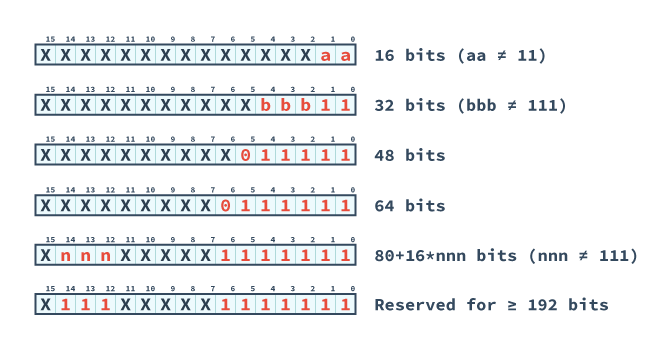
\includegraphics[width=.8\linewidth]{../images/RV_InstructionLength.png}
    \caption{Codificação de instruções de tamanho variável da arquitetura
                \textit{RISC-V}}\label{fig:riscv_var_length}
\end{figure}


    \subsection{Extensão de Registradores de Controle e Estado}
    { A extensão \textbf{Zicsr} implementa o banco de \textit{Control and
        Status Registers} (\textit{CSRs}) e as instruções para acessá-los.
        Esses registradores contemplam um relógio de tempo real (\textit{RTC}),
        contadores de instruções processadas e \textit{ticks} do \textit{clock},
        além de habilitar/desabilitar funcionalidades do processador e checar
        seu estado.
    }

    \subsection{Extensão de Multiplicação e Divisão}
    { As operações aritméticas de multiplicação, divisão e resto de números
        inteiros são implementadas pela extensão \textbf{M}.
    }

    \subsection{Extensões de Ponto Flutuante}
    { A extensão \textbf{F} implementa instruções de ponto flutuante
        \textit{IEEE 754 - 2008} de precisão simples que adiciona
        no processador um banco de 32 registradores de 32 \textit{bits}
        usado para suas operações e um \textit{CSR} para controlar o modo
        de arredondamento e identificar anormalidades na execução de uma
        instrução e.g. divisão por zero.
    }

    { Suas instruções contemplam \textit{load/store} no banco de registradores
        de ponto flutuante, transferência de dados entre os registradores de
        ponto flutuante e os de números inteiros (com ou sem conversão para
        inteiro), operações aritméticas e comparações.
    }

    { A extensão \textbf{D} requer a implementação da extensão \textbf{F} e
        adiciona suporte para operações de ponto flutuante de precisão dupla,
        aumentando a largura do banco de registradores de ponto flutuante
        para 64 \textit{bits}. Há ainda a extensão \textbf{Q} para operações
        de ponto flutuante com precisão quádrupla, que depende da extensão
        \textbf{D} estar implementada e extende a largura do banco de
        registradores de ponto flutuante para 128 \textit{bits}.
    }

    \subsection{Extensões A e Zifencei}
    { A extensão \textbf{A} implementa instruções de acesso atômico a memória,
        enquanto a extensão \textbf{Zifencei} implementa \textit{fencing}
        para escrita e leitura da memória de instruções em um \textit{hart}.
    }

    \subsection{Nomenclatura da implementação}
    { A nomenclatura de um processador \textit{RISC-V} segue a seguinte
        estrutura: as letras \textbf{RV} seguidas da largura do banco de
        registradores (\textbf{32/64}), da letra do módulo base (\textbf{I/E}),
        conforme visto na Seção~\ref{riscv_basic_arch}, e em seguida as outras
        extensões implementadas.
    }

    { As extensões \textbf{M}, \textbf{A}, \textbf{F}, \textbf{D},
        \textbf{Zicsr} e \textbf{Zifencei} utilizadas com o módulo \textbf{I}
        constituem um conjunto considerado um alvo razoável para o
        desenvolvimento de um processador de uso geral. Pela convenção de
        nomenclatura, um processador de 64 \textit{bits} com essa implementação
        se chamaria \textbf{RV64IMAFDZicsr\_Zifencei}. Para uma melhor
        apresentação, o conjunto \textbf{IMAFDZicsr\_Zifencei} pode ser abreviado
        para \textbf{G} (de \textit{\textbf{G}eneral-purpose}). Assim, o
        processador descrito pode ser chaamdo de \textbf{RV64G}.
    }

    \subsection{Outras Extensões}
    { Existem propostas de adição de algumas extensões na especificação da
        \textit{ISA}, como a \textbf{B} para manipulação de \textit{\textbf{B}its}
        e a \textbf{V} para operar \textbf{V}etores, mas ainda não foram
        ratificadas.
    }

    {Há também a possibilidade de se desenvolver extensões próprias. A regra
        de nomenclatura para esse caso é iniciar o nome da extensão com um
        \textbf{X} seguido por um nome alfabético e.g. \textbf{Xhwacha}.
    }

    \subsection{Arquitetura Privilegiada}
    { Para a \textit{ISA RISC-V}, existem quatro níveis de privilégio de acesso,
        sendo eles: o de máquina (nível \textit{bare-metal} que em implementações
        mais simples trata \textit{syscalls}), o de usuário (o nível onde a
        aplicação do usuário é executada), o de supervisor (nível do sistema
        operacional) e o de hipervisor (virtualização).
    }

    { O nível privilegiado de máquina adiciona alguns \textit{CSRs} importantes
        como o \texttt{misa} (\textit{Machine ISA register}), que indica as
        capacidades do processador como largura dos registradores e extensões
        implementadas codificados em \textit{bit fields}, o \texttt{mstatus}
        que controla o estado operacional do \textit{hart} como a habilitação
        de interrupções, o \texttt{mtvec} que contém o endereço de memória
        do tratamento de \textit{traps}, o \texttt{mepc} que guarda o endereço
        de memória onde uma instrução causou uma exceção e o \texttt{mcause}
        que indica a causa da exceção.
    }

    \subsection{Formatos de Instruções}
    { As instruções da arquitetura podem ser separadas em subgrupos de acordo com
        os operadores necessários para o processador interpretá-la. A
        Figura~\ref{fig:riscv_formats} apresenta os formatos das instruções do
        módulo I da \textit{ISA RISC-V}, e, para efeitos de comparação, a
        Figura~\ref{fig:mips_formats} mostra os formatos de instruções equivalentes
        na arquitetura \textit{MIPS32}.
    }

    { Apesar dos formatos das instruções da \textit{RISC-V} serem mais
        complicados que os da \textit{MIPS32} do ponto de vista de um
        humano, para uma máquina eles são muito mais eficientes. Os campos
        do \texttt{opcode}, do \texttt{funct3}, dos registradores \texttt{rs1},
        \texttt{rs2} e \texttt{rd}, e alguns bits dos imediatos \texttt{imm}
        sempre se encontram na mesma posição na instrução. Isso reduz a
        complexidade dos multiplexadores de geração de imediatos e da lógica
        de decodificação da instrução. Além disso, por utilizar imediatos de
        12 \textit{bits} (ou 20 no caso das instruções do tipo \textbf{U})
        em vez de imediatos de 16 \textit{bits} (ou 28 nas instruções do
        tipo \textbf{J}), a \textit{ISA RISC-V} possui mais \textit{bits}
        disponíveis para codificar mais instruções.
    }

    \begin{figure}[H]
    \centering
        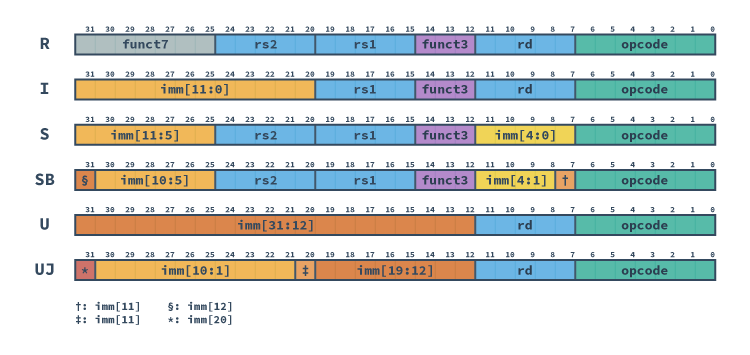
\includegraphics[width=.9\linewidth]{../images/RV_Formats.png}
        \caption{Formatos de Instruções da \textit{ISA RISC-V}}\label{fig:riscv_formats}
    \end{figure}

    \begin{figure}[H]
    \centering
        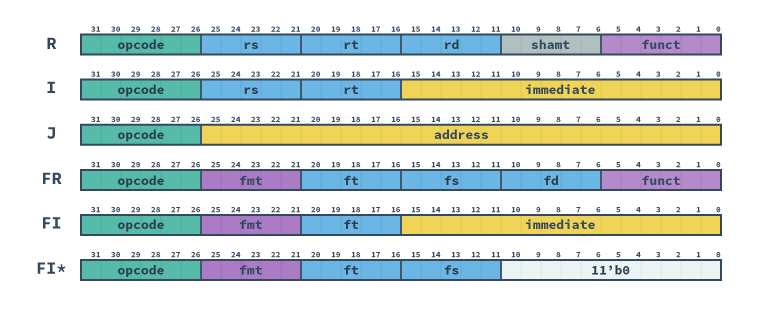
\includegraphics[width=.8\linewidth]{../images/MIPS_Formats.png}
        \caption{Formatos de Instruções da \textit{ISA MIPS32}}\label{fig:mips_formats}
    \end{figure}

    \subsection{Formatos de Imediatos}
    { Os imediatos são operandos descritos na própria instrução em vez de
        estarem contidos em um registrador. Como os operandos necessitam ter
        a mesma largura que o banco de registradores, algumas regras são
        utilizadas para gerar os imediatos. As figuras a seguir mostram a
        formação de cada tipo de imediato dos formatos das instruções
        apresentadas na Figura~\ref{fig:riscv_formats}.
    }

    \begin{figure}[H]
    \centering
        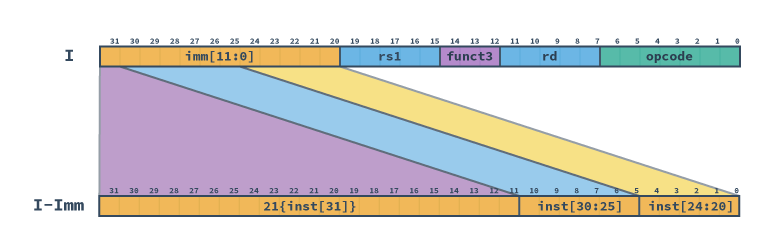
\includegraphics[width=.9\linewidth]{../images/RV_I_Imm.png}
        \caption{Formação do Imediato de tipo I}\label{fig:riscv_i_imm}
    \end{figure}

    \begin{figure}[H]
    \centering
        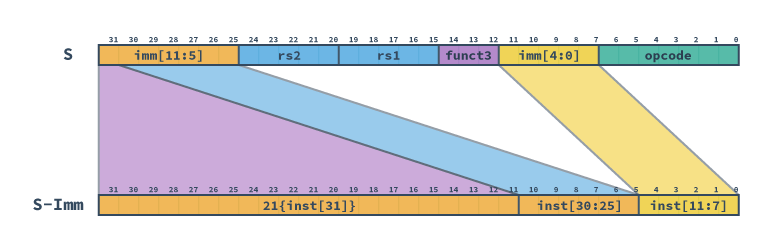
\includegraphics[width=.9\linewidth]{../images/RV_S_Imm.png}
        \caption{Formação do Imediato de tipo S}\label{fig:riscv_s_imm}
    \end{figure}

    \begin{figure}[H]
    \centering
        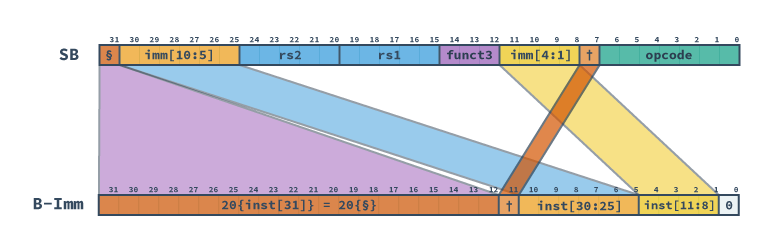
\includegraphics[width=.9\linewidth]{../images/RV_B_Imm.png}
        \caption{Formação do Imediato de tipo B}\label{fig:riscv_b_imm}
    \end{figure}

    \begin{figure}[H]
    \centering
        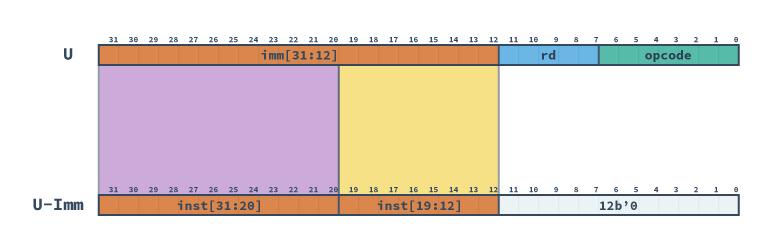
\includegraphics[width=.9\linewidth]{../images/RV_U_Imm.png}
        \caption{Formação do Imediato de tipo U}\label{fig:riscv_u_imm}
    \end{figure}

    \begin{figure}[H]
    \centering
        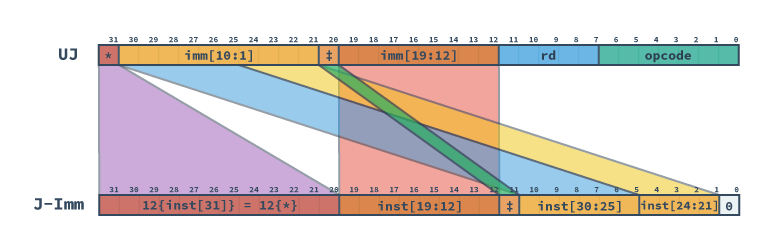
\includegraphics[width=.9\linewidth]{../images/RV_J_Imm.png}
        \caption{Formação do Imediato de tipo J}\label{fig:riscv_j_imm}
    \end{figure}


\section{\textit{IDE RARS}}\label{rars_cap2}
{ O Ambiente Integrado de Desenvolvimento (\textit{IDE}) \textit{RARS}
    (\textit{RISC-V Assembler and Runtime Simulator}) é um \textit{software
    open source}~\cite{rars_git} utilizado para desenvolver, montar, simular e
    exportar código em \textit{assembly RISC-V}. O projeto é um \textit{fork}
    do \textit{MARS} (\textit{MIPS Assembler and Runtime Simulator}), outro
    \textit{software open source}~\cite{mars_site} muito utilizado em cursos
    de arquitetura de computadores ministrados em \textit{MIPS32}.
}
\begin{figure}[H]
\centering
    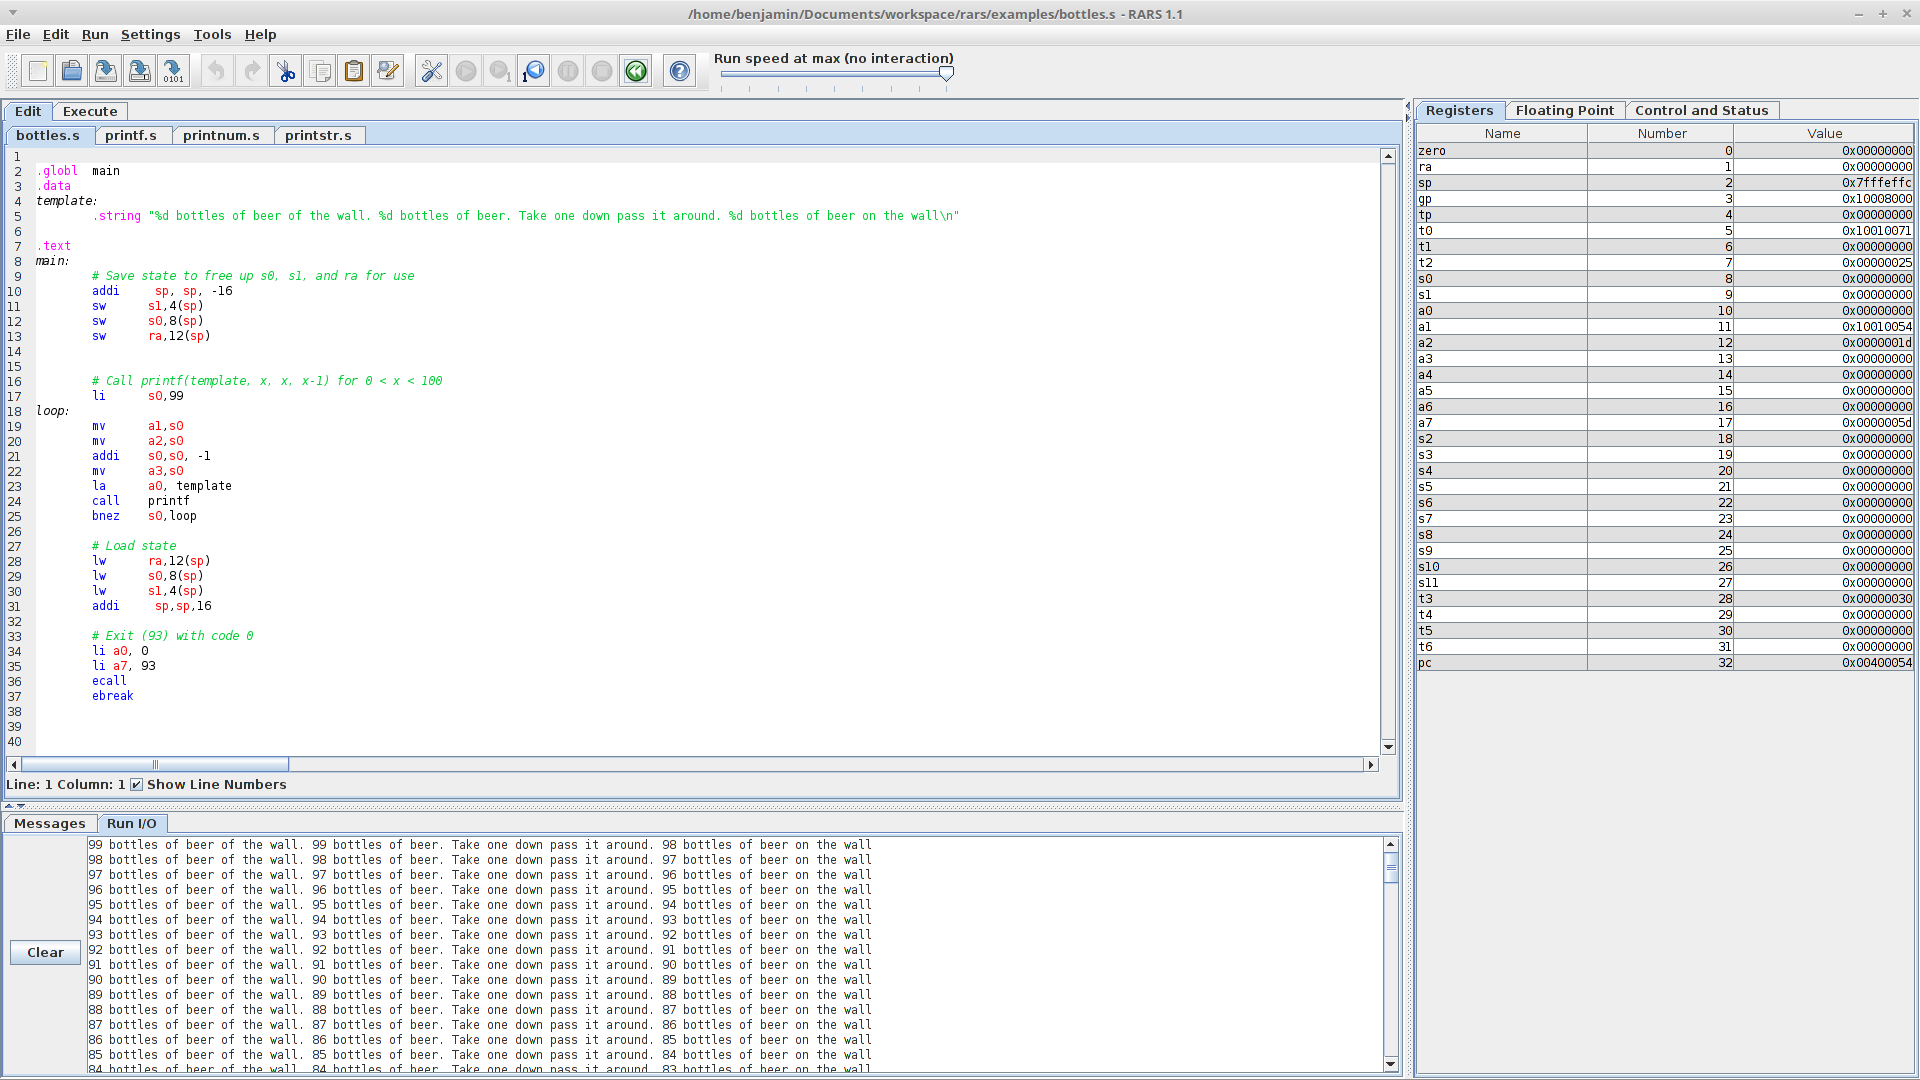
\includegraphics[width=.9\linewidth]{../images/rars.png}
    \caption{\textit{IDE RARS}}\label{fig:rars}
\end{figure}

{ O \textit{RARS} é compatível com as \textit{ISAs} \textbf{RV32IMFD} e
    \textbf{RV64IMFD} com suporte a interrupções e implementa parcialmente a
    extensão \textbf{Zicsr}. Também tem suporte a \textit{syscalls}. Possui
    também um guia de programação em \textit{assembly RISC-V} e pode ser
    utilizado como referência de instruções e pseudo-instruções.
}

{ Com sua função de simulador, permite executar o código instrução por instrução,
    mostrando as modificações nos bancos de registradores e na memória. Além
    disso, permite exportar o programa montado no formato \textit{.mif} para
    uso na inicialização de memória de \textit{FPGAs}.
}


\section{Microarquiteturas}
{ Enquanto o campo de arquitetura de computadores explora a especificação dos
    conjuntos de instruções, a organização de computadores trata da forma com que
    as especificações são implementadas. Os padrões de implementação de
    \textit{ISAs} são chamados de microarquiteturas, e esses padrões podem ser
    combinados para produzir soluções mais complexas.
}

{ Processadores são circuitos elétricos, e podem ser descritos por diagramas.
    Nesses diagramas, o caminho de dados (\textit{datapath}) representa a
    conexão feita entre blocos lógicos por barramentos onde os sinais a serem
    processados trafegam. A unidade de controle é responsável por interpretar as
    instruções recebidas e comandar os blocos lógicos para executar o comando.
    Os blocos lógicos são as Unidades de Lógica e Aritmética (ULA, ou
    \textit{ALU} em inglês), bancos de registradores (\textit{regfiles})
    multiplexadores e blocos de memória.
}

    \subsection{Uniciclo}
    { Processadores uniciclo são implementados de forma com que cada instrução
        seja recuperada (\textit{fetch}), decodificada (\textit{decode}),
        executada e finalizada (\textit{retire}) durante um único \textit{tick}
        do \textit{clock}. Para isso, a unidade de controle deve conter somente
        lógica combinacional e a frequência de operação do \textit{clock} deve
        ser projetada para o pior caso, ou seja, a instrução que leva mais tempo
        entre seu \textit{fetching} e seu \textit{retiring}.
    }

    { A implementação da microarquitetura uniciclo é uma das mais mais simples
        de se fazer, mas o processador resultante apresenta baixa frequência de
        processamento. Para \textit{workloads} que utilizam muitas instruções
        complexas, seu desempenho pode ser parecido ou até melhor que implementações
        mais elaboradas, mas se a maioria da carga de processamento for de
        instruções rápidas, o uniciclo sofre uma penalidade por ficar ocioso
        durante parte do seu ciclo.
    }

    \subsection{Multiciclo}
    { A microarquitetura multiciclo também é conhecida como implementação por
        microcódigo. As instruções são ``quebradas'' em etapas menores, como
        o acesso à memória, a leitura do banco de registradores, a seleção de um
        sinal multiplexado, a realização de uma operação lógica ou aritmética,
        dentre outras possibilidades. A unidade de controle é implementada por
        lógica sequencial como uma máquina de estados finitos, e a frequência
        máxima de operação é limitada pela etapa mais lenta da máquina de estados.
    }

    { Como a quantidade de estados que uma instrução deve passar entre seu
        \textit{fetching} e \textit{retiring} depende de sua complexidade e de
        como a máquina de estados foi projetada, a frequência do \textit{clock}
        costuma ser mais alta que de uma implementação uniciclo, mas isso não
        significa que seu desempenho será melhor, pois o desempenho também depende
        do \textit{workload}. Se a maioria das instruções executadas precisa
        passar por diversos estados para serem completadas, o somatório de ciclos
        menores pode resultar em um intervalo de tempo maior que o do ciclo único.
    }

    \subsection{\textit{Pipeline}}\label{cap2_fwd_hzd}
    { Uma implementação \textit{pipeline} consiste em inserir registradores entre
        os blocos lógicos do \textit{datapath}, o dividindo em etapas. O objetivo
        é ser capaz de processar mais de uma instrução por vez. A
        Figura~\ref{fig:pipe_generic} mostra um \textit{pipeline} genérico de
        quatro estágios. O processo inicia com o \textit{fetching} de uma instrução
        no primeiro ciclo do \textit{clock}. No segundo ciclo do \textit{clock},
        a primeira instrução passa para o estágio de \textit{decode} e uma nova
        instrução entra no primeiro estágio do \textit{pipeline}. No terceiro
        \textit{tick}, a primeira instrução está no terceiro estágio, a segunda
        no segundo estágio e a terceira no primeiro estágio. No quarto ciclo,
        a primeira instrução está no quarto estágio, a segunda instrução no
        terceiro estágio, a terceira instrução no segundo estágio e a quarta
        instrução acaba de entrar no \textit{pipeline}. No ciclo seguinte, a
        primeira instrução é finalizada, as outras três instruções passam para
        o estágio seguinte e uma nova instrução entra no primeiro estágio do
        \textit{pipeline}.
    }

    \begin{figure}[H]
    \centering
        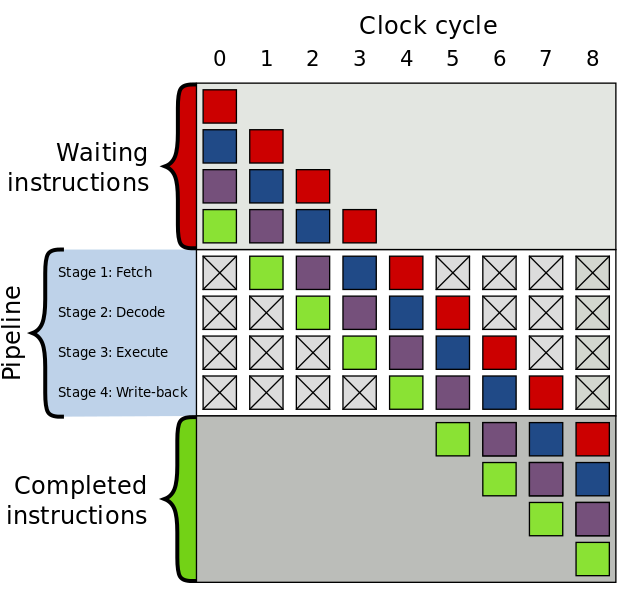
\includegraphics[width=.65\linewidth]{../images/pipeline_4_stage.png}
        \caption[\textit{Pipeline} genérico com 4 estágios]{\textit{Pipeline}
            genérico com 4 estágios. \quad Fonte:~\cite{pipe_generic}}\label{fig:pipe_generic}
    \end{figure}

    { A frequência do \textit{clock} é limitada pelo estágio mais lento. O objetivo
        é manter o \textit{pipeline} com todos os seus estágios preenchidos, e
        assim, a cada \textit{tick}, uma instrução é completada, sendo uma
        implementação com ótimo desempenho. Porém, é comum que uma instrução
        precise do resultado de outra instrução que ainda não foi finalizada.
    }

    { Uma solução simples porém ineficiente para o problema é limpar os estágios
        anteriores, inserindo \texttt{nop}s (instruções que não realizam nenhuma
        tarefa) até que o resultado esteja disponível e voltar a preencher o
        \textit{pipeline}. Uma solução mais robusta seria implementar uma
        unidade de identificação e tratamento de \textit{forwards} e \textit{hazards}.
        \textit{Forwards} ocorrem quando a instrução anterior ainda não finalizou,
        mas seu resultado já está disponível em algum estágio do \textit{pipeline}
        e o valor pode ser injetado na etapa que precisa dele. Já os \textit{hazards}
        são situações onde o \textit{forward} não é possível e \texttt{nop}s
        precisam ser inseridos.
    }


\section{Representação de \textit{Hardware}}
{ Existem diversas maneiras de representar circuitos eletrônicos. Na programação
    visual, as entradas e saídas dos blocos funcionais são conectados de forma
    gráfica, montando um diagrama do circuito. Já as linguagens de descrição de
    \textit{hardware} (\textit{HDLs}) como o \textit{Verilog} e o \textit{VHDL}
    permitem uma descrição precisa da estrutura e comportamento dos circuitos.
    Outra forma de representação utiliza a síntese de alto nível (\textit{High-Level Synthesis}),
    onde se desenvolve um algoritmo em linguagens como \textit{C++} ou \textit{MATLAB},
    que será ``traduzido'' para um circuito eletrônico.
}

{ Essas reprentações permitem a geração de \textit{netlists} utilizadas para
    simular o projeto, sintetizá-lo em \textit{FPGAs} ou fazer o \textit{tapeout}
    para produção de \textit{chips}.
}

    \subsection{\textit{Verilog}}
    { \textit{Verilog} é uma \textit{HDL} comumente utilizada no projeto \textit{RTL}
        de circuitos lógicos. Módulos escritos em \textit{Verilog} descrevem seus
        sinais de entrada e saída como parâmetros para a conexão com outros módulos.
        As suas principais ``variáveis'' são \textit{wires} (fios que conectam
        um sinal a outro) e \textit{regs} (registradores ou \textit{drivers} de
        sinal). A lógica do módulo pode ser implementada por \textit{assignments}
        (a conexão de um fio a um registrador ou um \textit{driver}) ou por
        blocos de lógica sequencial ou combinacional, usando operadores blocantes
        (\texttt{=}) ou não-blocantes (\texttt{<=}).
    }

    { Para quem está acostumado com linguagens imperativas como o \textit{C},
        há uma barreira inicial para entender que o código não é executado linha
        por linha, mas sim de maneira concorrente, e que a escolha entre operadores
        blocantes e não-blocantes afeta a forma com que os sinais são propagados
        no circuito.
    }

    { A sintaxe do \textit{Verilog} é menos verbosa que a do \textit{VHDL}, que
        é fortemente tipada. Enquanto a verificação formal de \textit{designs}
        em \textit{VHDL} é um processo mais natural, o \textit{Verilog} possui
        uma curva de aprendizado menor, sendo ideal para o primeiro contato com
        linguagens de descrição de \textit{hardware}.
    }

    \subsection{Análise e Síntese}
    { O processo de análise de representações de \textit{hardware} verifica a
        sintaxe da representação, identificando estruturas inválidas, sinais não
        conectados e possíveis erros semânticos que farão com que a \textit{netlist}
        não possa ser gerada ou não se comporte conforme o esperado.
    }

    { Já a síntese é o processo de transformar a estrutura analisada em uma
        \textit{netlist}, estrutura que contém a lista de componentes eletrônicos
        do \textit{design} e a descrição de como eles se conectam.
    }

    \subsection{\textit{Fitting} e \textit{Timing Analyzer}}
    { O \textit{fitting} é o processo de criar as rotas de conexão da \textit{netlist}.
        O \textit{design} é mapeado para a plataforma onde será implementado.
        Já o \textit{timing analyzer} define restrições de temporização entre
        elementos do circuito que o \textit{fitter} tenta respeitar. O
        \textit{fitter} itera diversas vezes o posicionamento e roteamento dos
        componentes até gerar o resultado final.
    }

    { Com a \textit{netlist} roteada, o \textit{Timing Analyzer} é executado
        novamente, testa se o \textit{fitter} conseguiu atender às restrições e
        gera um relatório. Caso alguma rstrição essencial não for respeitada,
        o \textit{Fitter} pode ser novamente executado com opções diferentes que
        impactarão outras características do circuito final, como quantidade de
        componentes e consumo energético.
    }

    { Pode ser necessário reimplementar a
        representação do \textit{hardware} para que todos os requisitos de projeto
        sejam atendidos.
    }


\section{Field Programmable Gate Arrays}
{ \textit{Field Programmable Gate Arrays} (\textit{FPGAs}) são circuitos
    integrados que permitem o desenvolvimento de circuitos lógicos
    reconfiguráveis. Por serem reprogramáveis, as \textit{FPGAs} geram uma
    grande economia em tempo de desenvolvimento e em custos como os de
    prototipagem, validação e manufatura do projeto em relação aos circuitos de
    aplicações específicas, os \textit{ASICs}, e aos projetos
    \textit{full-custom}. As \textit{FPGAs} podem ser tanto o passo
    intermediário no projeto de um \textit{ASIC} ou \textit{full-custom} quanto
    o meio final do projeto quando a reconfigurabilidade e os preços muito mais
    acessíveis forem fatores importantes.
}

{ Cada fabricante de \textit{FPGAs} possui seu \textit{software} de
    desenvolvimento, ou \textit{SDKs}. A indústria de \textit{hardware} é
    extremamente protecionista com sua propriedade intelectual (tanto que os
    \textit{designs} de módulos ou circuitos completos são chamados de \textit{IPs},
    termo derivado de \textit{\textbf{I}ntellectual \textbf{P}roperty}), sendo
    a maioria dessas ferramentas de código proprietário. Para a Intel Altera,
    essa plataforma é o Quartus Prime.
}

{ \textit{FPGAs} mais modernas possuem, além do arranjo de portas lógicas,
    blocos de memória, \textit{Phase-Locked Loops} (\textit{PLLs}),
    \textit{Digital Signal Processors} (\textit{DSPs}) e \textit{System on
    Chips} (\textit{SoCs}). Os blocos de memória internos funcionam como a memória
    \textit{cache} de um microprocessador, armazenando os dados próximo ao seu
    local de processamento para diminuir a latência. Os \textit{PLLs} permitem criar
    sinais de \textit{clock} com diversas frequências a partir de um relógio de
    referência, e podem ser reconfigurados a tempo de execução. \textit{DSPs}
    são responsáveis pelo processamento de sinais analógicos discretizados, e
    podem ser utilizados como multiplicadores de baixa latência. Já os
    \textit{SoCs} são microprocessadores como os ARM presentes em celulares,
    e são capazes de executar sistemas operacionais como o Linux.
}

{ Além de disponíveis na forma de \textit{chips} para a integração com placas
    de circuito impresso customizadas (\textit{PCBs}), as \textit{FPGAs} possuem
    \textit{kits} de desenvolvimento com diversos periféricos para auxiliar no
    processo de criação de soluções. Esses \textit{kits} são a principal ferramenta
    de aprendizagem no universo dos circuitos reconfiguráveis. No Laboratório de
    Informática da UnB, as placas \textit{terasIC DE1-SoC} com a \textit{FPGA
    Intel Cyclone V SoC} estão disponíveis para os alunos de OAC desenvolverem
    seus projetos.
}

    \subsection{Arquitetura Generalizada de uma FPGA}
    { De forma genérica, uma \textit{FPGA} possui blocos lógicos, chaves de
        interconexão, blocos de conexão direta e portas de entrada e saída,
        conforme apresentado na Figura~\ref{fig:fpga_general_arch}.
    }

    \begin{figure}[H]
    \centering
    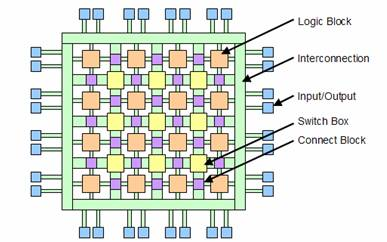
\includegraphics[width=.7\linewidth]
        {../images/fpga_architecture_abstraction_-_olin_college.jpg}
        \caption[Abstração da arquitetura de uma FPGA]
            {Abstração da arquitetura de uma FPGA.\quad Fonte:~\cite{fpga_arch_abstraction}}
        \label{fig:fpga_general_arch}
    \end{figure}

    { Os blocos lógicos possuem \textit{lookup tables}, registradores, somadores
        e multiplexadores. É neles que a lógica reconfigurável é implementada.
        Já as chaves de interconexão são responsáveis por conectar os diversos
        blocos lógicos da \textit{FPGA}. A Figura~\ref{fig:fpga_switch_box} exemplifica
        como é feito o roteamento da malha de interconexão. Os blocos de conexão
        direta são um tipo especial de chave de interconexão, e sua função é ligar
        blocos lógicos adjacentes. Por fim, as portas de entrada e saída conectam
        a \textit{FPGA} ao ``mundo externo'' e.g. \textit{drivers} de áudio e vídeo.
    }

    \begin{figure}[H]
    \centering
    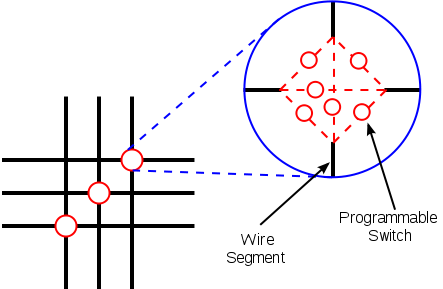
\includegraphics[width=.5\linewidth]
        {../images/switch_box_wikimedia.png}
        \caption[Funcionamento da chave de interconexão]
            {Funcionamento da chave de interconexão.\quad Fonte:~\cite{fpga_switch_box}}
        \label{fig:fpga_switch_box}
    \end{figure}


    \subsection{Arquitetura da FPGA Cyclone V SoC}
    { A Figura~\ref{fig:cyclone_v_arch} apresenta a arquitetura da
        \textit{FPGA Cyclone V SoC}. O \textit{chip} possui um processador
        \textit{ARM} integrado, blocos de memória embutidos, \textit{DSPs} para
        acelerar operações como multiplicação de números ou processamento de
        sinais genéricos, diversos pinos para integrar o \textit{chip} a
        um projeto de circuito mais complexo, \textit{PLLs} para gerar diversos
        sinais de \textit{clock}, entre outras funcionalidades.
    }

    \begin{figure}[H]
    \centering
    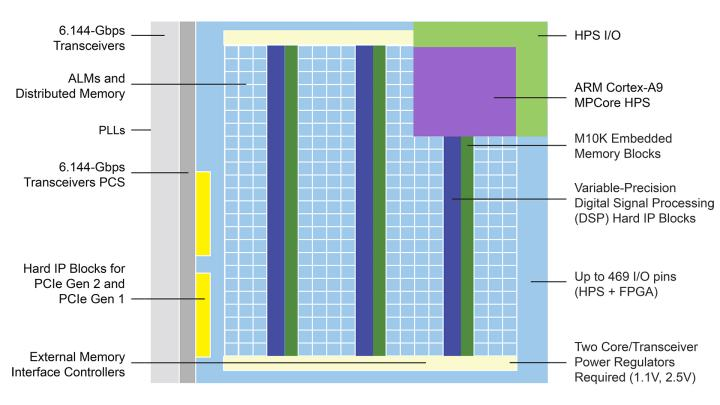
\includegraphics[width=1\linewidth]
        {../images/altera_cyclone_v_soc_architectural_downscale.jpg}
        \caption[Arquitetura da FPGA Intel Cyclone V SoC]
            {Arquitetura da \textit{FPGA Altera Cyclone V SoC}.\quad Fonte:~\cite{cyclone_v_soc}}
        \label{fig:cyclone_v_arch}
    \end{figure}

        \subsubsection{Adaptative Logic Modules}
        { Os blocos lógicos, como mostrados na abstração da Figura~\ref{fig:fpga_general_arch}
            são implementados na \textit{FPGA Cyclone V SoC} como
            \textit{Adaptative Logic Modules}, conforme a Figura~\ref{fig:fpga_alm}.
            Como os \textit{ALMs} são blocos genéricos, há um \textit{trade-off}
            entre configurabilidade e performance.
        }

        \begin{figure}[H]
        \centering
        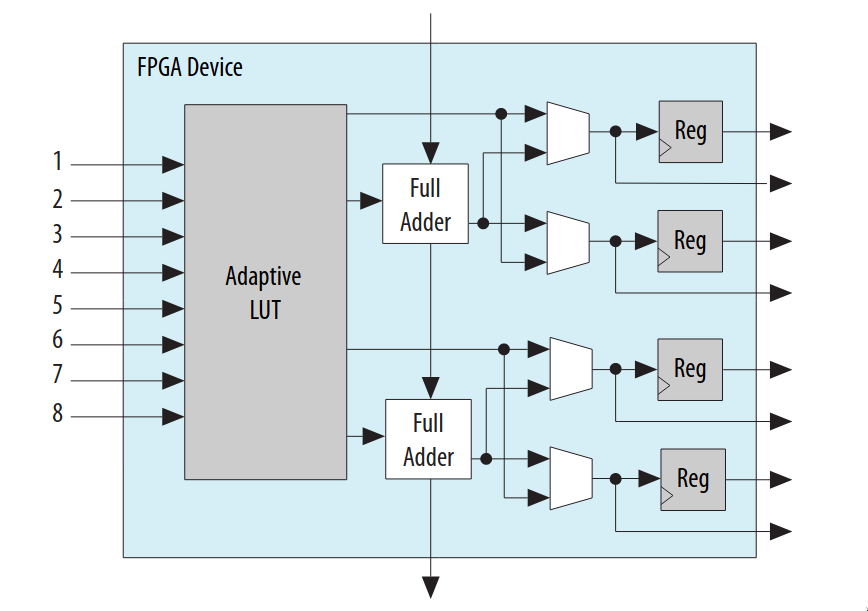
\includegraphics[width=.7\linewidth]
            {../images/intel_alm_high_level.png}
            \caption[Diagrama de blocos de um ALM]
                {Diagrama de blocos de um ALM.\quad Fonte:~\cite{cyclone_alm}}
            \label{fig:fpga_alm}
        \end{figure}


        \subsubsection{Embedded Memory Blocks}
        { Como mostrado na Figura~\ref{fig:cyclone_v_arch}, existem blocos de
            memória embutidos na \textit{FPGA}. Esses blocos são o equivalente
            a uma memória \textit{cache L1}, sendo a camada de memória mais próxima
            dos registradores. Para utilizá-los no \textit{design} do circuito,
            blocos do \textit{IP} de memória são configurados e instanciados
            pelo programa de desenvolvimento para gerar um módulo integrável no
            resto do \textit{design}.
        }

        { As placas de desenvolvimento podem possuir outros tipos de memória,
            como as \textit{SRAM} e \textit{DRAM}. Apesar de possuírem capacidade
            de armazenamento bem maiores que os blocos embutidos, seus
            módulos controladores são mais complexos e apresentam latência maior
            para leitura e escrita de dados. Para seu uso eficiente, é necessário
            implementar camadas de \textit{caching} para que as operações de
            \textit{input} e \textit{output} (\textit{IO}) não se tornem um
            gargalo que comprometa o resto do \textit{design}.
        }


\section{Estado da Arte dos processadores RISC-V}
{ Por alguns anos, processadores com arquitetura \textit{RISC-V} só podiam
    ser utilizados por meio de emuladores como o \textit{qemu}~\cite{qemu_riscv}
    ou em \textit{FPGAs}. Diversos \textit{soft-cores} \textit{open source},
    tanto experimentais (como o desenvolvido neste trabalho) quanto de alto
    desempenho podem ser encontrados na \textit{internet} e utilizados por
    qualquer pessoa interessada. Um dos processadores alto desempenho disponíveis
    é o \textit{BOOM}~\cite{boom_berkeley}, processador com execução
    \textit{Out of Order} desenvolvido na universidade americana \textit{UC Berkeley}
    pelo mesmo departamento onde surgiu a arquitetura \textit{RISC-V}, o
    \textit{Berkeley Architecture Research}~\cite{berkeley_bar}. O processador
    pode ser sintetizado em instâncias \textit{EC2 F1} da
    \textit{AWS}~\cite{boom_aws}, eliminando a necessidade de possuir uma
    \textit{FPGA} de alto desempenho para usufruir do projeto.
}

{ Outro projeto \textit{open source} notável é o \textit{Shakti}~\cite{shakti},
    ecossistema desenvolvido na universidade indiana \textit{IIT-Madras} com
    diversas implementações para os mais diversos usos, que variam desde
    microcontroladores de 32 \textit{bits}, superescalares de 64 \textit{bits}
    para aplicação em \textit{desktops} e servidores até processadores de alta
    performance com mais de 32 \textit{cores}~\cite{shakti_types}.
}

{ Porém, a presença apenas de \textit{soft-cores} limita as possíveis aplicações
    da arquitetura. Algumas fabricantes já divulgaram planos para começar a usar
    microcontroladores com a arquitetura em seus produtos, como é o caso dos
    controladores de discos rígidos e \textit{SSDs} da
    \textit{Western Digital}~\cite{western_riscv} e da Nvidia como o substituto
    dos controladores \textit{Falcon} de suas placas de vídeo~\cite{nvidia_riscv}.
    Ainda não se sabe se as empresas já utilizam os controladores em seus
    \textit{hardwares}, se a adoção ainda está em fase de projeto ou se a ideia
    foi abandonada.
}

{ Porém, começam a surgir no mercado microcontroladores e \textit{Single
    Board Computers (SBCs)} com preços acessíveis. Placas como a linha
    \textit{Sipeed} da \textit{Seed} se equiparam aos \textit{MCUs
    ESP32}~\cite{hackaday_sipeed}, e outras como a \textit{SiFive HiFive1}
    se assemelham aos \textit{arduinos}~\cite{hifive_arduino}.
}

{ Há uma expectativa de \textit{SBCs} mais robustos, capazes de rodar um
    sistema operacional de uso geral, como um \textit{Raspberry Pi}. Existem
    alguns pré-lançamentos de placas para atender essa demanda, como a
    \textit{SiFive HiFive Unmatched}~\cite{hifive_unmatched} e a
    \textit{BeagleV}~\cite{beaglev}.
}

{ A empresa \textit{SiFive}, liderada pelos criadores da arquitetura, produzirá
    em parceria com a \textit{TSMC (Taiwan Semiconductor Manufacturing Company)}
    o primeiro processador \textit{RISC-V} de 32 \textit{bits} em tecnologia
    de 5nm~\cite{sifive_tsmc}. A \textit{TSMC} é a \textit{foundry} líder em
    manufatura de circuitos integrados no mundo.
}

{ Atualmente, compilar códigos em \textit{C/C++} para \textit{targets RISC-V}
    não envolve mais a instalação de \textit{toolchains} complicadas e frágeis.
    Tanto o \textit{gcc}~\cite{gcc_riscv} quanto o \textit{clang}~\cite{clang_riscv}
    já oferecem suporte para o \textit{RISC-V}, eliminando assim uma barreira
    para a adoção da arquitetura.
}

{ Uma outra característica essencial para o uso do \textit{RISC-V} em sistemas
    de uso geral é a existência de sistemas operacionais que funcionem na
    plataforma. Desde a versão 4.15, o \textit{kernel} do \textit{linux}
    oferece suporte para a arquitetura~\cite{linux_kernel}. \textit{Distros}
    como \textit{Fedora}~\cite{fedora_experimental},
    e \textit{Alpine}~\cite{alpine_experimental} já possuem suporte experimental.
    A chinesa \textit{Alibaba} fez o \textit{port} do \textit{OS Android}
    para um de seus \textit{SoCs RISC-V}~\cite{alibaba_android}. Alguns
    ecossistemas mais robustos possuem \textit{ports} completos, como é o
    caso do \textit{Haiku-OS}~\cite{haiku_riscv} e do \textit{microkernel
    seL4}~\cite{sel4_riscv}, possibilitando o uso em ambientes industriais
    e áreas que exigem maior robustez do sistema operacional.
}

{ Uma das surpresas na adoção da arquitetura \textit{RISC-V} nos seus
    \textit{designs} veio da \textit{MIPS Technologies}, detentora das
    patentes das arquiteturas \textit{MIPS}. Em 2013, a empresa foi adquirida
    pela \textit{Imagination Technologies}~\cite{imagination_technologies_acq},
    e lançou alguns \textit{development kits} voltados a visão computacional
    e microcontroladores, mas não conseguiu dar tração aos projetos.
    Em 2017 a companhia foi novamente vendida para a \textit{Tailwood
    Venture Capital}~\cite{tailwood_acq}, que tentou capitalizar em cima dos
    \textit{royalties} da arquitetura. Porém, em 2018 a companhia foi vendida
    novamente para a \textit{Wave Computing}~\cite{wave_comp_acq}, companhia
    voltada para aplicações de inteligência artificial. Em 2020, a
    \textit{Wave Computing} declara falência~\cite{wave_comp_bankrupt},
    demitindo todos os seus funcionários. Em março desse ano, a empresa
    conseguiu se recuperar da falência, mudou o nome da companhia para
    \textit{MIPS} e anunciou que seus novos \textit{designs} serão baseados
    na arquitetura \textit{RISC-V}~\cite{mips_reborn}. Atualmente, a empresa
    \textit{MIPS} integra a \textit{RISC-V Foundation} como Membro Estratégico.
}


\section{Observações finais da Revisão Teórica}
{ O capítulo abordou os conceitos que formam o alicerce do trabalho. O capítulo
    seguinte apresentará a proposta do projeto, descrevendo sua implementação
    e documentando o processo de execução e modificação do produto final a fim
    de permitir sua utilização futura.
}


\chapter{Sistema Proposto}\label{cap3_proposta}

{ O sistema proposto consiste em um \textit{soft-core} da \textit{ISA RISC-V}
    de 32 \textit{bits} com as extensões \textbf{I}, \textbf{M} e \textbf{F},
    podendo ser sintetizado nas versões \textbf{RV32I}, \textbf{RV32IM} ou
    \textbf{RV32IMF}. A extensão \textbf{Zicsr} com os Registradores de Controle
    e Estado (\textit{CSR}) é parcialmente implementada em todas as três
    configurações. Chamadas de sistema (\textit{syscalls}) também são implementadas.
}

{ Cada uma das combinações da \textit{ISA} pode ser realizada em três
    microarquiteturas diferentes: unicicilo, multiciclo ou \textit{pipeline} de
    cinco estágios. Assim, o processador pode ser sintetizado em nove
    combinações diferentes.
}

{ O projeto utiliza a placa de desenvolvimento \textit{terasIC DE1-SoC} contendo
    diversos periféricos e um \textit{SoC Intel Altera Cyclone-V}. A maioria dos
    periféricos presentes na plataforma tem controladores implementados com
    Entradas e Saídas Mapeadas em Memória (\textit{MMIO}) para que o
    \textit{soft-core} possa utilizá-los. A síntese dos controladores dos
    periféricos, como a saída de vídeo, entrada de teclado e barramento
    \textit{RS-232} é opcional.
}

\section{Organização do projeto}
    { O projeto é organizado seguindo o seguinte arranjo de pastas:
    }
\begin{verbatim}
    ┌─ core                     (arquivos que implementam o soft-core)
    │  ├─ clock                 (arquivos de interface e controle de sinais
    │  │                            de clock do processador)
    │  ├─ memory                (arquivos de interface/controle de memória)
    │  ├─ misc                  (módulos como somador e multiplexador de
    │  │                            largura definidas por parâmetros)
    │  ├─ peripherals           (interfaces e controladores para os
    │  │                            periféricos da FPGA)
    │  ├─ risc_v                (projeto do processador RISC-V)
    │  │  ├─ CPU.v              (arquivo top-level do processador)
    │  │  ├─ Control_*.v        (módulos de controle de cada microarquitetura)
    │  │  ├─ Datapath_*.v       (módulos do caminho de dados de cada µarch)
    │  │  └─ ...                (demais módulos do processador)
    │  ├─ config.v              (arquivo de configuração de versão do
    │  │                            processador a implementar, seus
    │  │                            periféricos e endereçamento de memória
    │  │                            das interfaces MMIO)
    │  ├─ default_data.mif      (arquivo de inicialização de memória de
    │  │                            dados usado na síntese do projeto)
    │  ├─ default_framebuffer.mif   (arquivo de inicialização de memória de
    │  │                                vídeo usada na síntese do projeto)
    │  ├─ default_text.mif      (arquivo de inicialização de memória de
    │  │                            texto usado na síntese do projeto)
    │  ├─ fpga_top.sdc          (restrições desejadas de temporização do
    │  │                            sistema sintetizado)
    │  └─ fpga_top.v            (interface verilog entre o soft-core e a
    │                               placa de desenvolvimento)
    ├─ doc                      (documentação e guias do projeto)
    ├─ project                  (arquivos de projeto do Quartus)
    │  ├─ de1_soc
    │  │  ├─ db                 (arquivos de saída intermediários do
    │  │  │                         Quartus; pasta ignorada pelo git)
    │  │  ├─ incremental_db     (arquivos de saída intermediários do
    │  │  │                         Quartus; pasta ignorada pelo git)
    │  │  ├─ output_files       (arquivos de saída do Quartus; os logs de
    │  │  │                         síntese gerados pelo script "make.sh"
    │  │  │                         ficam aqui, bem como o .sof da última
    │  │  │                         síntese completa; ignorada pelo git)
    │  │  ├─ fpga_top.qpf       (arquivo de projeto do Quartus indicando
    │  │  │                         a versão do projeto)
    │  │  ├─ fpga_top.qsf       (arquivo de projeto do Quartus contendo
    │  │  │                         as configurações do projeto)
    │  │  └─ ...                (outros arquivos de projeto do Quartus)
    │  └─ ...                   (outros modelos de FPGA)
    ├─ system                   (códigos em assembly RISC-V implementando
    │                               as chamadas de sistema e macros)
    ├─ test
    │  ├─ assembly_testbench    (códigos em assembly RISC-V para testar o
    │  │                            funcionamento correto das instruções
    │  │                            do processador)
    │  ├─ gtkwave               (formas de onda predefinidas para visualizar
    │  │                            os arquivos .vcd gerados pelo ModelSim
    │  │                            usando o GTKwave)
    │  ├─ mif_library           (testbenches assembly compilados para o
    │  │                            formato .mif para gravação na memória
    │  │                            da FPGA)
    │  ├─ simulation            (arquivos de saída da simulação pelo
    │  │                            ModelSim; pasta ignorada pelo git)
    │  ├─ simulation_scripts    (scripts .do para que o ModelSim simule o
    │  │                            sistema corretamente)
    │  ├─ sof_library           (arquivos .sof das versões do processador
    │  │                            prontos para gravação na FPGA)
    │  └─ verilog_testbench     (testbench usado para simular as entradas
    │                               da FPGA, inicializá-la e definir o
    │                               tempo de simulação)
    ├─ tools
    │  ├─ bitmap_converter      (conversor de imagens para uso na FPGA)
    │  ├─ rars                  (montador e simulador de assembly RISC-V)
    │  └─ riscv-disassembler    (disassembler de instruções usado para
    │                               traduzir o código de máquina dos
    │                               sinais de instruções no GTKWave e
    │                               como ferramenta de linha de comando)
    ├─ vendor
    │  └─ ...                   (licenças dos softwares utilizados)
    ├─ inst_decode.sh           (script para traduzir de forma rápida uma
    │                               instrução em formato hexadecimal
    │                               usando o riscv-disassembler)
    ├─ LICENSE                  (licença do sistema implementado)
    ├─ make.sh                  (script para síntese e simulação de todas
    │                               as variantes do processador)
    ├─ gtkwave.sh               (script para invocar o GTKWave usando a
    │                               pasta do projeto como diretório raíz;
    │                               necessita do GTKWave instalado)
    ├─ rars.sh                  (script para invocar o RARS presente em
    │                               tools/rars usando a pasta do projeto
    │                               como diretório raiz; necessita do
    │                               Java instalado)
    └─ README.md                (README sobre o que é o projeto e como
                                    utilizá-lo)
\end{verbatim}


    { O trabalho também é organizado de forma a facilitar a migração para placas de
        desenvolvimento diferentes da \textit{DE1-SoC} ou trocar o \textit{soft-core}
        desenvolvido por outra implementação, independente da sua \textit{ISA}.
        O \textit{soft-core} implementado se encontra no caminho
        \texttt{core/risc\_v}. Assim, os demais módulos presentes na pasta \texttt{core}
        não dependem da arquitetura do processador, exceto a tela de
        \textit{debug} presente na interface de vídeo, que mostra os nomes dos
        registradores segundo as convenções da \textit{RISC-V}. No entanto, a tela de
        \textit{debug} foi projetada de modo a ser relativamente fácil
        customizá-la para utilização em outra arquitetura.
    }

    { A Figura~\ref{fig:diagram_fpga_blocks} mostra um diagrama de blocos simplificado
        da hierarquia dos módulos que compõe o projeto sintetizável. A principal
        estrutura, a \texttt{fpga\_top} representa a placa de desenvolvimento, enquanto
        a \texttt{cpu} é o \textit{soft-core} implementado.
    }

    \begin{figure}[H]
    \centering
        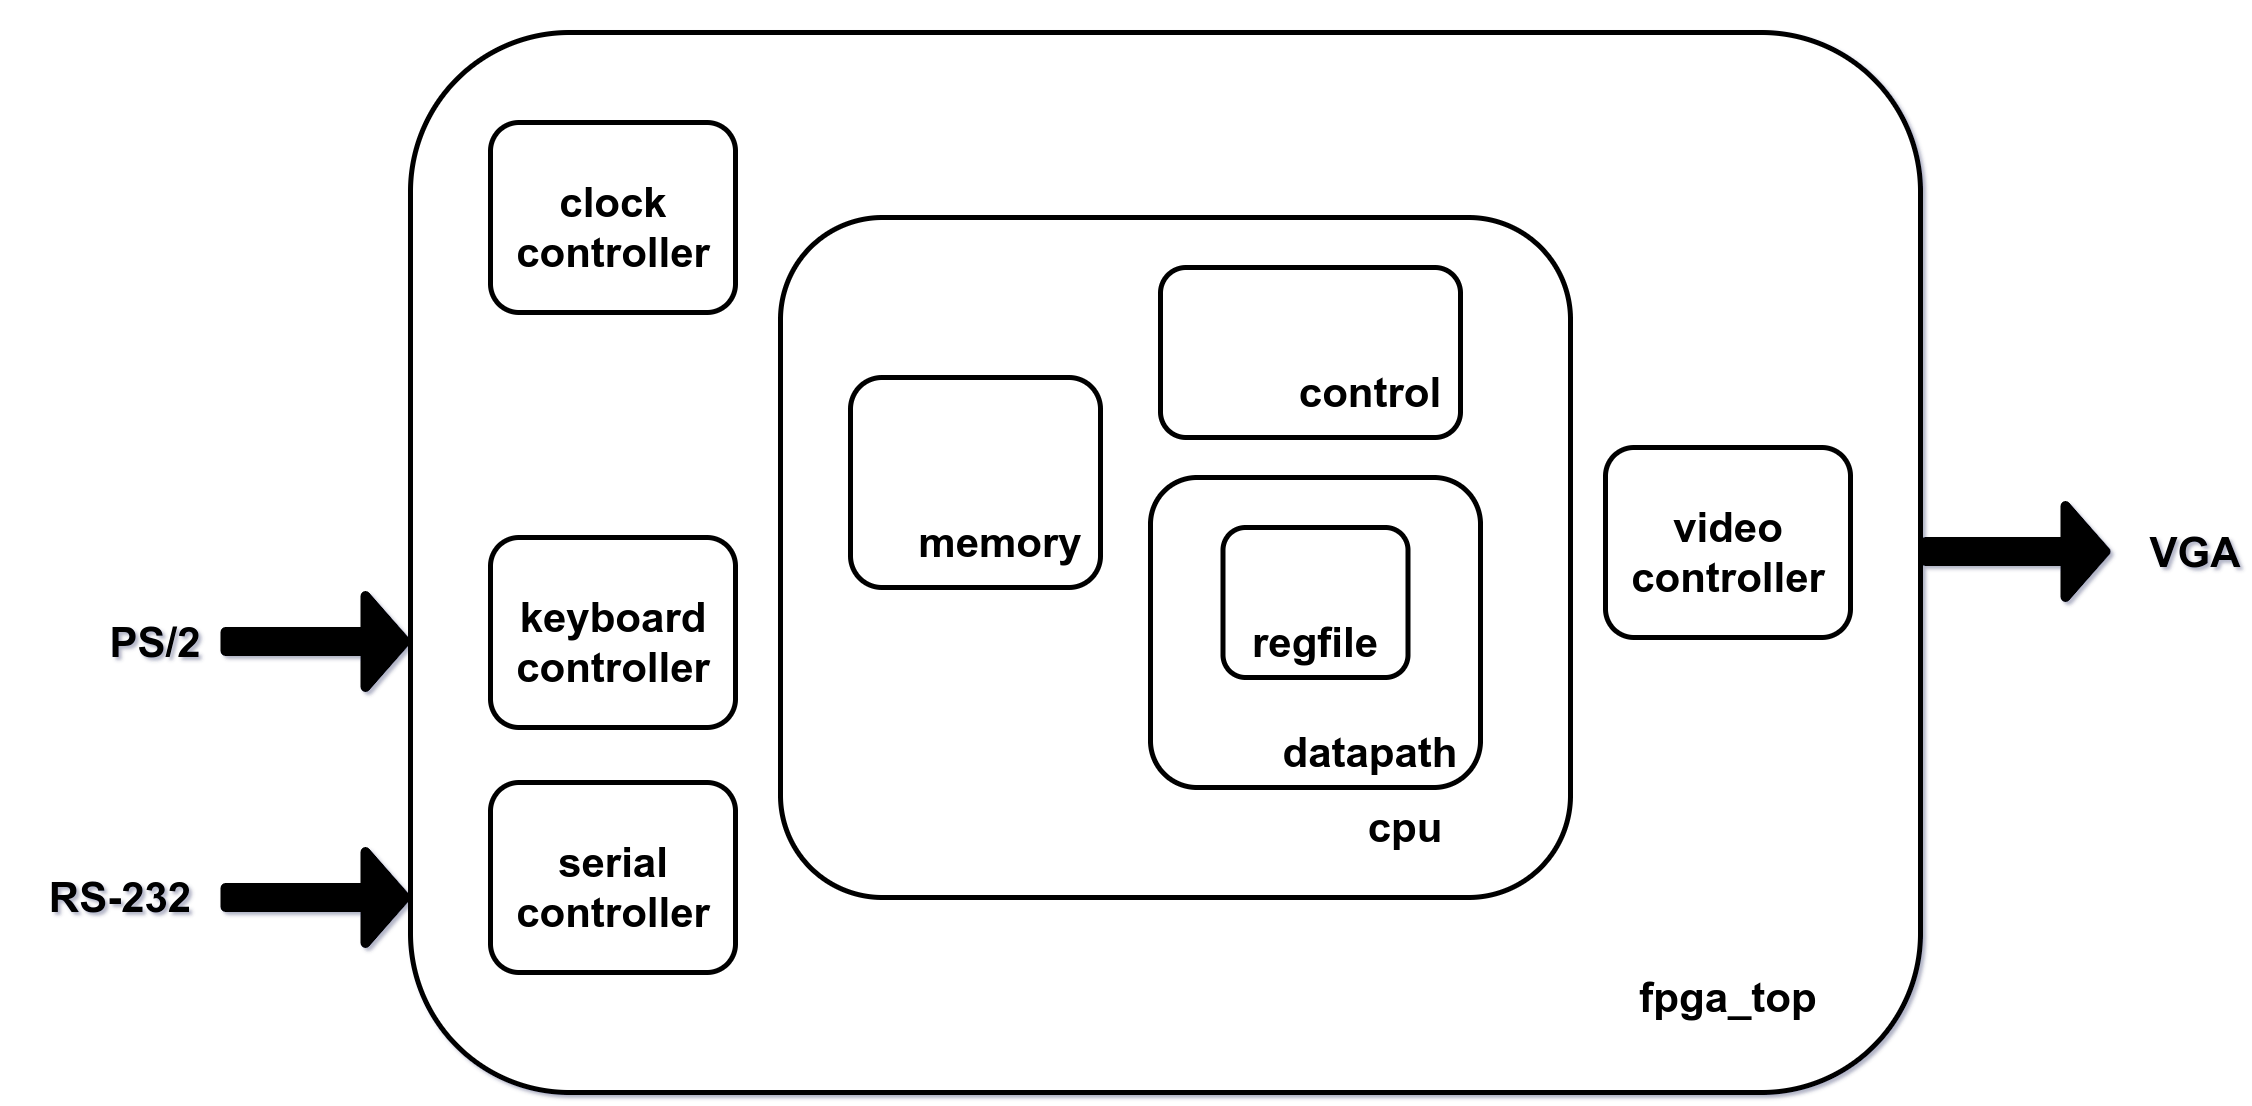
\includegraphics[width=0.9\linewidth]{../images/fpga/fpga_simplified_block_diagram.png}
        \caption{Diagrama de blocos simplificado do sistema}\label{fig:diagram_fpga_blocks}
    \end{figure}

    {
        O arquivo \texttt{core/config.v} possui todas as opções de configuração,
        definição de parâmetros e endereçamento de memória dos módulos, facilitando
        escolher as extensões, microarquitetura e periféricos sintetizados. Outras
        pastas e arquivos relevantes serão discutidos nas próximas seções.
    }


\section{Implementação dos \textit{soft-cores}}
    { Todos os \textit{soft-cores} implementados possuem execução em ordem, sem
        \textit{branch prediction}, sem \textit{caching} de memória e sem
        \textit{Return Address Stack}. O processador é escalar e possui um
        único \textit{hart}. Como a implementação atual só utiliza blocos de
        memória presentes no chip da FPGA, sem utilizar as memórias
        \textit{SRAM} e \textit{DRAM} externas presentes na placa de
        desenvolvimento, e também não faz uso de memória secundária, as operações
        de \textit{load} e \textit{store} transferem dados diretamente entre os
        registradores e os blocos de memória \textit{M10K}.
    }

    \subsection{Microarquitetura Uniciclo}

        { Os processsadores uniciclo com extensões I e IM são implementados
            conforme o diagrama da Figura~\ref{fig:diagram_rv32i_uni}. O módulo
            de controle é implementado somente com lógica combinacional, e a
            frequência máxima de operação é limitada pela instrução mais lenta
            do processador.
        }

        \begin{figure}[H]
        \centering
            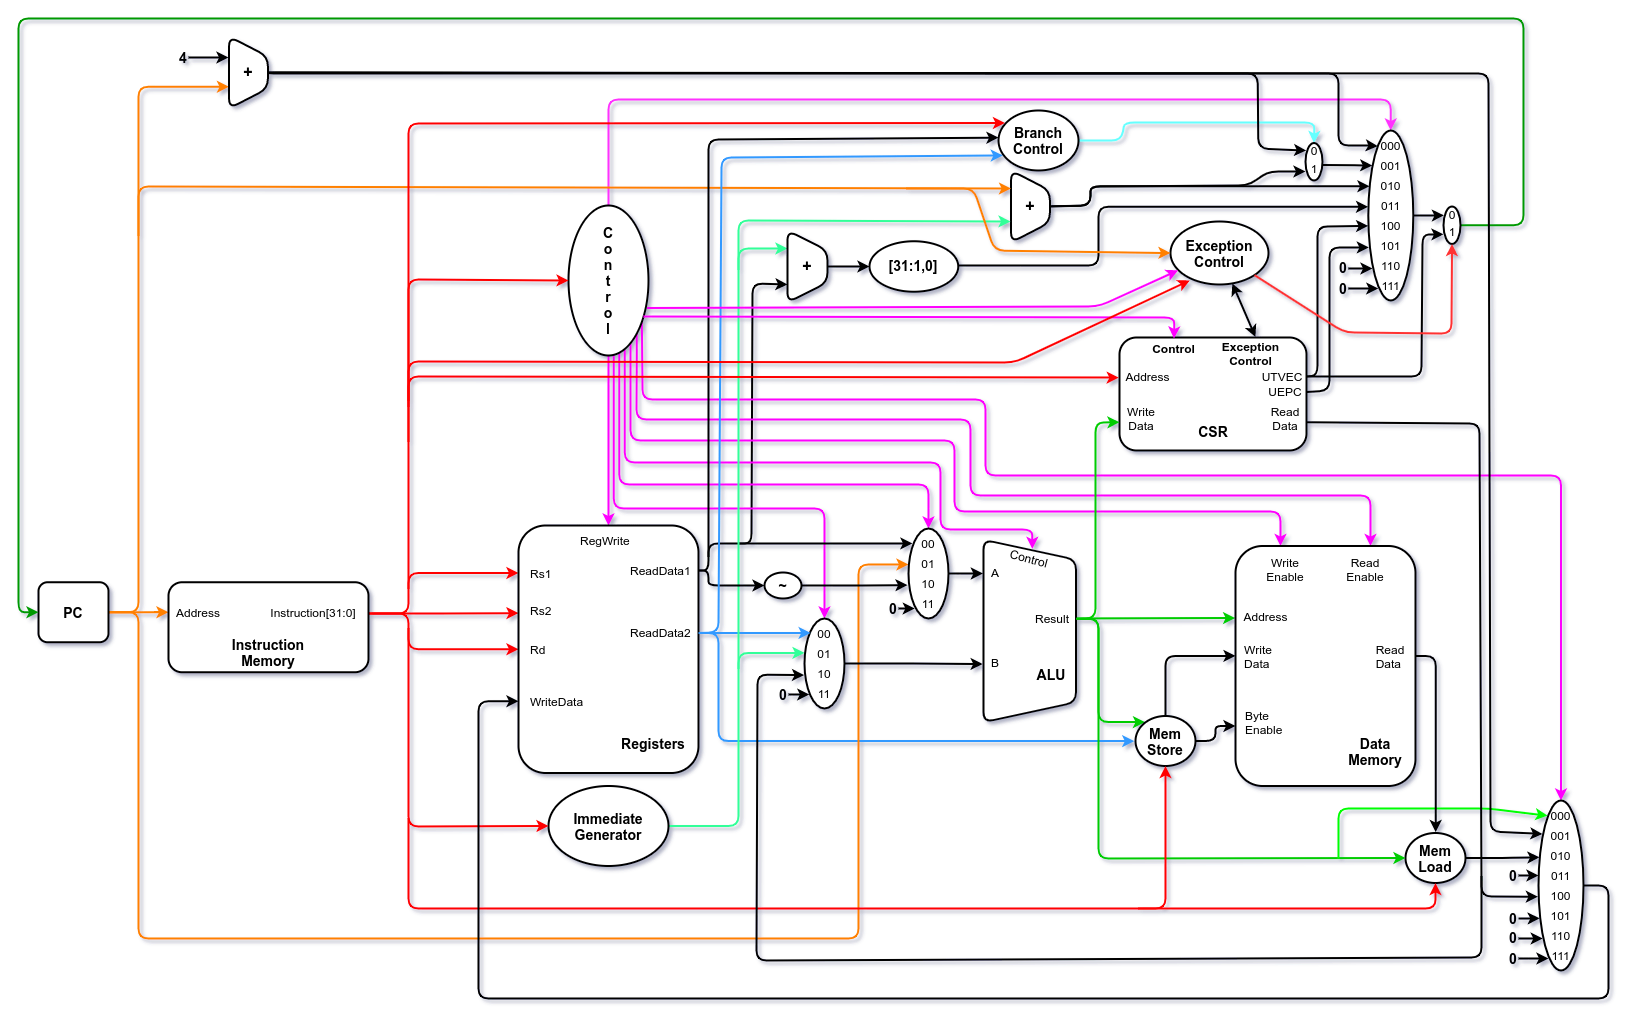
\includegraphics[width=.9\linewidth]{../images/uarch_diagrams/singlecycle-RV32I-RV32IM.png}
            \caption{Diagrama da implementação das \textit{ISAs} RV32I e RV32IM na
            microarquitetura uniciclo}\label{fig:diagram_rv32i_uni}
        \end{figure}

        { A instrução recuperada da memória de instruções \texttt{core/memory/CodeMemory\_Interface}
            no endereço apontado pelo registrador \texttt{PC} é lida pela unidade de controle
            \texttt{core/risc\_v/Control\_UNI .v}, que gera todos os sinais de
            controle enviados ao \textit{datapath} \texttt{core/risc\_v/Datapath\_Uni.v}.
        }

        {
            O banco de registradores \texttt{core/risc\_v/Registers.v} também
            recebe alguns \textit{bits} da instrução (para endereçamento dos
            registradores) e os dados para possivelmente serem escritos no registrador
            \texttt{rd} provenientes do multiplexador de \textit{write-back}.
        }

        { A unidade de lógica e aritmética \texttt{core/risc\_v/ALU.v} possui um
            multiplexador em cada uma de suas entradas para selecionar os operandos.
        }

        {
            Já a memória de dados \texttt{core/memory/DataMemory\_Interface.v}
            recebe o endereço de escrita/leitura vindo da saída da ULA, e suas
            operações de \textit{load/store} são comandadas pelos controladores
            \texttt{core/memory/MemLoad.v} e \texttt{core/memory/MemStore.v}.
        }

        { O banco de registradores de contorle e estado \texttt{core/risc\_v/CSRegisters.v}
            também é endereçado pela instrução, e o dado que possivelmente será
            gravado origina da ULA.
        }

        { Há ainda as unidades de controle de exceção \texttt{core/risc\_v/ExceptionControl.v},
            responsável por redirecionar o contador de programa \texttt{PC} para
            o endereço do \textit{kernel} quando ocorre uma exceção, como uma
            instrução inválida ou um endereço desalinhado. A unidade de controle
            de \textit{branches} \texttt{core/risc\_v/BranchControl.v} é responsável
            por rotear o endereço da próxima instrução caso ocorra um \textit{branch}
            ou \textit{jump}.
        }

        { A única diferença entre a implementação da \textit{ISA RV32I} e da
            \textit{RV32IM} é a adição de novas operações na unidade de lógica e
            aritmética.
        }

        { O processador uniciclo com extensão IMF é implementado conforme o
            diagrama da Figura~\ref{fig:diagram_rv32imf_uni}. A unidade lógica e
            aritmética de ponto flutuante utiliza uma frequência de \textit{clock}
            maior que a do resto do processador, e é o único módulo da implementação
            uniciclo que utiliza mais de um ciclo de relógio para realizar sua
            operação. A frequência máxima de operação do \textit{clock} principal
            do processador continua limitada pela operação mais lenta.
        }

        { Exceto o roteamento extra do banco de registadores \texttt{core/risc\_v/FRegisters.v}
            de ponto flutuante e da ULA de ponto flutuante de precisão simples
            \texttt{core/risc\_v/FPULA/FPALU.v}, o restante do circuito segue as mesmas conexões.
        }

        \begin{figure}[H]
        \centering
            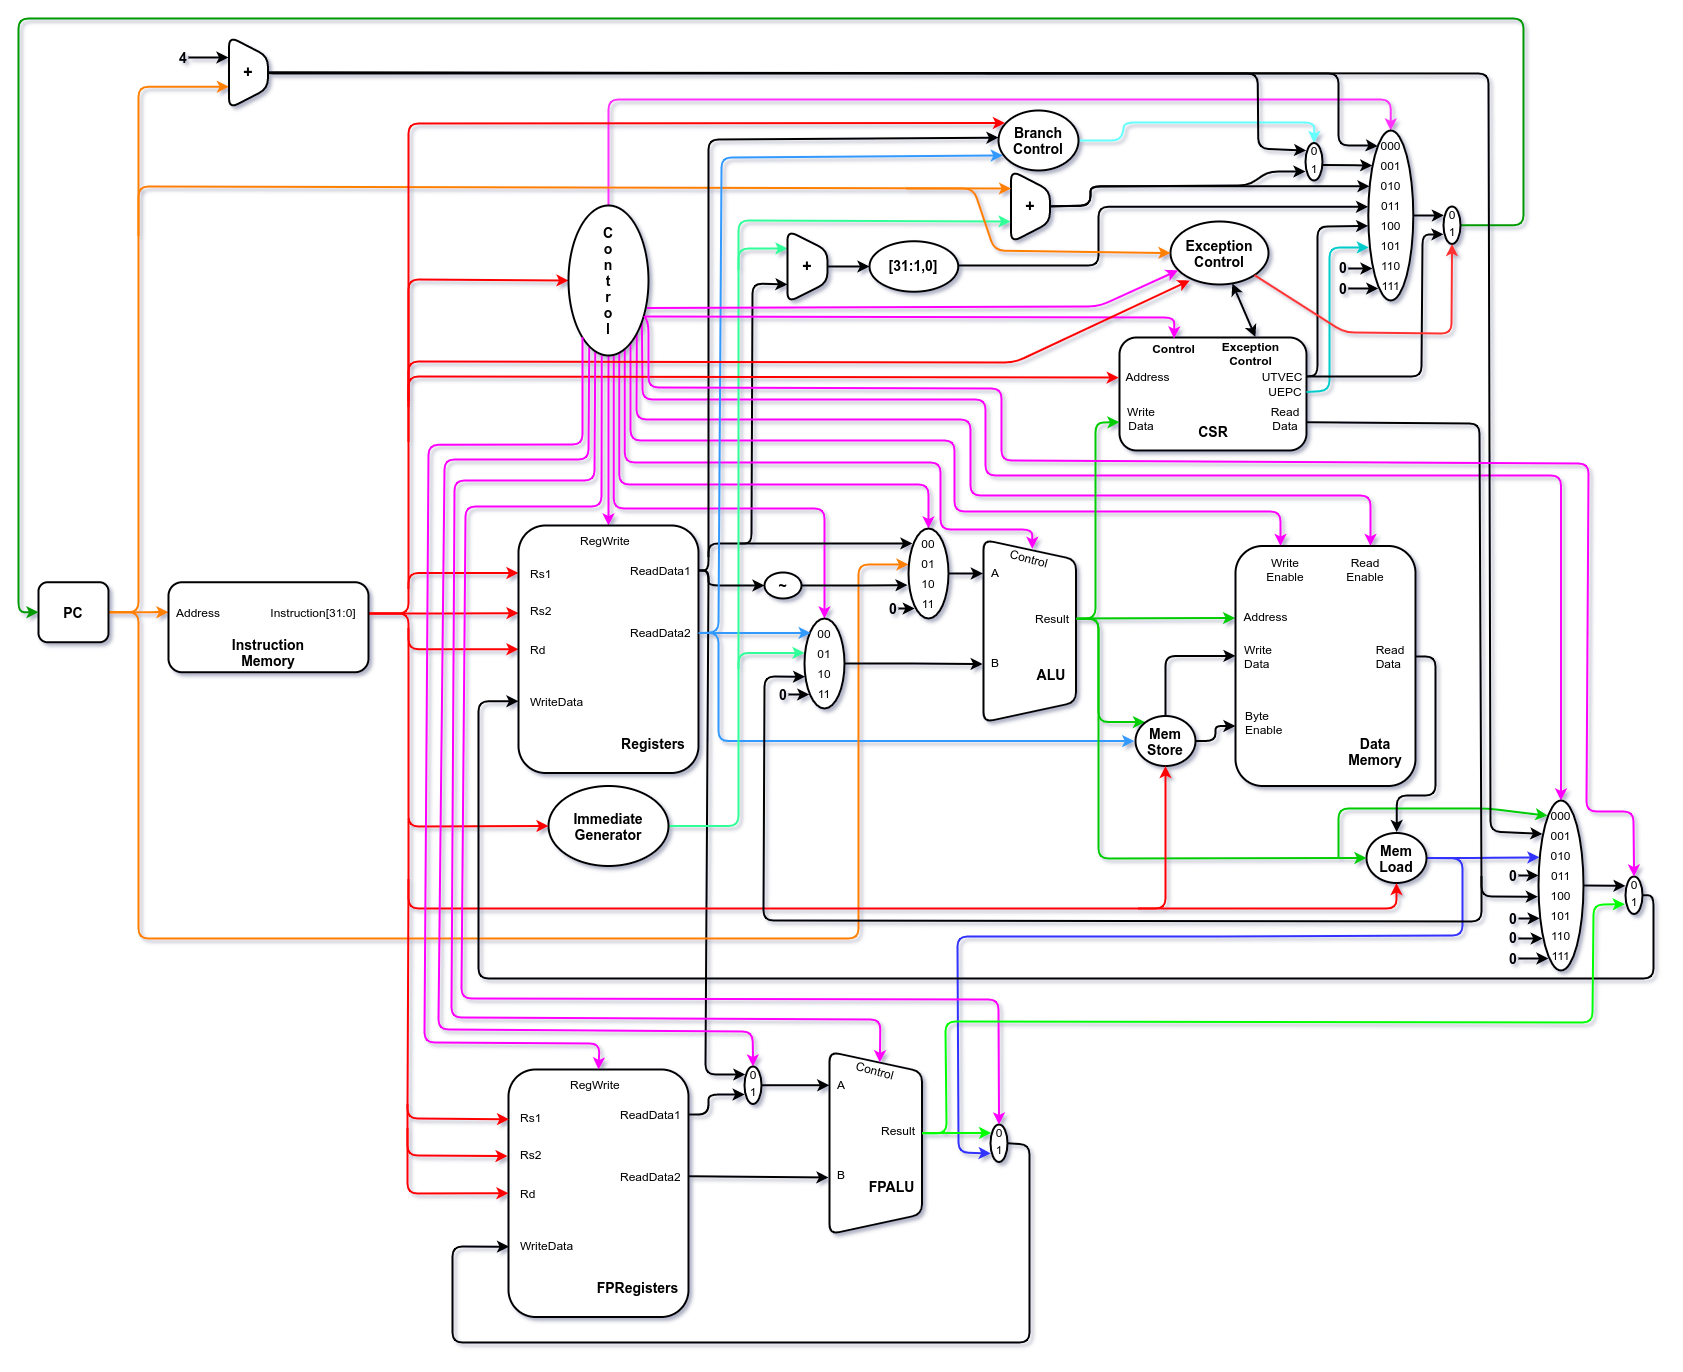
\includegraphics[width=.9\linewidth]{../images/uarch_diagrams/singlecycle-RV32IMF.png}
            \caption{Diagrama da implementação da \textit{ISA} RV32IMF na
            microarquitetura uniciclo}\label{fig:diagram_rv32imf_uni}
        \end{figure}

    \subsection{Microarquitetura Multiciclo}
        { Os processadores multiciclo com extensões I e IM são implementados
            conforme o diagrama da Figura~\ref{fig:diagram_rv32i_multi}. A
            unidade de controle é implementada utilizando microcódigo para
            executar as instruções. Com isso, a frequência de operação do
            processador depende da operação mais lenta do microcódigo, e não da
            execução da instrução completa.
        }

        { Enquanto as outras implementações usam arquitetura de memória \textit{Harvard},
            onde a memória de dados e a de instruções são separadas~\cite{harvard_arch},
            o multiciclo utiliza arquitetura \textit{von Neumann}, onde não há
            separação entre a memória de dados e a de texto~\cite{von_neumann_arch}.
        }

        {
            O módulo de memória \texttt{core/memory/Memory\_Interface.v} tem seu
            acesso controlado pelos blocos \texttt{core/memory/MemLoad.v} e
            \texttt{core/memory/MemStore}, além dos sinais vindos da unidade de
            controle \texttt{core/risc\_v/Control\_Multi.v}.
        }

        { A outra grande diferença em relação à implementação do uniciclo é que a
            saída do bloco de memória, dos dados do banco de registradores, da saída
            da ULA e do banco de registradores de controle e estado. Há também
            o registrador \texttt{PCBack} que salva o contador de programa atual.
        }

        { Além de alguns sinais em posições diferentes nos multiplexadores de seleção
            das entradas da ULA, de novo contador de programa e de \textit{write back},
            a atualização do contador de programa depende de uma comparação lógica.
        }

        { Com o controlador \texttt{core/risc\_v/Control\_Multi.v} implementado
            por microcódigo, as instruções possuem variação na quantidade de
            ciclos para serem completadas.
        }

        \begin{figure}[H]
        \centering
            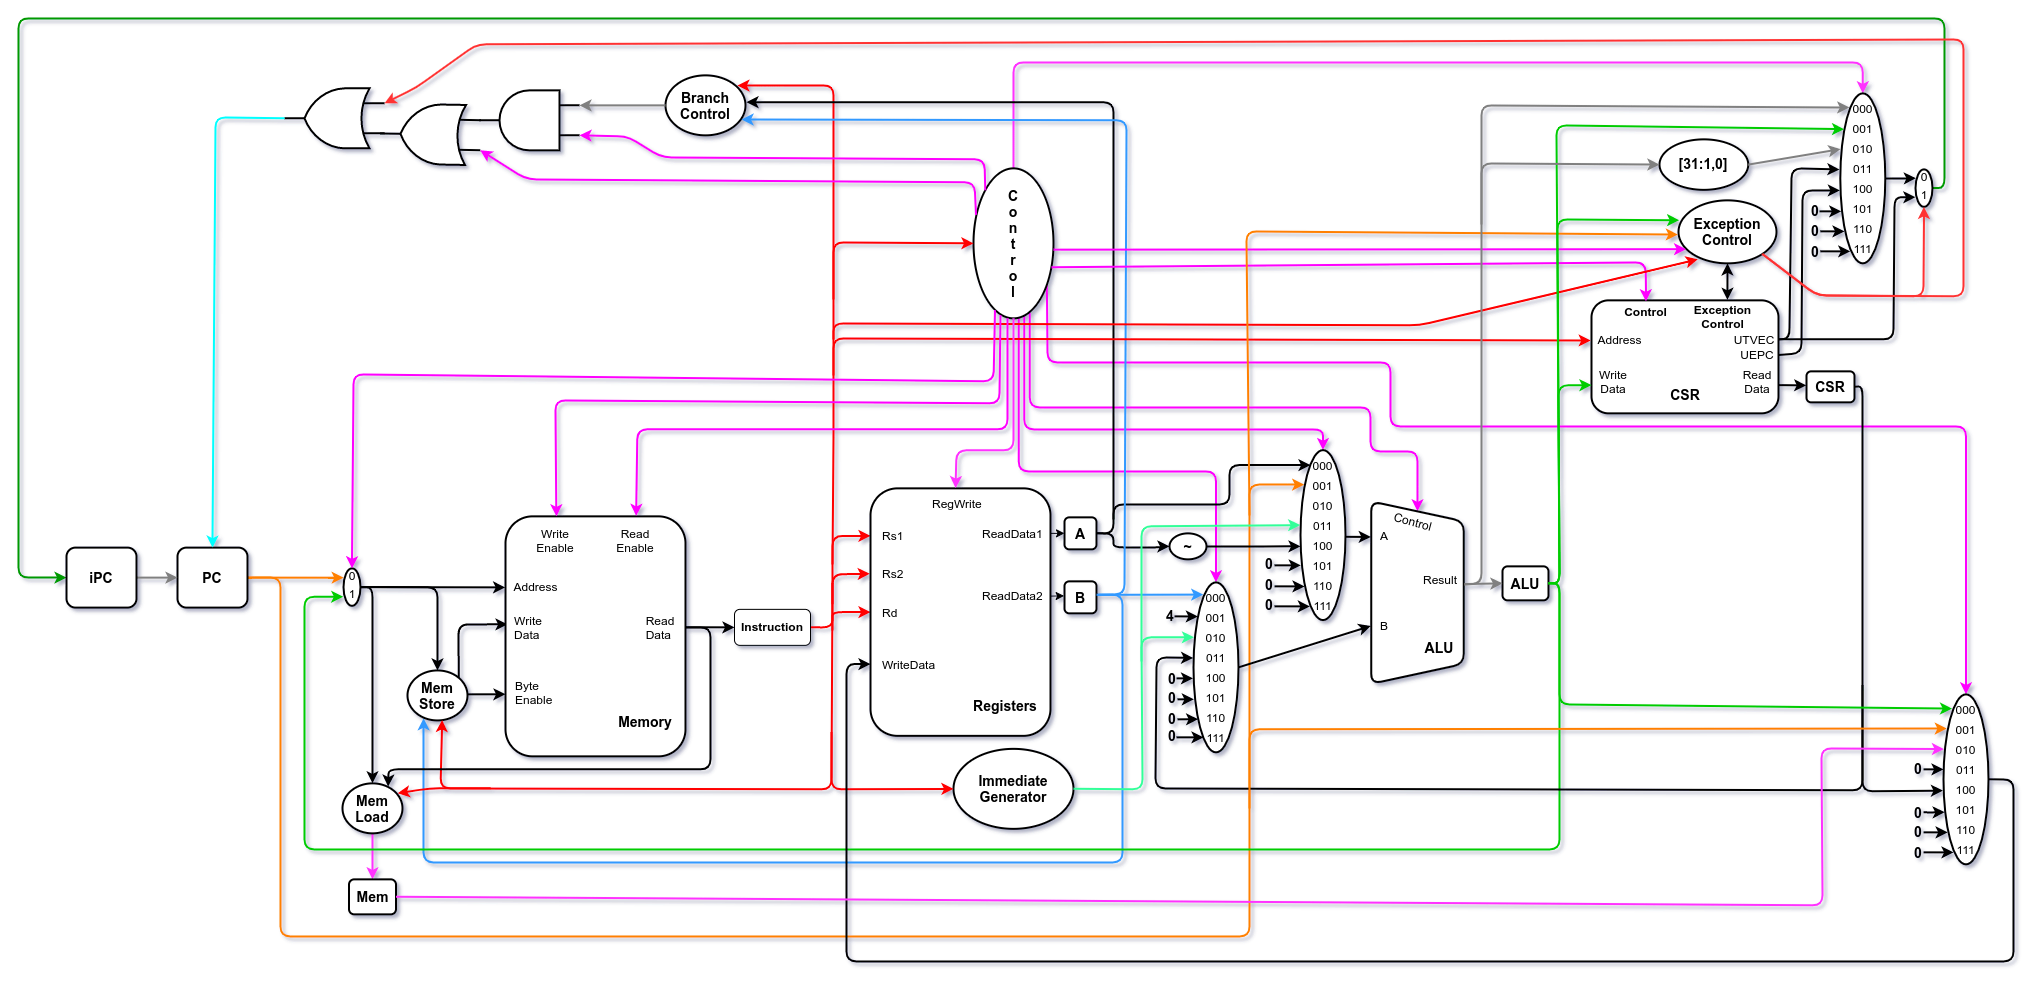
\includegraphics[width=.9\linewidth]{../images/uarch_diagrams/multicycle-RV32I-RV32IM.png}
            \caption{Diagrama da implementação das \textit{ISAs} RV32I e RV32IM na
            microarquitetura multiciclo}\label{fig:diagram_rv32i_multi}
        \end{figure}

        { O processador multicilo com extensões IMF é implementado conforme o
            diagrama da Figura~\ref{fig:diagram_rv32imf_multi}. A unidade lógica
            e aritmética de ponto flutuante utiliza uma frequência de \textit{clock}
            mais alta que a do resto do processador, e possui um sinal de
            \textit{ready} que causa o \textit{stall} do clock principal do
            processador enquanto a operação de ponto flutuante não completa.
            Assim, a frequência do \textit{clock} do processador é variável, já
            que em operações de ponto flutuante o ciclo do relógio é mais longo
            que em outras operações.
        }

        { A diferença entre o conjunto de instruções com e sem a extensão \textbf{F}
            é a presença do banco de registradores e a unidade de ponto flutuante,
            que também possuem suas saídas registradas.
        }

        { A presença dos registradores nas saídas dos módulos de onde dados são
            lidos servem para criar um atraso de um ciclo de \textit{clock} nesses
            valores. Como a unidade de controle utiliza microcódigo, o dado lido
            no ciclo atual só será utilizado no próximo ciclo.
        }

        \begin{figure}[H]
        \centering
            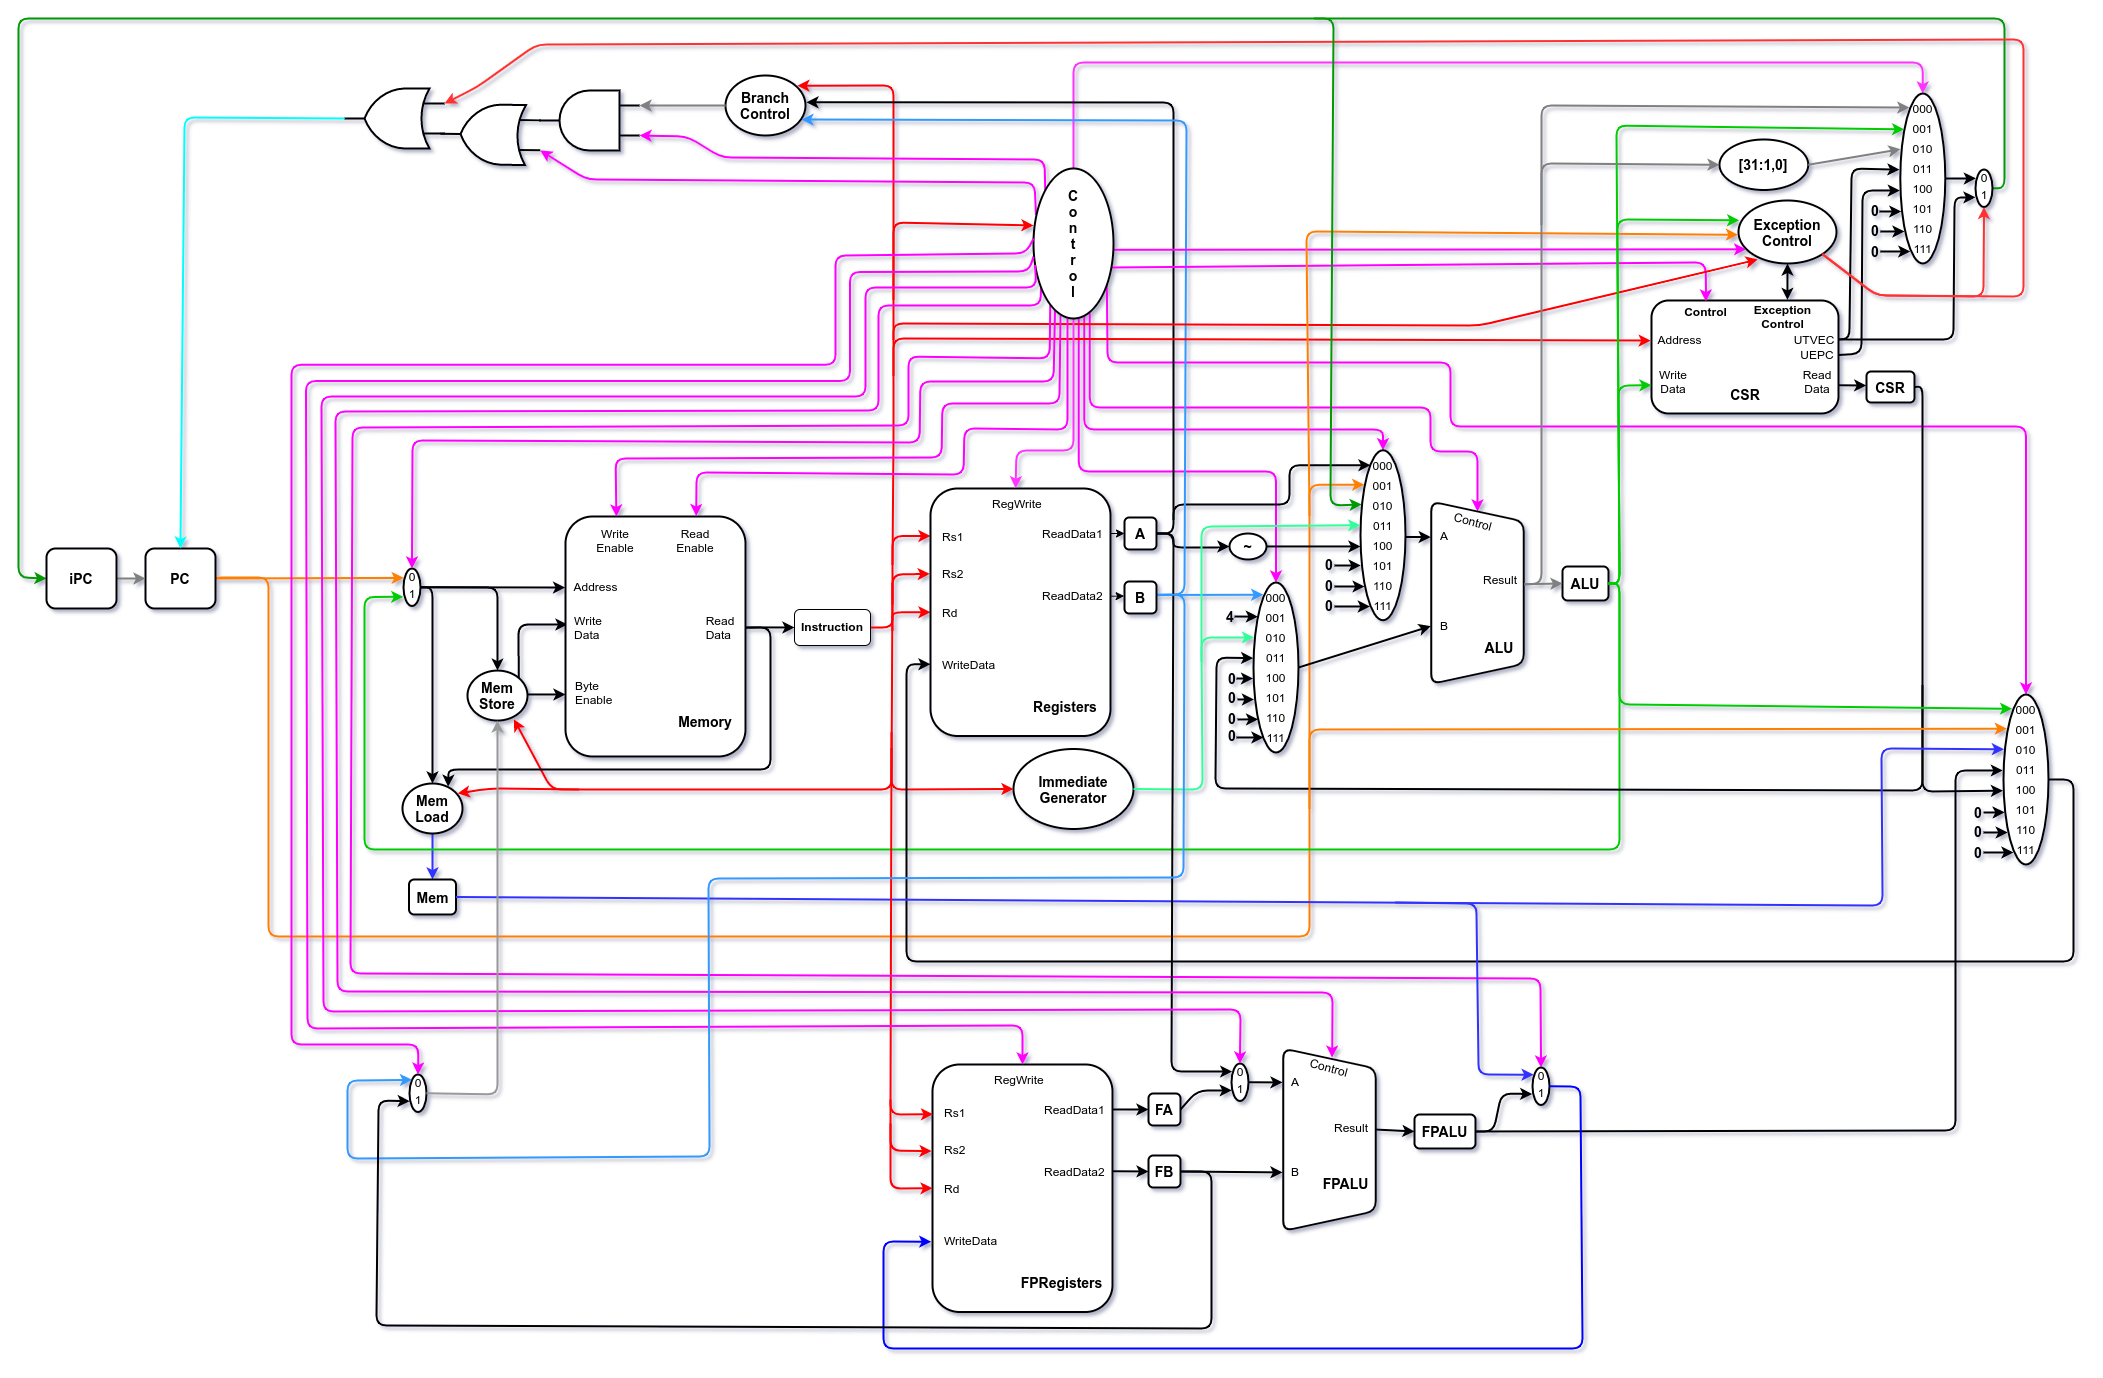
\includegraphics[width=.9\linewidth]{../images/uarch_diagrams/multicycle-RV32IMF.png}
            \caption{Diagrama da implementação da \textit{ISA} RV32IMF na
            microarquitetura multiciclo}\label{fig:diagram_rv32imf_multi}
        \end{figure}


    \subsection{Microarquitetura \textit{Pipeline} de 5 Estágios}
        { Os processadores \textit{pipeline} com extensões I e IM são
            implementados conforme o diagrama da Figura~\ref{fig:diagram_rv32i_pipe}.
            Seus cinco estágios são:
            \begin{enumerate}
                \item \textit{IF - Instruction Fetch}
                \item \textit{ID - Instruction Decode}
                \item \textit{EX - Execution}
                \item \textit{MEM - Memory Stage}
                \item \textit{WB - Write Back}
            \end{enumerate}
        }

        { No primeiro estágio (\textit{IF}) estão presentes o contador de programa,
            a memória de instruções e um somador que incrementa o \texttt{PC} em 4
            bytes, que será o endereço da instrução seguinte caso não ocorra um
            \textit{branch, jump}, exceção ou \textit{syscall}.
        }

        { Entre os estágios de \textit{Instruction Fetch} e \textit{Instruction
            Decode}, existe um grupo de registradores (\textit{IFID}) responsável
            por passar os valores do primeiro estágio para o seguinte.
        }

        \begin{figure}[H]
        \centering
            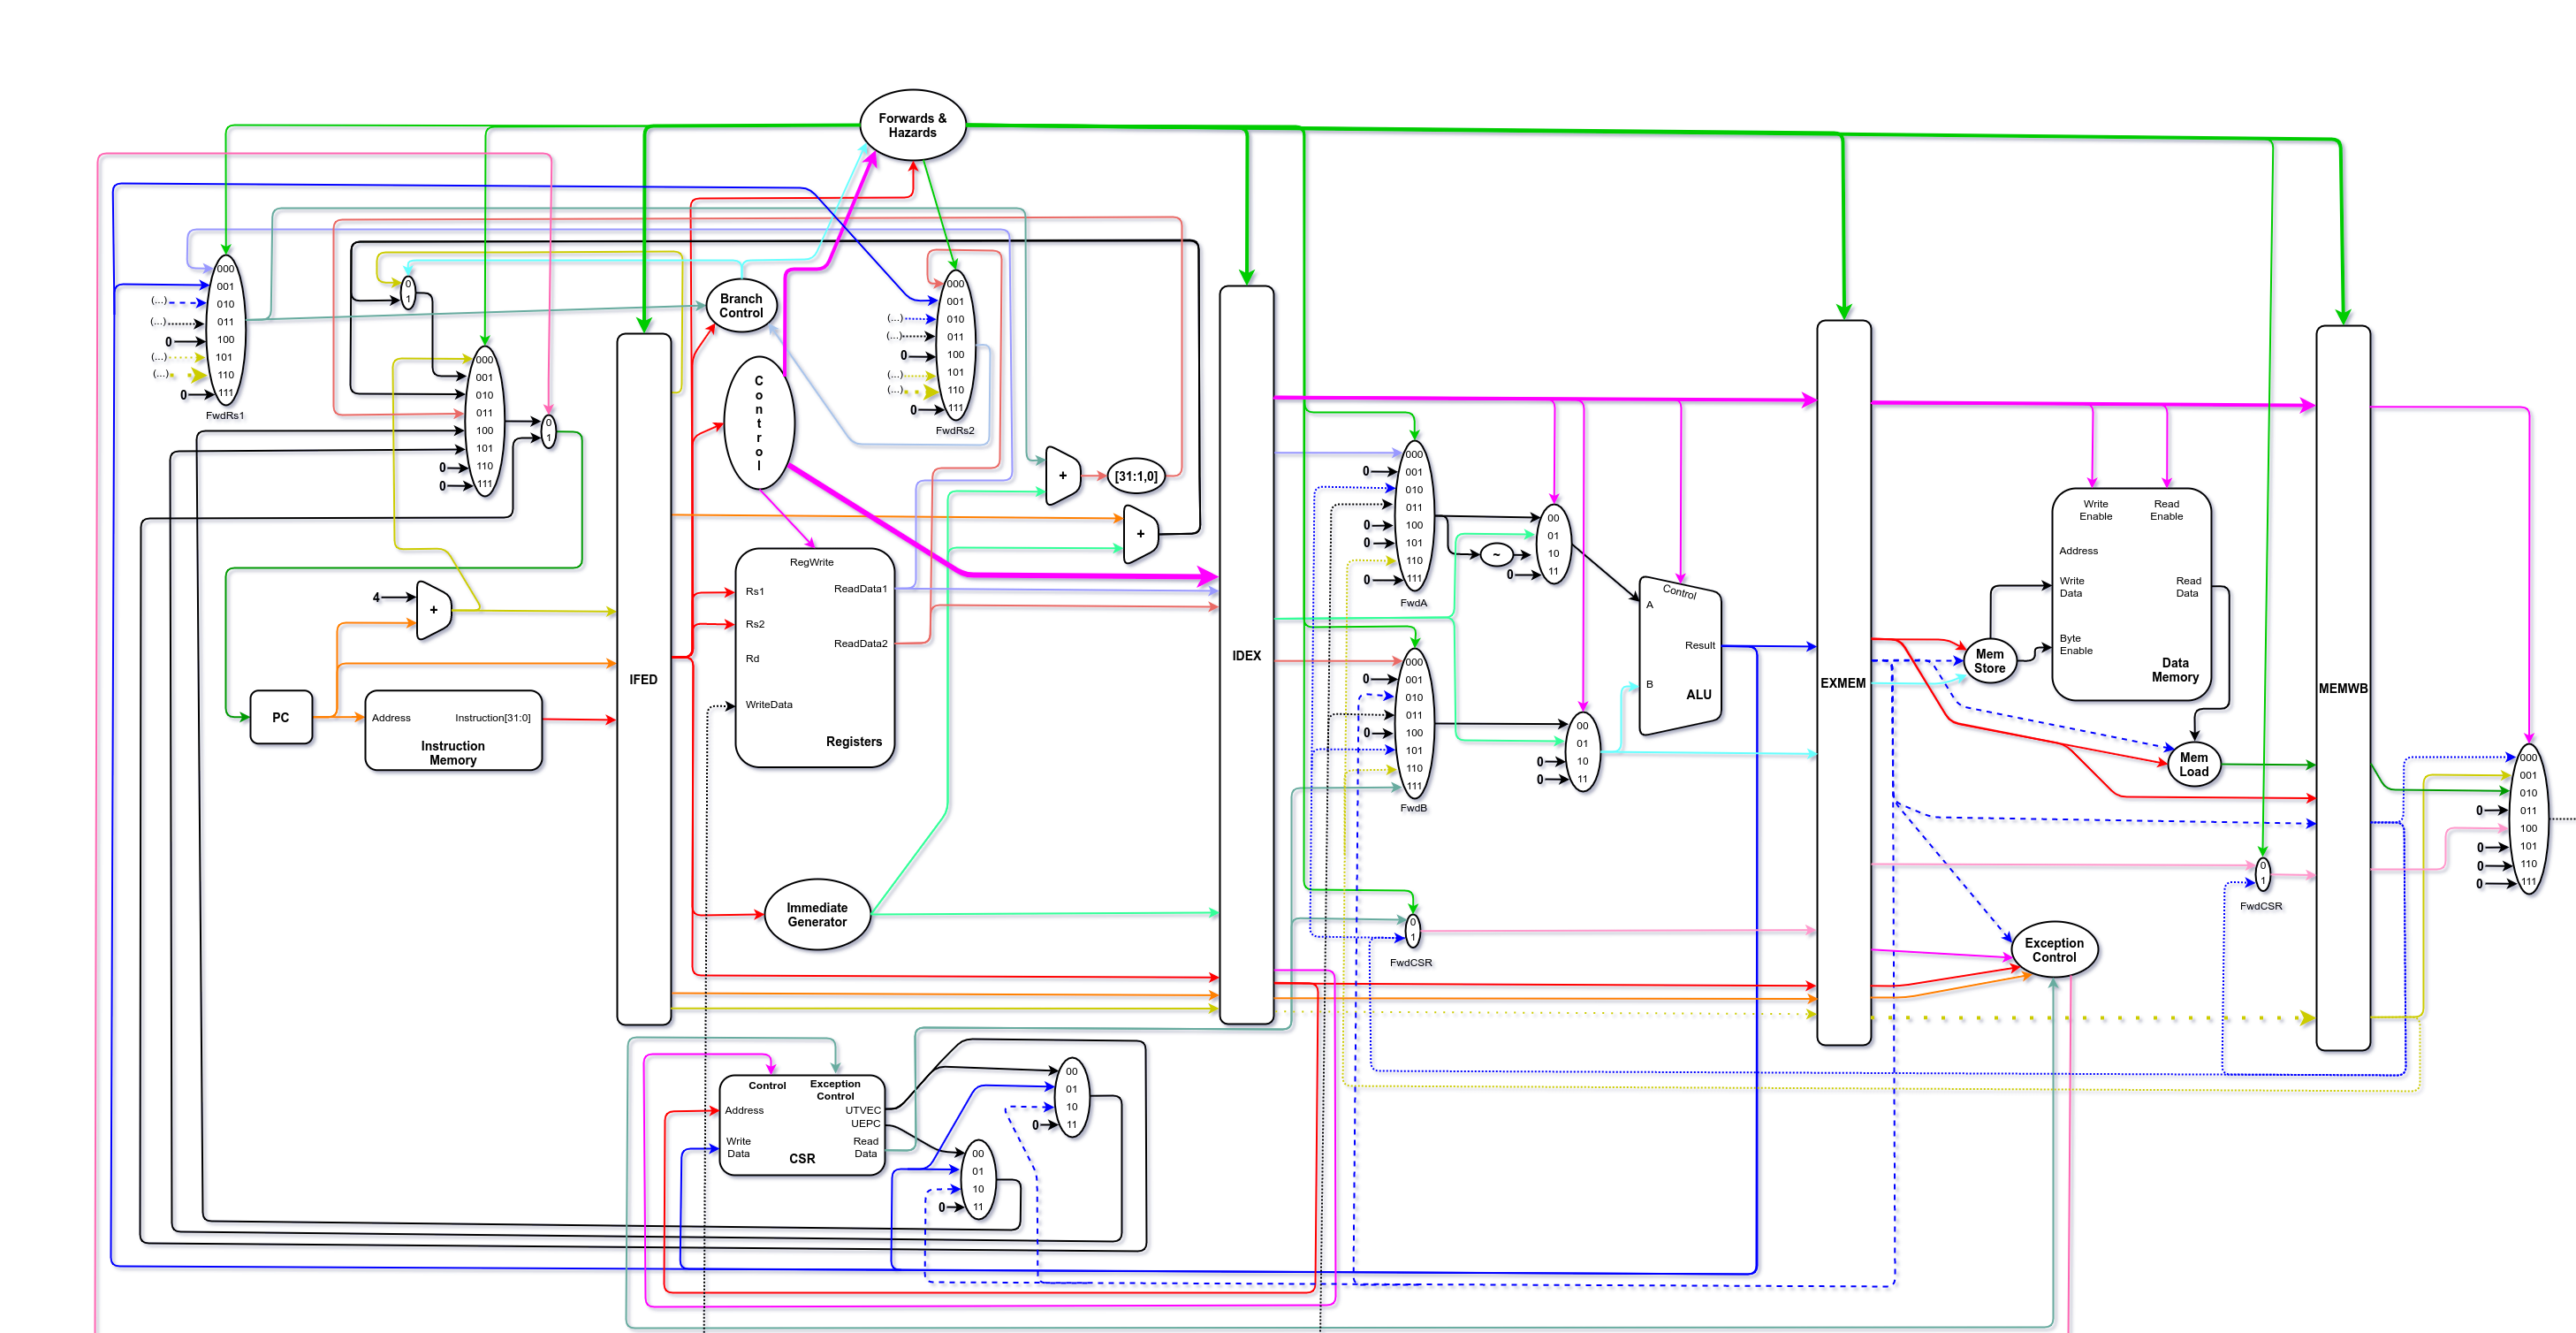
\includegraphics[width=.9\linewidth]{../images/uarch_diagrams/pipeline-RV32I-RV32IM.png}
            \caption{Diagrama das \textit{ISAs} RV32I e RV32IM na microarquitetura
                \textit{pipeline} de 5 estágios}\label{fig:diagram_rv32i_pipe}
        \end{figure}

        { No segundo estágio (\textit{ID}) ocorre a decodificação da instrução.
            Também é o estágio onde ficam localizados o banco de registradores,
            os registradores de controle e estado, a unidade de geração de imediatos,
            a de controle de \textit{branches} e \textit{jumps}, além da unidade
            de \textit{forwards} e \textit{hazards} \texttt{core/risc\_v/FwdHazardUnitM.v}.
        }

        { A unidade de \textit{forwards} e \textit{hazards} é essencial para o
            bom funcionamento e desempenho do \textit{pipeline}. Brevemente discutida
            na Seção~\ref{cap2_fwd_hzd}, \textit{hazards} ocorrem quando uma instrução
            a partir do segundo estágio tem como entrada um dado que ainda não foi
            calculado. É o caso do código a seguir:
        }
        \begin{lstlisting}
    0x00400000:     la  t1, 8
    0x00400004:     lw  t0, 0(t1)
        \end{lstlisting}

        { Quando a instrução \texttt{lw  t0, 0(t1)} está calculando o endereço
            do \textit{load} \texttt{(t1 + 0)}, o valor de \texttt{t1} ainda
            não foi salvo no banco de registradores, e por isso não pode ser
            lido. Os \textit{forwards} identificam situações como essa e injetam
            o sinal calculado, ``furando'' a ordem do \textit{pipeline}.
            Já em casos onde não é possível recuperar o valor necessário de uma
            etapa seguinte, ocorreu um \textit{hazard} e um \texttt{nop} precisa
            ser inserido no \textit{pipeline}, passando um ou mais ciclos sem
            processar novas instruções.
        }

        { Entre os estágios de \textit{Instruction Decode} e \textit{Execution},
            existe um grupo de registradores (\textit{IDEX}) responsável por passar
            os valores do segundo estágio para o terceiro. No terceiro estágio
            (\textit{EX}) ocorrem as operações lógicas e aritméticas.
            Os seletores das entradas da ULA recebem diversos sinais para
            possibilitar os \textit{forwards} de dados.
        }

        { A frequência máxima do \textit{clock} do processador é limitada pela
            operação mais lenta da unidade lógica e aritmética.
        }

        { Entre os estágios de \textit{Execution} e \textit{Memory Stage},
            existe um grupo de registradores (\textit{EXMEM}) responsável por passar
            os valores do terceiro estágio para o quarto. No quarto estágio
            (\textit{MEM}) é feito o acesso à memória. A unidade
            de controle de exceções também se encontra nesse estágio. A leitura
            da memória ocorre no ciclo positivo do relógio, enquanto a escrita
            é feita na borda de descida.
        }

        { Entre os estágios de \textit{Memory Stage} e \textit{Write Back},
            existe um grupo de registradores (\textit{MEMWB}) responsável por passar
            os valores do quarto estágio para o quinto e último estágio. No quinto
            estágio (\textit{WB}) é feita a escrita no banco de registradores.
            O sinal com o dado a ser escrito, bem como o endereço do registrador,
            é injetado no estágio \textit{ID}, finalizando o ciclo de vida da
            instrução dentro do \textit{pipeline}.
        }

        \begin{figure}[H]
        \centering
            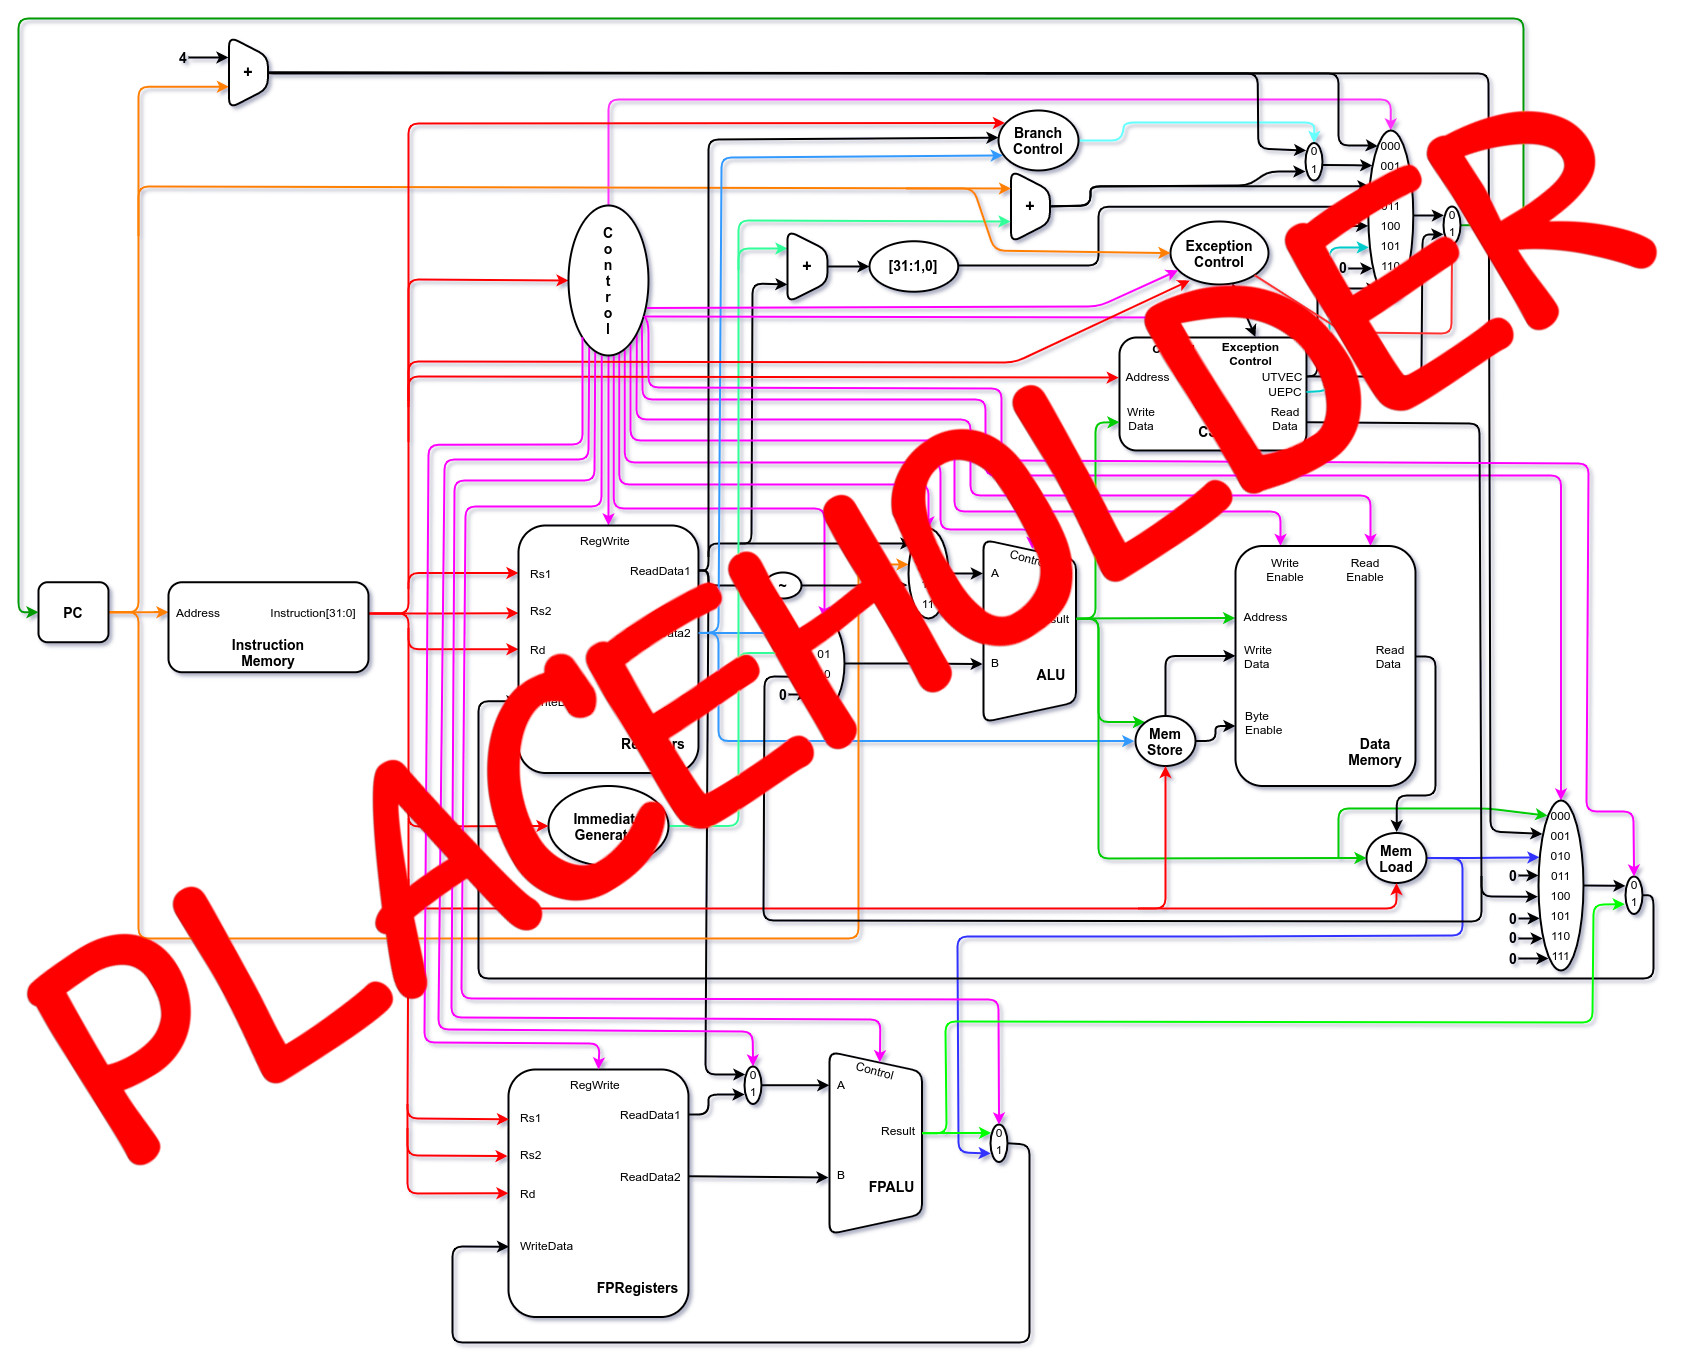
\includegraphics[width=.9\linewidth]{../images/uarch_diagrams/pipeline-RV32IMF.png}
            \caption{Diagrama da \textit{ISA} RV32IMF na microarquitetura
                \textit{pipeline} de 5 estágios}\label{fig:diagram_rv32imf_pipe}
        \end{figure}

        { O processador \textit{pipeline} com extensões \textbf{IMF} é implementado
            conforme o diagrama da Figura~\ref{fig:diagram_rv32imf_pipe}. Sua
            diferença entre o sistema descrito anteriormente é a presença do
            banco de registradores de ponto flutuante no estágio \textit{ID} e
            da \textit{FPALU} no estágio \textit{EX}.
        }

\section{Chamadas de sistema}
    { A pasta \texttt{system} contém a implementação das chamadas de sistema do
        processador. O código \textit{assembly} deve incluir o arquivo
        \texttt{system/MACROS.s} no início do programa e o arquivo
        \texttt{system/SYSTEM.s} ao final do programa.
    }
    \begin{lstlisting}
# Inicio do programa
.include "MACROS.s"

# Dados do programa
.data
    ...

# Instrucoes do programa
.text
    ...

# Chamadas de sistema
.include "SYSTEM.s"
    \end{lstlisting}

    { O arquivo \texttt{MACROS.s} insere macros que testam se o programa
        está sendo executado no \texttt{Rars}, na \texttt{FPGA} ou no
        \texttt{ModelSim} para decidir o uso de determinadas \textit{syscalls},
        e também fornece a implementação por \textit{software} de algumas
        instruções caso a extensão necessária não esteja implementada no processador,
        como instruções de multiplicação. Os endereços de memória dos periféricos
        acessados por \textit{MMIO} também estão presentes como definições
        \texttt{.eqv} para facilitar a implementação dos programas.
    }

    { Já o arquivo \texttt{SYSTEM.s} implementa o \textit{kernel} do sistema,
        tratando exceções e executando as \textit{syscalls}. As chamadas de
        sistema implementadas são apresentadas na Tabela~\ref{table:syscalls}.
    }

    { Como o processador implementado não possui memória reservada para o
        \textit{kernel}, sua posição inicial de memória começa imediatamente
        após a última instrução do programa implementado, e por isso deve ser
        incluído no final do arquivo. O arquivo de macros deve ser adicionado
        no início do programa, pois ele é responsável por gravar o endereço inicial
        do nível privilegiado no \textit{CSR UTVEC} e ativar as interrupções.
    }

    \begin{longtable}{|l|c|p{3cm}|l |}
        \caption{Tabela de \textit{syscalls} implementadas.}\label{table:syscalls}\\
        \hline
        \textit{syscall}                    & \texttt{a7}             & Argumentos                & Operação\\*
        \hline
        \endfirsthead
        \hline
        \textit{syscall}                    & \texttt{a7}             & Argumentos                & Operação\\*
        \hline
        \endhead
        \multirow{5}{*}{Print Integer}      & \multirow{5}{*}{\parbox{0.6cm}{\centering 1 ou 101}}
              & \texttt{a0 =} inteiro     & \multirow{5}{*}{\parbox{7cm}{Imprime no \textit{frame} \texttt{a4} o número inteiro \texttt{a0} (complemento de 2) na
                                                posição \texttt{(a1,a2)} com as cores \texttt{a3[7:0]} de \textit{foreground} e \texttt{a3[15:8]} de \textit{background}.}}\\*
            & & \texttt{a1 =} coluna      & \\*
            & & \texttt{a2 =} linha       & \\*
            & & \texttt{a3 =} cores       & \\*
            & & \texttt{a4 =} frame       & \\
        \hline
        \multirow{5}{*}{Print Float}        & \multirow{5}{*}{\parbox{0.6cm}{\centering 2 ou 102}}
              & \texttt{fa0 =} float      & \multirow{5}{*}{\parbox{7cm}{Imprime no \textit{frame} \texttt{a4} o número de ponto flutuante \texttt{fa0} na
                                                posição \texttt{(a1,a2)} com as cores \texttt{a3[7:0]} de \textit{foreground} e \texttt{a3[15:8]} de \textit{background}.}}\\*
            & & \texttt{a1 =} coluna      & \\*
            & & \texttt{a2 =} linha       & \\*
            & & \texttt{a3 =} cores       & \\*
            & & \texttt{a4 =} frame       & \\
        \hline
        \multirow{5}{*}{Print String}       & \multirow{5}{*}{\parbox{0.6cm}{\centering 4 ou 104}}
              & \texttt{a0 =} endereço da string  & \multirow{5}{*}{\parbox{7cm}{Imprime no \textit{frame} \texttt{a4} a \textit{string} iniciada no endereço \texttt{a0} e terminada
                                                        em \textit{NULL} na posição \texttt{(a1,a2)} com as cores \texttt{a3[7:0]} de \textit{foreground} e \texttt{a3[15:8]} de \textit{background}.}}\\*
            & & \texttt{a1 =} coluna      & \\*
            & & \texttt{a2 =} linha       & \\*
            & & \texttt{a3 =} cores       & \\*
            & & \texttt{a4 =} frame       & \\
        \hline
        \multirow{3}{*}{Read Int}           & \multirow{3}{*}{\parbox{0.6cm}{\centering 5 ou 105}}
            &                               & \multirow{3}{*}{\parbox{7cm}{Retorna em \texttt{a0} o valor do inteiro em complemento de 2 lido do teclado.}}\\*
            & & & \\*
            & & & \\
        \hline
        \multirow{3}{*}{Read Float}         & \multirow{3}{*}{\parbox{0.6cm}{\centering 6 ou 106}}
            &                               & \multirow{3}{*}{\parbox{7cm}{Retorna em \texttt{a0} o valor do \textit{float} com precisão simples lido do teclado.}}\\*
            & & & \\*
            & & & \\
        \hline
        \multirow{3}{*}{Read String}        & \multirow{3}{*}{\parbox{0.6cm}{\centering 8 ou 108}}
            & \texttt{a0 =} endereço do buffer    & \multirow{3}{*}{\parbox{7cm}{Escreve no \textit{buffer} iniciado em \texttt{a0} os caracteres lidos, terminando com um caracter \textit{NULL}.}}\\*
            & & \texttt{a1 =} número máximo de caracteres & \\*
            & & & \\
        \hline
        \multirow{3}{*}{Exit}               & \multirow{3}{*}{\parbox{0.6cm}{\centering 10 ou 110}}
            &                               & \multirow{3}{*}{\parbox{7cm}{Retorna ao sistema operacional. Na \textit{DE1-SoC}, trava o processador.}}\\*
            & & & \\*
            & & & \\
        \hline
        \multirow{5}{*}{Print Char}         & \multirow{5}{*}{\parbox{0.6cm}{\centering 11 ou 111}}
              & \texttt{a0 =} char ASCII  & \multirow{5}{*}{\parbox{7cm}{Imprime no \textit{frame} \texttt{a4} o caracter \texttt{a0} na
                                                posição \texttt{(a1,a2)} com as cores \texttt{a3[7:0]} de \textit{foreground} e \texttt{a3[15:8]} de \textit{background}.}}\\*
            & & \texttt{a1 =} coluna      & \\*
            & & \texttt{a2 =} linha       & \\*
            & & \texttt{a3 =} cores       & \\*
            & & \texttt{a4 =} frame       & \\
        \hline
        \multirow{3}{*}{Read Char}          & \multirow{3}{*}{\parbox{0.6cm}{\centering 12 ou 112}}
            &                               & \multirow{3}{*}{\parbox{7cm}{Retorna em \texttt{a0} o valor ASCII do caracter lido do teclado.}}\\*
            & & & \\*
            & & & \\
        \hline
        \multirow{3}{*}{Time}               & \multirow{3}{*}{\parbox{0.6cm}{\centering 30 ou 130}}
            &                               & \multirow{3}{*}{\parbox{7cm}{Retorna o tempo do sistema em \textit{ms}, com os 32 \textit{bits} menos significativos em \texttt{a0}
                                                e os 32 \textit{bits} mais significativos em \texttt{a1}.}}\\*
            & & & \\*
            & & & \\
        \hline
        \multirow{4}{*}{MIDI Out Assíncrono }   & \multirow{4}{*}{\parbox{0.6cm}{\centering 31 ou 131}}
              & \texttt{a0 =} pitch       & \multirow{4}{*}{\parbox{7cm}{Gera o som definido e retorna imediatamente.}}\\*
            & & \texttt{a1 =} duração (\textit{ms}) & \\*
            & & \texttt{a2 =} instrumento & \\*
            & & \texttt{a3 =} volume      & \\
        \hline
        \multirow{3}{*}{Sleep}              & \multirow{3}{*}{\parbox{0.6cm}{\centering 32 ou 132}}
            & \texttt{a0 =} duração (\textit{ms}) & \multirow{3}{*}{\parbox{7cm}{Coloca o processador em \textit{sleep} por \texttt{a1} \textit{ms}.}}\\*
            & & & \\*
            & & & \\
        \hline
        \multirow{4}{*}{MIDI Out Síncrono }     & \multirow{4}{*}{\parbox{0.6cm}{\centering 33 ou 133}}
              & \texttt{a0 =} pitch       & \multirow{4}{*}{\parbox{7cm}{Gera o som definido e retorna após o término da execução da nota.}}\\*
            & & \texttt{a1 =} duração (\textit{ms}) & \\*
            & & \texttt{a2 =} instrumento & \\*
            & & \texttt{a3 =} volume      & \\
        \hline
        \multirow{5}{*}{Print Integer}      & \multirow{5}{*}{\parbox{0.6cm}{\centering 34 ou 134}}
              & \texttt{a0 =} inteiro     & \multirow{5}{*}{\parbox{7cm}{Imprime no \textit{frame} \texttt{a4} o número inteiro \texttt{a0} em formato hexadecimal na
                                                posição \texttt{(a1,a2)} com as cores \texttt{a3[7:0]} de \textit{foreground} e \texttt{a3[15:8]} de \textit{background}.}}\\*
            & & \texttt{a1 =} coluna      & \\*
            & & \texttt{a2 =} linha       & \\*
            & & \texttt{a3 =} cores       & \\*
            & & \texttt{a4 =} frame       & \\
        \hline
        \multirow{5}{*}{Print Integer Unsigned} & \multirow{5}{*}{\parbox{0.6cm}{\centering 36 ou 136}}
              & \texttt{a0 =} inteiro     & \multirow{5}{*}{\parbox{7cm}{Imprime no \textit{frame} \texttt{a4} o número inteiro \texttt{a0} sem sinal na
                                                posição \texttt{(a1,a2)} com as cores \texttt{a3[7:0]} de \textit{foreground} e \texttt{a3[15:8]} de \textit{background}.}}\\*
            & & \texttt{a1 =} coluna      & \\*
            & & \texttt{a2 =} linha       & \\*
            & & \texttt{a3 =} cores       & \\*
            & & \texttt{a4 =} frame       & \\
        \hline
        \multirow{3}{*}{Rand}               & \multirow{3}{*}{\parbox{0.6cm}{\centering 41 ou 141}}
            & & \multirow{3}{*}{\parbox{7cm}{Retorna um número pseudorandômico de 32 \textit{bits} em \texttt{a0}.}}\\*
            & & & \\*
            & & & \\
        \hline
        \multirow{6}{*}{Draw Line}          & \multirow{6}{*}{\parbox{0.6cm}{\centering 47 ou 147}}
              & \texttt{a0 =} $x_0$       & \multirow{6}{*}{\parbox{7cm}{Desenha no \textit{frame} \texttt{a5} uma linha reta do ponto \texttt{(a0,a1)} até o ponto \texttt{(a2,a3)}
                                                com as cores \texttt{a3[7:0]} de \textit{foreground} e \texttt{a3[15:8]} de \textit{background}.}}\\*
            & & \texttt{a1 =} $y_0$       & \\*
            & & \texttt{a2 =} $x_1$       & \\*
            & & \texttt{a3 =} $y_1$       & \\*
            & & \texttt{a4 =} cor         & \\*
            & & \texttt{a5 =} frame       & \\
        \hline
        \multirow{3}{*}{Read Char}          & \multirow{3}{*}{\parbox{0.6cm}{\centering 48 ou 148}}
            & \texttt{a0 =} cor           & \multirow{3}{*}{\parbox{7cm}{Preenche o \textit{frame} \texttt{a1} com a cor \texttt{a0}.}}\\*
            & & \texttt{a1 =} frame       & \\*
            & & & \\
        \hline
    \end{longtable}

    { As \textit{ecalls} \texttt{1XX} são utilizadas no \textit{Rars} pelas
        ferramentas \textit{Bitmap Display Tool} e \textit{Keyboard Display MMIO
        Tool}, que foram customizadas para funcionar de maneira idêntica quando
        o programa é executado na \textit{FPGA}.
    }


    \section{Utilizando o RARS}
    { Brevemente apresentado na Seção~\ref{rars_cap2}, a \textit{IDE RARS} é uma
        ferramenta essencial da \textit{toolchain} desse trabalho. Presente na
        pasta \texttt{tools/rars}, há duas versões customizadas do programa.
        As customizações permitem simular a saída de vídeo (exceto o menu \textit{OSD})
        e entrada do teclado da mesma forma que na \textit{FPGA}.
    }

    { Além da sua interface de edição de texto mostrada na Figura~\ref{fig:rars},
        há também a visualização do simulador. Nela é mostrado o código montado,
        os bancos de registradores e outras ferramentas como o simulador de
        \textit{display}, como visto na Figura~\ref{fig:rars_debug}. É possível
        executar o código instrução por instrução, fazer o ``\textit{rewind}''
        da execução e definir \textit{breakpoints}. Suas funções de \textit{debug}
        são importantes tanto para validar o código produzido quando para executar
        passo-a-passo junto com a \textit{FPGA} para identificar discrepâncias
        na implementação do \textit{hardware}.
    }

    \begin{figure}[H]
    \centering
        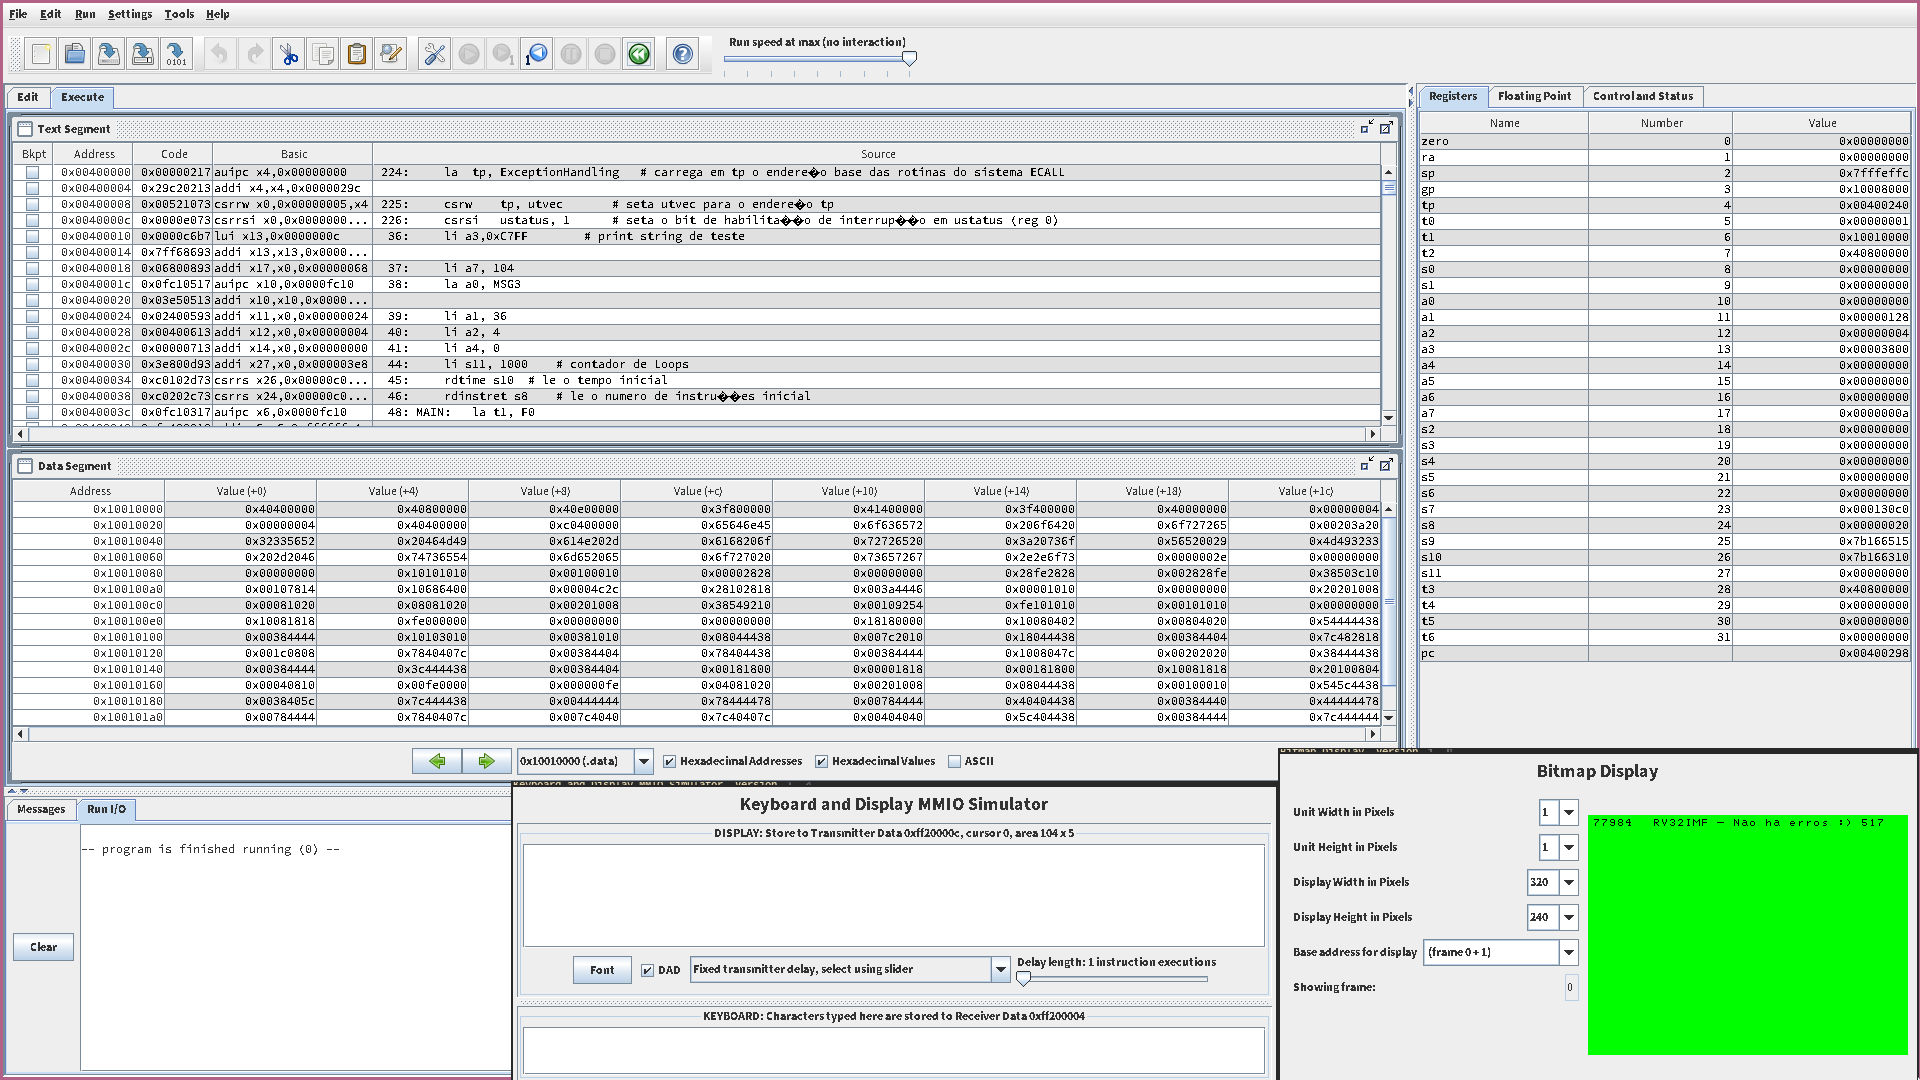
\includegraphics[width=.9\linewidth]{../images/rars_debug.png}
        \caption{Exibição do \textit{frame} de vídeo da \textit{FPGA}}
        \label{fig:rars_debug}
    \end{figure}

    { O \textit{RARS} também é usado para gerar os arquivos \texttt{.mif} para
        inicializar a memória da \textit{FPGA} clicando no menu \texttt{File > Dump Memory}
        ou usando o atalho de teclado \texttt{Ctrl+d}. São gerados dois arquivos,
        um contendo a memória de dados e o outro a memória de texto.
    }

    { Os arquivos \texttt{core/default\_data.mif} e \texttt{core/default\_text.mif}
        são os arquivos gravados na memória da \textit{FPGA} quando é realizada a
        síntese do processador. Esses arquivos também podem ser alterados a tempo
        de execução usando a ferramenta \texttt{Tools > In-System Memory Content
        Editor} do \textit{Quartus}. A pasta \texttt{test/assembly\_testbenches}
        possui alguns programas em \textit{assembly} para testar a \textit{FPGA}.
        Já na pasta \texttt{test/mif\_library}, existem testes já montados prontos
        para gravação na placa de desenvolvimento.
    }

    \section{Interface de vídeo e depuração}
    { A interface de vídeo possui resolução de 320x240 \textit{pixels} com 8
        \textit{bits} de cor para cada pixel. Efetivamente, a interface de vídeo
        possui 255 cores diferentes e uma cor utilizada como transparência, o
        magenta \texttt{0xC7}. Ela também conta com dois \textit{framebuffers},
        permitindo renderizar duas imagens diferentes e alternar entre elas, ou
        se aplicado em um jogo, permite a transição de \textit{frames} sem
        \textit{flickering}: enquanto um \textit{frame} é exibido, o outro
        \textit{framebuffer} é construído com as imagens do próximo \textit{frame},
        e quando pronto, a tela é atualizada com o novo \textit{frame}
        completamente renderizado.
    }

    { A conexão do vídeo do sistema é feita por interface VGA, podendo se
        conectar a qualquer monitor com entrada VGA. A resolução real da
        interface é de 640x480 \textit{pixels} com taxa de atualização de 59 Hz
        por questões de compatibilidade com os monitores. Cada \textit{pixel}
        da interface de vídeo representa uma célula de 4 \textit{pixels} na
        saída de vídeo real. A saída de vídeo VGA também possui 24 \textit{bits}
        de cor, pois o controlador faz a conversão das cores em 8 \textit{bits}
        para três canais de 8 \textit{bits}, um verde, um vermelho e um azul.
    }
    \begin{figure}[H]
    \centering
        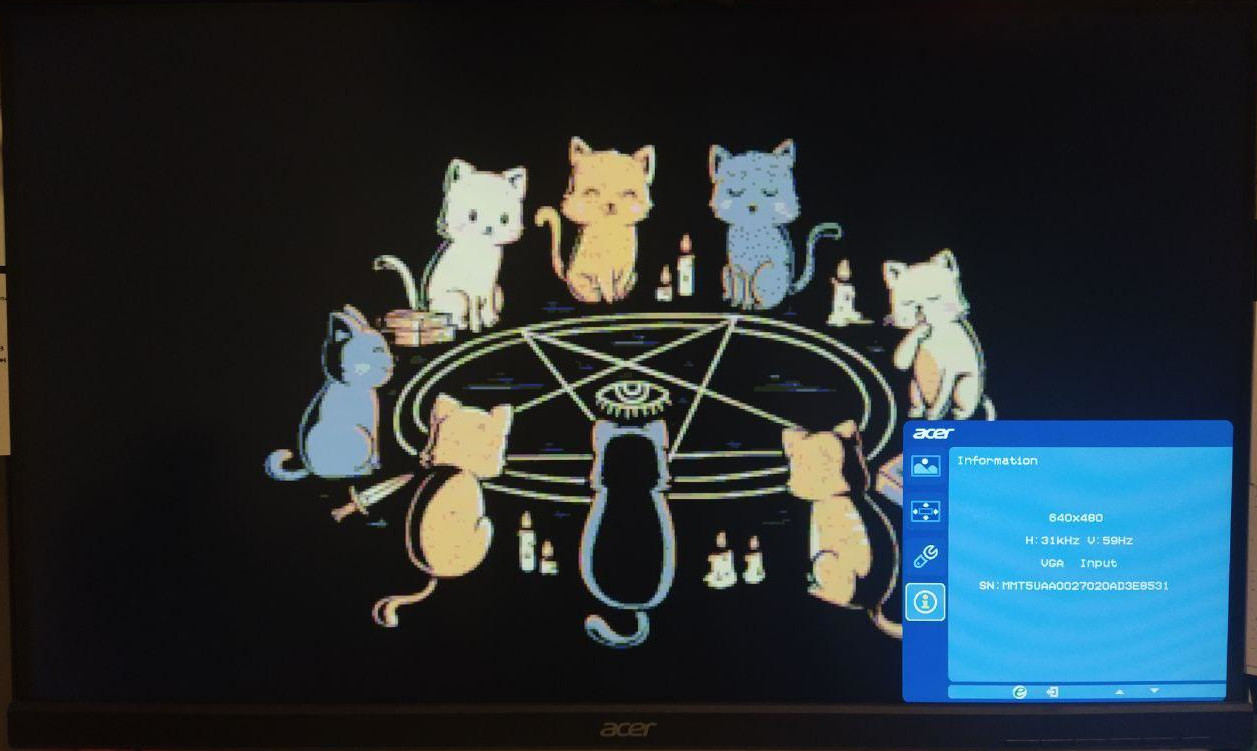
\includegraphics[width=.9\linewidth]{../images/osd/display.jpg}
        \caption{Exibição do \textit{frame} de vídeo da \textit{FPGA}}
        \label{fig:display_cats}
    \end{figure}

    { Acionando um \textit{switch} da \textit{FPGA}, é mostrado por cima do
        \textit{frame} um \textit{menu On Screen Display} que mostra o valor
        atual contido nos bancos de registradores do processador, incluindo os
        \textit{CSRs} e, caso a extensão F esteja implementada, outro
        \textit{switch} permite alternar entre a visualização dos registradores
        de ponto flutuante e os de ponto fixo.
    }
    \begin{figure}[H]
    \centering
        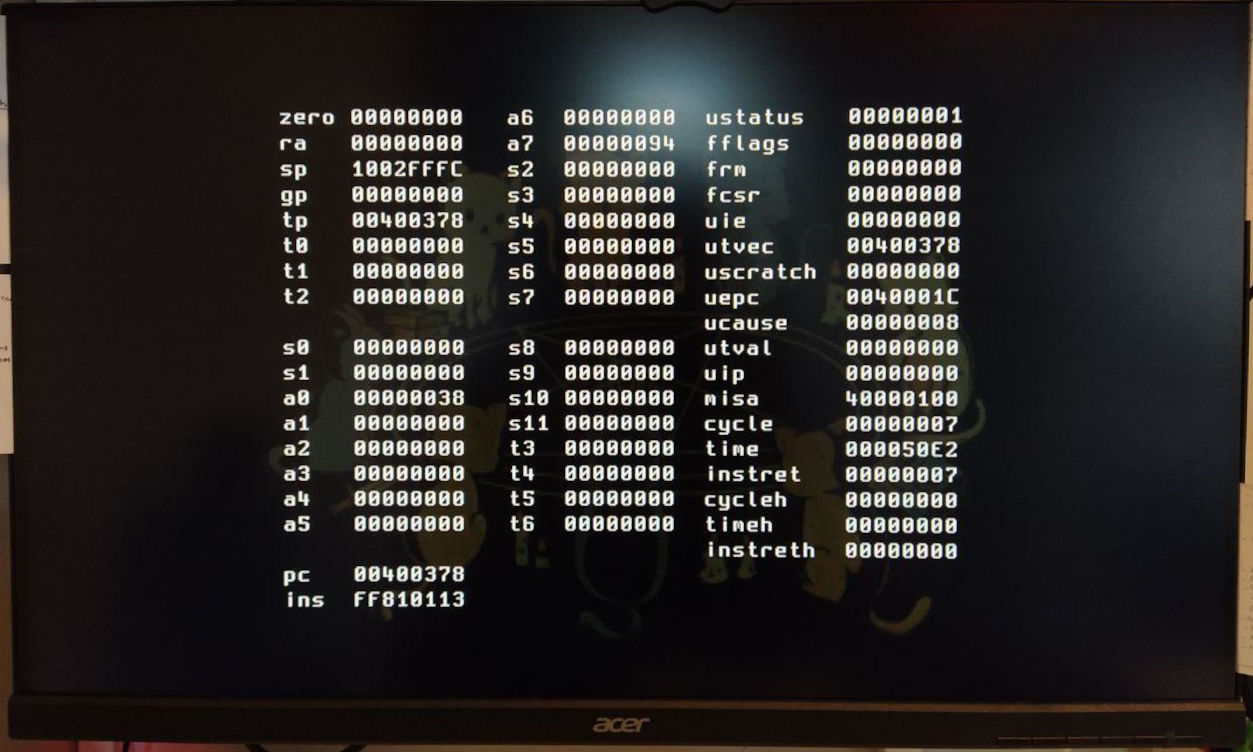
\includegraphics[width=.9\linewidth]{../images/osd/display_osd.jpg}
        \caption{\textit{Menu OSD} exibindo os valores dos registradores do processador}
        \label{fig:display_cats_osd}
    \end{figure}

    { O \textit{menu OSD} é implementado como uma matriz de 52x24 caracteres
        monoespaçados. Na matriz, os caracteres que não mudam com o tempo, como
        é o caso do nome dos registradores, são representados por um parâmetro
        correspondente ao próprio caracter. Já os valores que se alteram, como
        o valor dos registradores, são representados por um parâmetro
        \textit{placeholder}, e o valor a ser mostrado na tela é obtido usando
        uma tabela de \textit{lookup}. O projeto do \textit{menu OSD} foi pensado
        de forma que possa ser modificado para expansão ou utilização em outras
        arquiteturas de processadores de maneira simples.
    }

\section{Configuração e síntese do processador pelo Quartus}
    { O \textit{software} utilizado para a síntese do processador, fornecimento
        de \textit{IPs} como as de memória e operações de ponto flutuante,
        gravação do \textit{soft-core}, dentre outras funcionalidades é o
        \textit{Intel Quartus Lite v18.1}. Versões superiores são compatíveis com
        menos sistemas operacionais e/ou não possuem todos os \textit{IPs}
        necessários para a síntese do processador.
    }
    \begin{figure}[H]
    \centering
        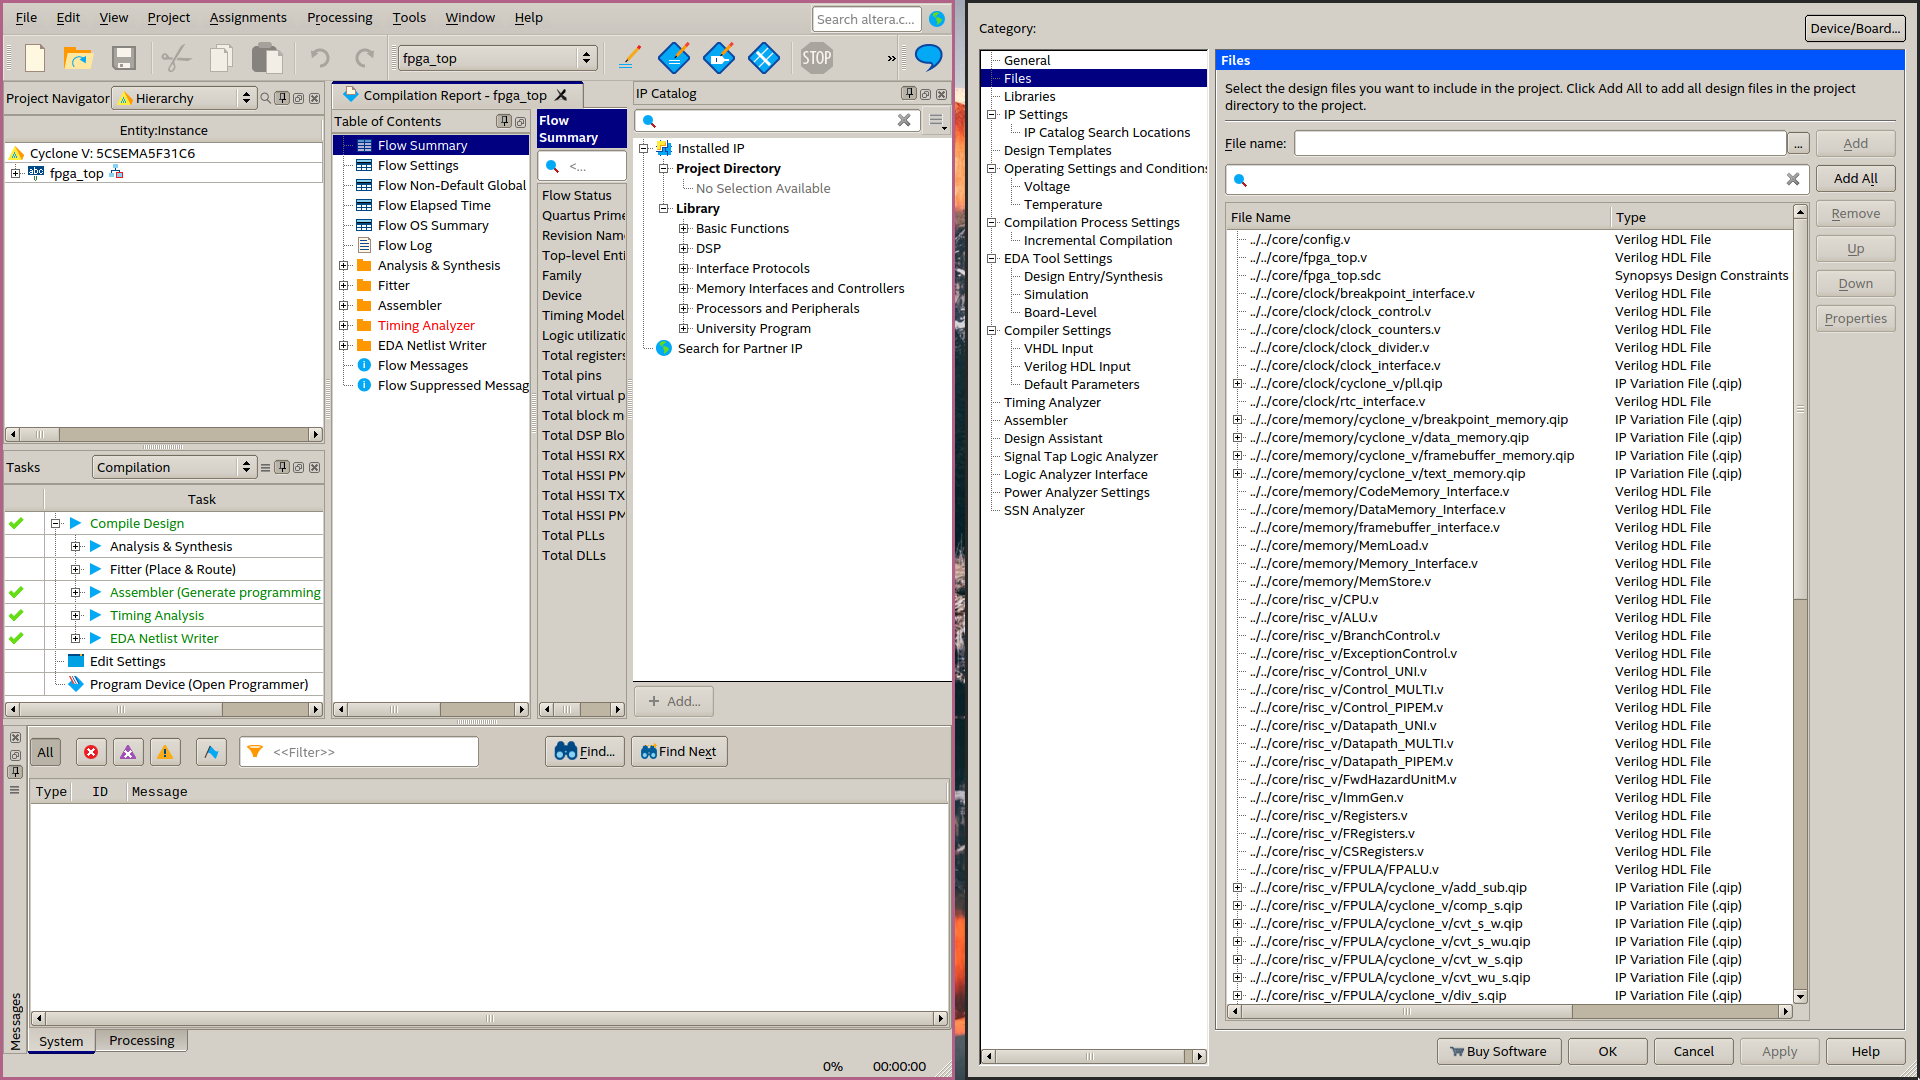
\includegraphics[width=.9\linewidth]{../images/quartus/files_config.png}
        \caption{\textit{Intel Quartus Lite v18.1} com a janela de configurações
            do projeto}\label{fig:quartus_files_config}
    \end{figure}

    { Todas as configurações do projeto também podem ser alteradas manualmente
        no arquivo \texttt{project/de1\_soc/fpga\_top.qsf}. Para ativar ou desativar
        os pinos do \textit{chip} da \textit{FPGA} que conectam os periféricos
        da placa, é preferível que a edição seja feita diretamente no arquivo
        de configuração, comentando ou descomentando a declaração dos pinos.
    }

    { Para realizar a síntese completa do processador para utilizá-lo na \textit{FPGA},
        basta acessar o menu \texttt{Processing > Start Compilation} ou utilizar
        o atalho \texttt{Ctrl + L} ou clicar no ícone de \textit{"Play"}
        na barra de tarefas do programa. Assim, as etapas de Análise e Síntese,
        \textit{Placing} e \textit{Routing}, \textit{Assembler} e
        \textit{Timing Analysis} serão realizadas, e, caso não ocorram erros
        durante o processo, o \textit{soft-core} estará pronto para ser
        gravado na \textit{FPGA} utilizando o arquivo \textit{.mif} gerado.
    }


\section{Simulação do processador pelo Quartus e ModelSim}
    { O projeto possui um \textit{testbench} em \textit{Verilog} para simular as
        entradas e saídas da \textit{FPGA} que o usuário operaria, como os botões
        e \textit{switches}. Ele configura a rotina de reinicialização da placa
        após o \textit{power-up} e define por quanto tempo a simulação será
        executada.
    }

    { O \textit{script} \texttt{test/simulation\_scripts/de1\_soc\_rtl.do} é
        necessário para realizar a simulação de forma correta. O \textit{script}
        gerado automaticamente pelo \textit{Quartus} apresenta problemas que
        impedem que a simulação seja executada corretamente, além de não gerar
        o arquivo de saída da simulação no formato desejado.
    }
    \begin{figure}[H]
    \centering
        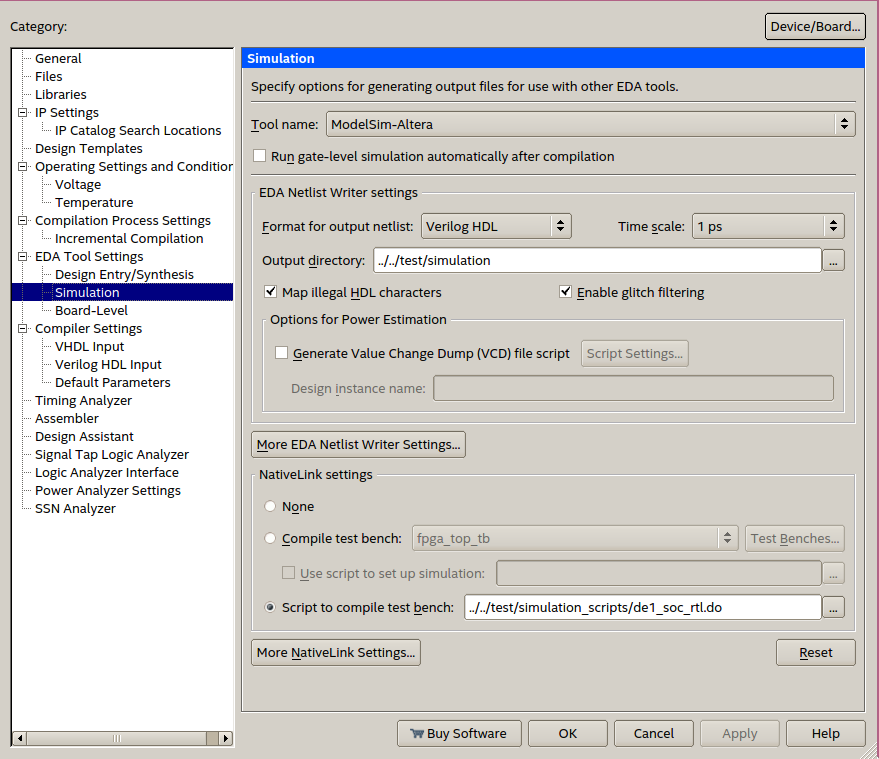
\includegraphics[width=.6\linewidth]{../images/quartus/simulation_config.png}
        \caption{Janela de configuração da simulação no \textit{Quartus}.}
        \label{fig:quartus_simulation_config}
    \end{figure}

    \begin{figure}[H]
    \centering
        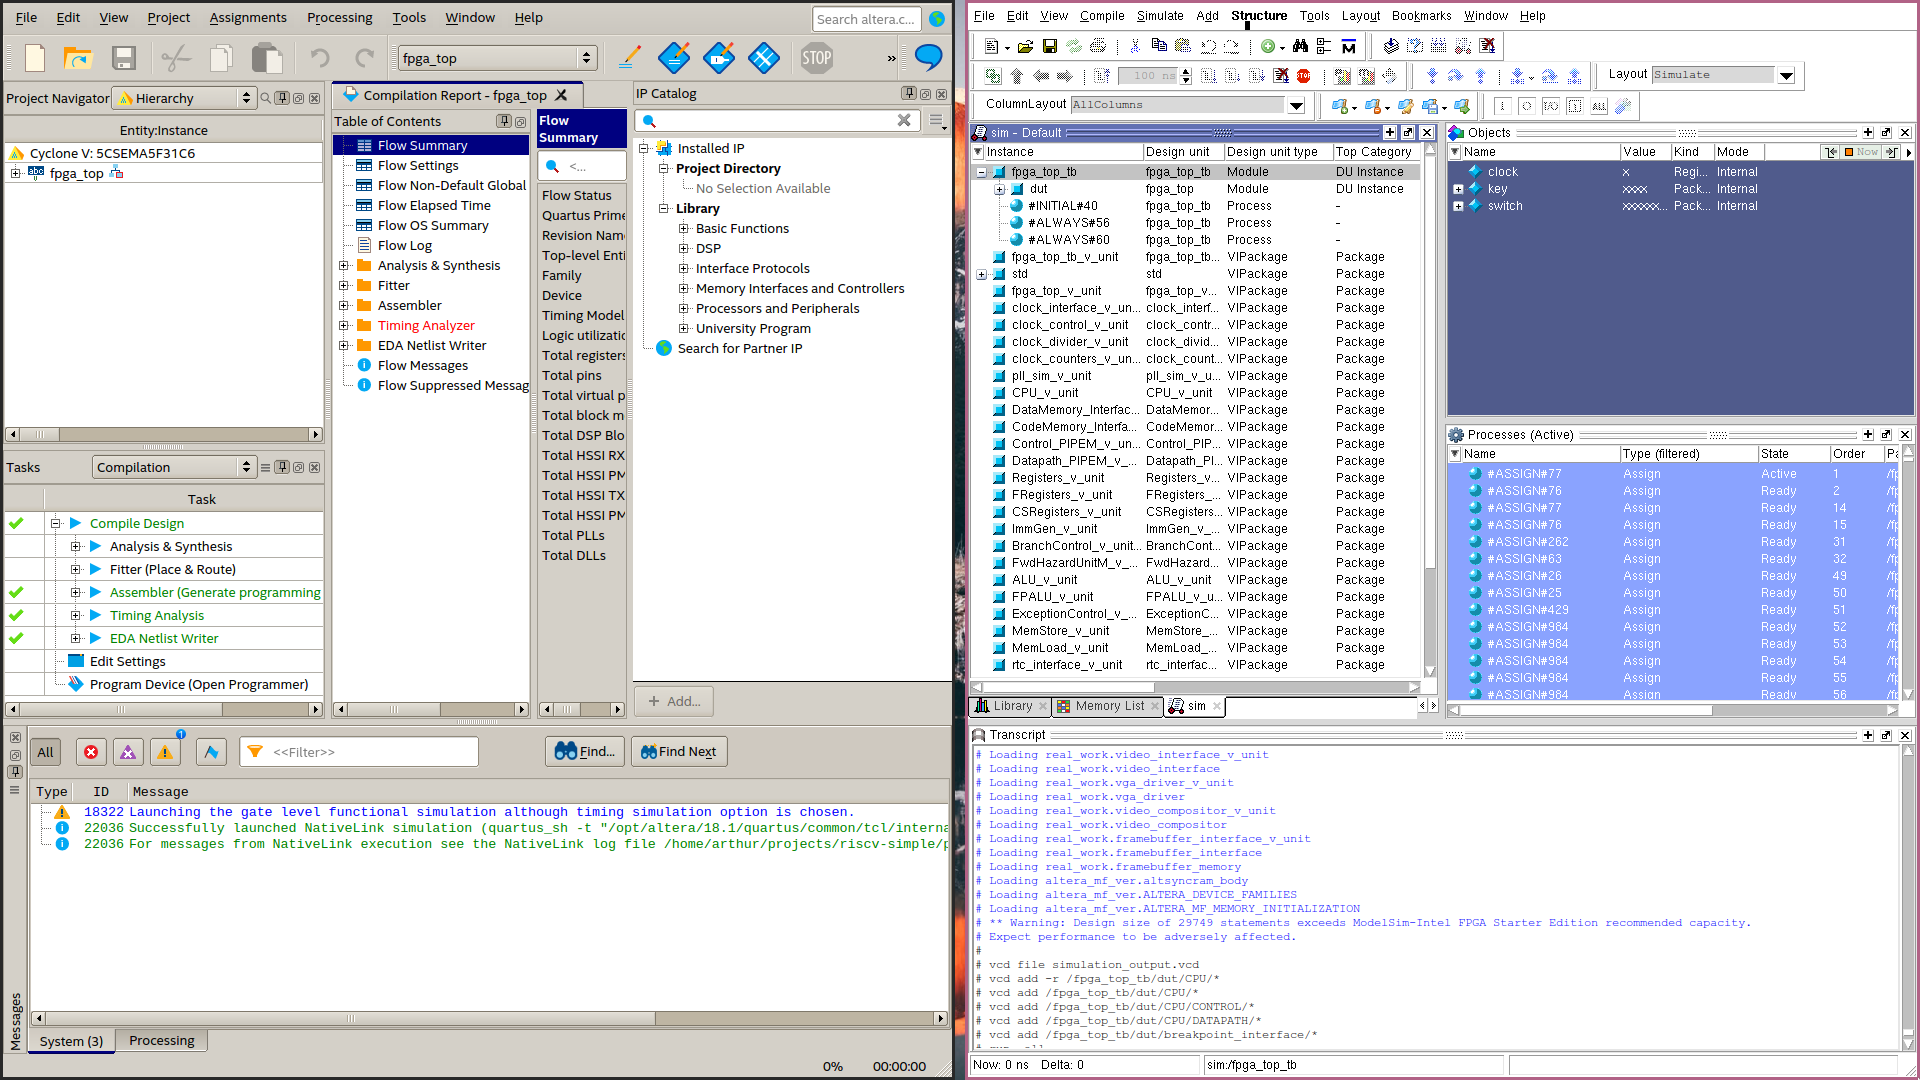
\includegraphics[width=.6\linewidth]{../images/quartus/quartus_modelsim.png}
        \caption{O \textit{script NativeLink} invoca o \textit{ModelSim} passando
            o \textit{script .do} com as informações de como simular o sistema}
        \label{fig:quartus_modelsim}
    \end{figure}

    { Por limitações do \textit{Quartus}, não é possível simular
        \textit{FPGAs Cyclone V} a nível de portas lógicas, somente sendo possível
        fazer a simulação \textit{RTL}. Por outras limitações no programa, o
        \textit{script .do} produzido manualmente só é executado usando o
        \textit{menu} \texttt{Tools > Run Simulation Tool > Gate Level Simulation},
        que, apesar do nome, executará uma simulação \textit{RTL}. A opção
        \texttt{Tools > Run Simulation Tool > RTL Simulation} utiliza o \textit{script}
        .do gerado automaticamente, e falha ao ser processado.
    }

    { Ao executar a simulação, os \textit{scripts NativeLink} iniciarão o
        programa \textit{ModelSim}, carregando o \textit{script .do} customizado,
        conforme mostrado na Figura~\ref{fig:quartus_modelsim}. Ao finalizar a
        simulação, um arquivo \texttt{.vcd} será gerado e poderá ser analisado
        em \textit{softwares} de visualização de formatos de onda, como o
        \textit{GTKWave} ou o próprio \textit{ModelSim}.
    }

    { Ao carregar um arquivo \texttt{.vcd} no \textit{GTKWave}, a hierarquia
        dos módulos é mostrada em uma árvore no canto superior esquerdo da tela.
        Ao clicar no nó desejado da árvore, os sinais do módulo serão mostrados
        no canto inferior esquerdo da tela. Para visualizá-lo, basta clicar e
        arrastar o sinal para a área \textit{Signals}. A Figura~\ref{fig:gtkwave_generic}
        mostra uma visualização dos sinais escolhidos. Na pasta \texttt{test/gtkwave}
        do projeto, existe um arquivo \texttt{.gtkw} para cada uma das nove
        configurações do \textit{soft-core} com sinais predefinidos.
    }

    \begin{figure}[H]
    \centering
        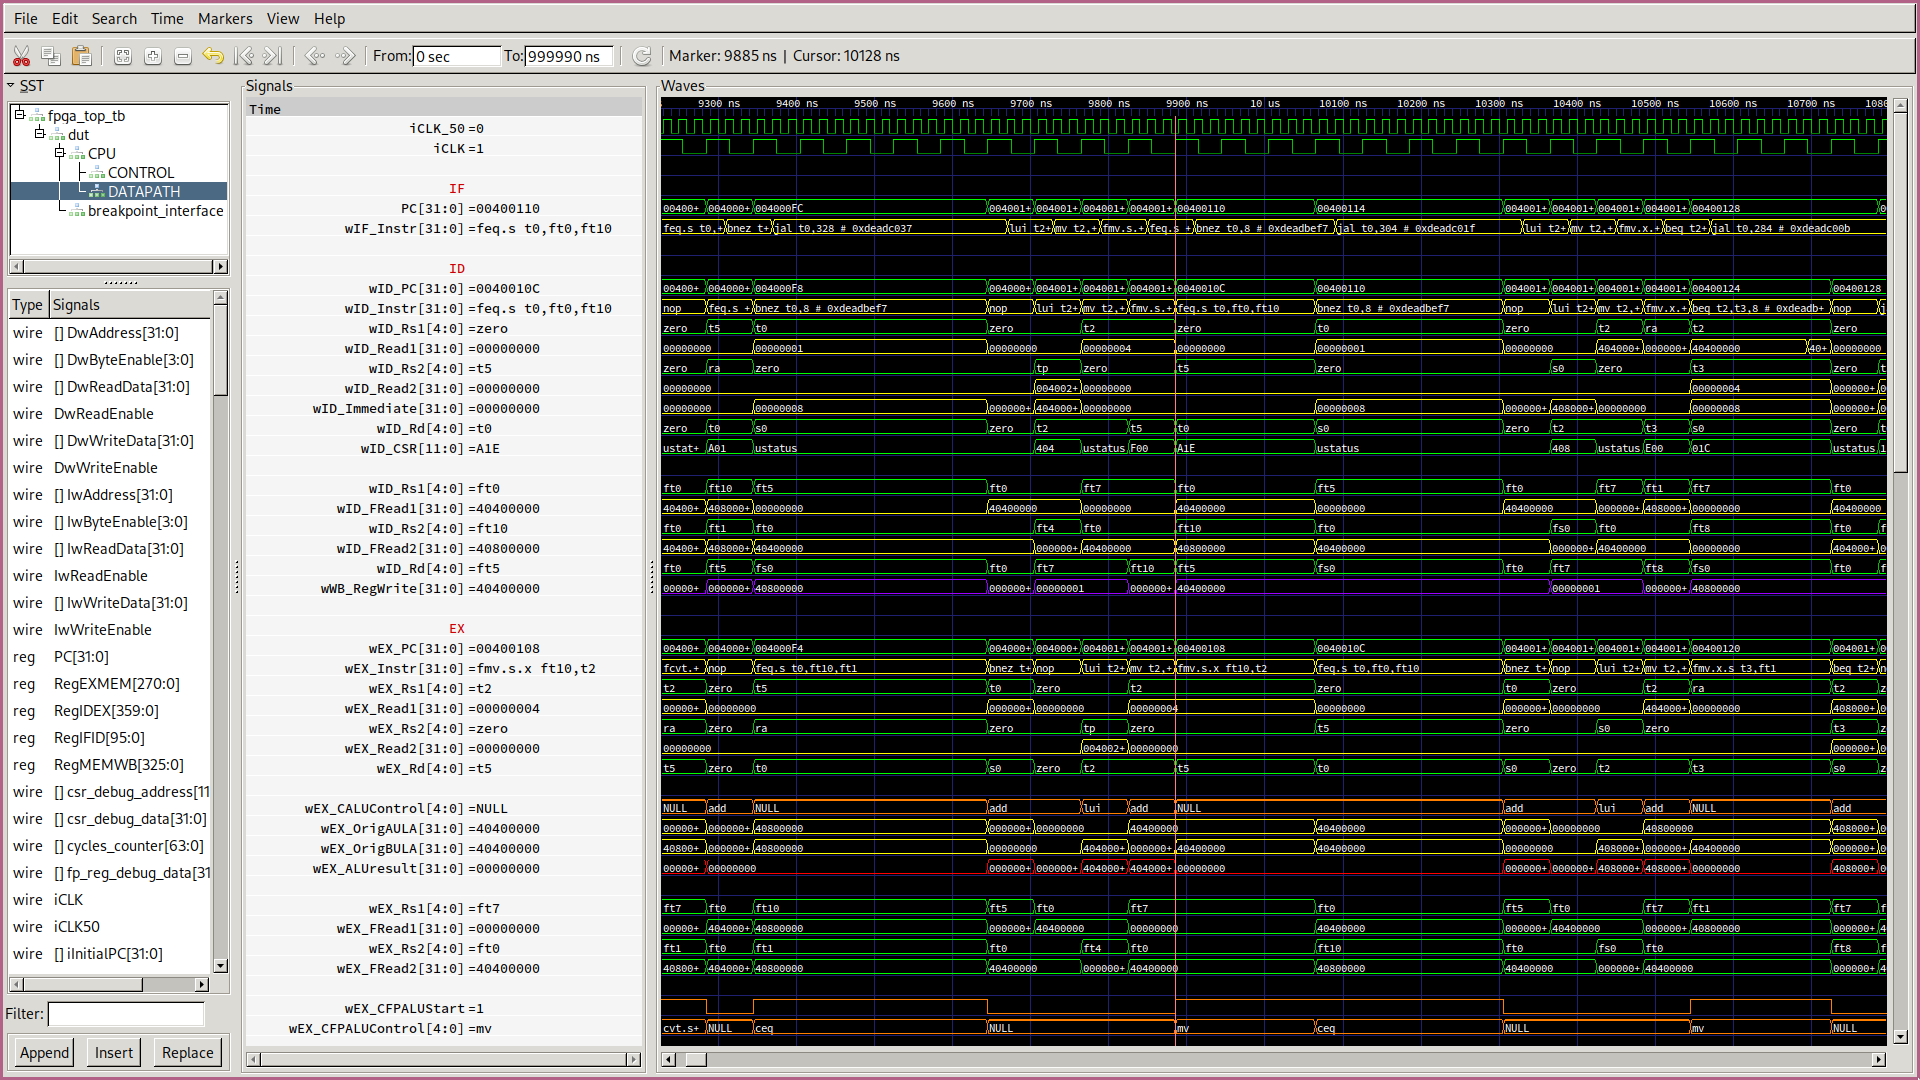
\includegraphics[width=.9\linewidth]{../images/gtkwave/random.png}
        \caption{Visualização das formas de onda no GTKWave}
        \label{fig:gtkwave_generic}
    \end{figure}

    { É possível escolher as cores dos sinais para melhor destaque, bem como
        utilizar arquivos e programas para a tradução de valores dos sinais.
        Na pasta \texttt{test/gtkwave/translation\_files} se encontram arquivos
        \texttt{.txt} para tradução dos códigos hexadecimais dos seletores de
        registradores e de controle das unidades de lógica e aritmética. Assim,
        a visualização da forma de onda mostra os mnemônicos dos sinais, facilitando
        sua compreensão. O programa \texttt{riscv-decode} presente em
        \texttt{tools/riscv-disassembler/build} desmonta as instruções e as exibe
        na visualização.
    }


\section{Script \texttt{make.sh}}
    { A pasta \texttt{test/sof\_library} contém os arquivos \texttt{.sof} com
        as nove variações da última versão do processador, prontos para serem
        gravados na \textit{FPGA}. Para facilitar a geração das nove variantes,
        o \textit{bash script} \texttt{make.sh} foi criado para automatizar a
        síntese, salvando as novas versões na pasta \texttt{test/sof\_library}.
        O \textit{script} também permite realizar somente a etapa de
        análise das variantes para confirmar que alterações feitas no código não
        introduziram erros de compilação, uma vez que é um processo muito mais
        ágil que realizar a síntese completa.
    }

    { Além disso, o \textit{script} também possui opção para simular \textit{RTL}
        todas as variantes do processador, salvando os \textit{logs} e arquivos
        \textit{.vcd} na pasta \texttt{test/simulation}. A pasta \texttt{test/simulation}
        é ignorada pelo \textit{git}, pois os arquivos de forma de onda podem
        ficar grandes demais a ponto de inviabilizar seu versionamento.
    }

    \section{Uso da FPGA DE1-SoC}
    { A placa de desenvolvimento \textit{terasIC DE1-SoC} utilizada no projeto
        é mostrada na Figura~\ref{fig:de1_soc}.
    }

    { Os botões e \textit{switches} mostrados na Figura~\ref{fig:de1_soc} são
        utilizados para controlar as características do \textit{clock} do
        processador, fazer seu \textit{reset} e controlar o \textit{menu OSD}
        de depuração. A função de cada \textit{input} é:
    }
    \begin{itemize}
        \setlength\itemsep{0em}
        \item \texttt{KEY0}: Reset do processador;
        \item \texttt{KEY1}: Seletor de divisor de \textit{clock} lento ou rápido;
        \item \texttt{KEY2}: Seletor de \textit{clock} manual ou automático;
        \item \texttt{KEY3}: Gerador de \textit{clock} manual;
        \item \texttt{SW0}: Bit [0] do divisor de \textit{clock};
        \item \texttt{SW1}: Bit [1] do divisor de \textit{clock};
        \item \texttt{SW2}: Bit [2] do divisor de \textit{clock};
        \item \texttt{SW3}: Bit [3] do divisor de \textit{clock};
        \item \texttt{SW4}: Bit [4] do divisor de \textit{clock};
        \item \texttt{SW5}: Temporizador para \textit{stall} do processador;
        \item \texttt{SW6}: Seletor de \textit{framebuffer} a ser exibido;
        \item \texttt{SW7}: Seletor de banco de registradores no \textit{menu OSD};
        \item \texttt{SW8}: Sem função;
        \item \texttt{SW9}: Habilita o \textit{menu OSD};
    \end{itemize}

    \begin{figure}[H]
    \centering
        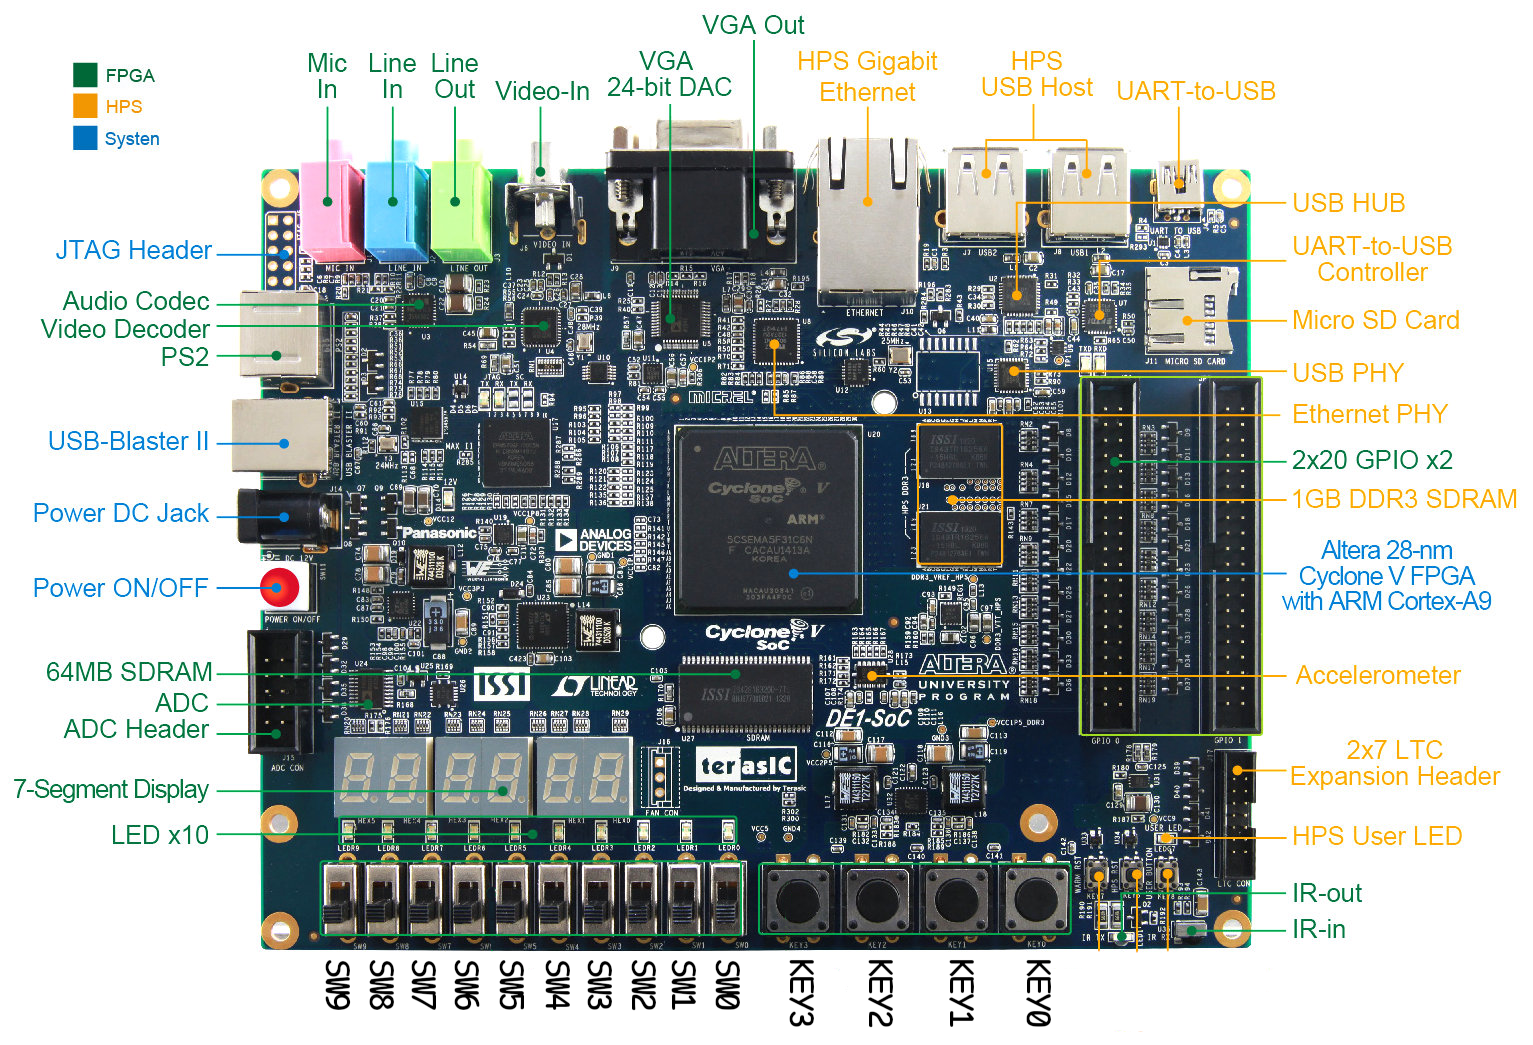
\includegraphics[width=.9\linewidth]{../images/fpga/de1_soc_subs.png}
        \caption[Placa de desenvolvimento \textit{terasIC DE1-SoC}.]{Placa de
        desenvolvimento \textit{terasIC DE1-SoC}.\quad Fonte:~\cite{terasic_de1_soc}}
        \label{fig:de1_soc}
    \end{figure}

    { O procedimento recomendado para inicialização do processador após o
        \textit{Programmer} do \textit{Quartus} programar a \textit{FPGA} com
        um novo arquivo \textit{.mif} é: Pressionar e soltar a \texttt{KEY2}
        para ativar o \textit{clock} automático; pressionar e soltar a
        \texttt{KEY0} para dar o \textit{reset} dos estados do processador e,
        caso queira uma execução mais rápida, pressionar e soltar a \texttt{KEY1}
        para mudar para um divisor de \textit{clock} mais veloz. A frequência
        máxima de operação do \textit{clock} é de 50MHz, e ocorre na opção de
        divisor rápido com o divisor \texttt{5'b1}.
    }

    { Utilizando a saída de vídeo, o sistema pode executar programas gráficos
        como jogos, ou pode ser usado simplesmente como ferramenta de \textit{debug}.
        Ativando o \textit{menu OSD} e utilizando o \textit{clock} manual, é
        possível ver a progressão dos registradores do processador instrução por
        instrução.
    }

    { O processador também pode receber \textit{inputs} do usuário utilizando
        um teclado \textit{PS/2}. A leitura do teclado é realizada por meio de
        \textit{polling} do endereço do \textit{buffer} do teclado.
    }

%     { A interface \textit{RS-232} também pode ser utilizada para enviar e receber
%         dados provenientes de outro computador, permitindo contornar a limitação
%         de pouca memória disponível na \textit{FPGA}, enviando novos dados e
%         instruções à medida em que forem necessários e/ou requisitados pelo
%         processador.
%     }


\section{Observações Finais do Sistema Proposto}
    { No presente capítulo vimos o detalhamento da implementação e das ferramentas
        utilizadas no ambiente de aprendizado, e como utilizá-las. No próximo
        capítulo, trataremos dos resultados do trabalho, apresentando tabelas
        comparativas entre as implementações, análise de performance e visualizações
        das formas de onda do sistema simulado.
    }


\chapter{Resultados}\label{cap4_resultados}

{ Após a exposição dos componentes do ambiente de aprendizado e estrutura das
    implementações do processador, é possível realizar análises quantitativas
    e qualitativas dos resultados obtidos.
}

{ As seções desse capítulo explorarão os resultados da síntese e simulação de
    cada versão, além de apresentar resultados de \textit{benchmarks} sintéticos
    a fim de comparar o desempenho de cada implementação e sua viabilidade de uso.
}

{ O código-fonte e demais arquivos da plataforma \textit{RISC-V SiMPLE} denvolvida
    está disponível no \textit{link} \url{https://github.com/LAICO-UnB/riscv-simple}
    com licença \textit{open-source BSD 3-Clause}. O código-fonte e \texttt{.pdf}
    dessa monografia está disponível no \textit{link} \url{https://github.com/arthurbeggs/monografia}
    com licença \textit{open-source BSD 3-Clause}.
}

\section{Síntese dos \textit{soft-cores}}
    { As nove diferentes implementações do processador foram geradas usando o \textit{script}
        \texttt{./make.sh \--simulate}, produzindo os arquivos \texttt{.sof} para
        gravação na \textit{FPGA}, os \texttt{.vcd} de simulação em forma de onda
        e os \texttt{.rpt} de resumo do \textit{Quartus}.
    }

    { Os dados da Tabela~\ref{table:synth_resources} foram obtidos dos arquivos
        \texttt{.rpt} e executando os arquivos \texttt{.sof} na placa \textit{DE1-SoC}.
        Cada \textit{ISA} foi carregada com um \textit{benchmark} específico para seu
        conjunto de instruções. Os códigos-fonte podem ser encontrados em
        \texttt{test/assembly\_testbench} e suas versões montadas estão disponíveis
        na pasta \texttt{test/mif\_library}.
    }

    \begin{longtable}{cc|c|c|c|c|c|c|c|}
        \caption{Características dos sistemas implementados}\label{table:synth_resources}\\
        \cline{3-9}
                                                                &                               & ALMs  & Regs  & Pins  & Mem Bits  & DSPs  & PLLs  & Max Clk   \\
        \cline{2-9}
                                                                & \multicolumn{1}{|c|}{Máximo}  & 32070 & XXXXX & 457   & 4065280   & 87    & 1     & 50MHz     \\
        \hline
        \endfirsthead
        \cline{3-9}
                                                                &                               & ALMs  & Regs  & Pins  & Mem Bits  & DSPs  & PLLs  & Max Clk   \\
        \cline{2-9}
                                                                & \multicolumn{1}{|c|}{Máximo}  & 32070 & XXXXX & 457   & 4065280   & 87    & 1     & 50MHz     \\
        \hline
        \endhead
        \multicolumn{1}{|c}{\multirow{3}{*}{{Uniciclo}}}        & \multicolumn{1}{|c|}{RV32I}   & 4123  & 3160  & 103   & 2805792   & 0     & 1     & 12.5MHz   \\*
        \cline{2-9}
        \multicolumn{1}{|c}{ }                                  & \multicolumn{1}{|c|}{RV32IM}  & 7047  & 3179  & 103   & 2805792   & 12    & 1     & 12.5MHz   \\*
        \cline{2-9}
        \multicolumn{1}{|c}{ }                                  & \multicolumn{1}{|c|}{RV32IMF} & 9411  & 5558  & 103   & 2853408   & 18    & 1     & 4.17Mhz   \\
        \hline
        \multicolumn{1}{|c}{\multirow{3}{*}{{Multiciclo}}}      & \multicolumn{1}{|c|}{RV32I}   & 4102  & 3444  & 103   & 2805792   & 0     & 1     & 25MHz     \\*
        \cline{2-9}
        \multicolumn{1}{|c}{ }                                  & \multicolumn{1}{|c|}{RV32IM}  & 6726  & 3471  & 103   & 2805792   & 12    & 1     & 25MHz     \\*
        \cline{2-9}
        \multicolumn{1}{|c}{ }                                  & \multicolumn{1}{|c|}{RV32IMF} & 9108  & 5737  & 103   & 2853408   & 18    & 1     & 25MHz     \\
        \hline
        \multicolumn{1}{|c}{\multirow{3}{*}{\textit{Pipeline}}} & \multicolumn{1}{|c|}{RV32I}   & 4605  & 4139  & 103   & 2805792   & 0     & 1     & 50MHz     \\*
        \cline{2-9}
        \multicolumn{1}{|c}{ }                                  & \multicolumn{1}{|c|}{RV32IM}  & 7376  & 4145  & 103   & 2805792   & 12    & 1     & 25MHz     \\*
        \cline{2-9}
        \multicolumn{1}{|c}{ }                                  & \multicolumn{1}{|c|}{RV32IMF} & 9750  & 6568  & 103   & 2853408   & 18    & 1     & 25MHz*    \\
        \hline
    \end{longtable}

    { Ao analisar a tabela, podemos tirar as seguintes conclusões: }
    \begin{itemize}
        \item   O número de \textit{PLLs} e de pinos não muda entre as implementações,
            pois somente um \textit{PLL} é utilizado para gerar os sinais de relógio da
            \textit{FPGA}, e o \textit{pinout} do módulo \textit{top level} não é alterado
            entre as versões do processador. Variação nesses valores representaria um erro;
        \item   O número de \textit{DSPs} é \texttt{0} para o uniciclo, \texttt{12} para o
            multiciclo e \texttt{18} para o \textit{pipeline}. Os \textit{DSPs} apenas
            são utilizados nas operações de \textit{mul/div} e ponto flutuante;
        \item   A quantia de \textit{bits} de memória utilizados permanece igual para
            todas as implementações do uniciclo e multiciclo. Todas as implementações
            do \textit{pipeline} também utilizam a mesma quantia de \textit{bits}, que
            é levemente maior que nas outras duas microarquiteturas;
        \item   Como é de se esperar, a quantia de \textit{ALMs} e \textit{registradores}
            aumenta ao implementar mais extensões numa mesma microarquitetura;
        \item   A microarquitetura multiciclo utiliza a menor quantia de recursos entre
            as três, resultado esperado já que sua implementação reutiliza estruturas como
            a ULA na sua execução por microcódigo, enquanto as outras arquiteturas utilizam
            mais de um somador com funções específicas em seu \textit{datapath};
        \item   A frequência máxima de operação do multiciclo se manteve constante para as
            três \textit{ISAs} implementadas e teve bom desempenho;
        \item   A frequência de operação do uniciclo foi a mais baixa entre os sistemas
            implementados, como era esperado. Com o uso de operações de ponto flutuante,
            sua frequência máxima foi bastante penalizada;
        \item   A implementação da \textit{ISA RV32IMF} no \textit{pipeline} apresenta
            erros devido a \textit{forwards e hazards} não tratados ou tratados de maneira
            incorreta. Há um ``*'' em sua frequência pois não é possível realizar o teste
            até sua complitude.
    \end{itemize}

\section{Formas de Onda das Simulações}
    { As Figuras \ref{fig:gtkwave_uni}, \ref{fig:gtkwave_multi} e \ref{fig:gtkwave_pipe}
        mostram as visualizações criadas para as simulações dos \textit{soft-cores}
        \textbf{RV32IMF} uniciclo, multiciclo e \textit{pipeline} respectivamente.
        Nelas, as instruções passam por um \textit{desassembler}, os registradores
        são mostrados com seus nomes mnemônicos e os sinais possuem cores diferentes
        dependendo de sua origem.
    }

    { Com essas visualizações, o processo de depuração do processador é facilitado.
        Alguns \textit{bugs} do \textit{pipeline} só puderam ser identificados graças
        à simulação. Os sinais adicionados são suficientes para a maioria das inspeções,
        mas se necessário, novos sinais podem ser adicionados.
    }

    \begin{figure}[H]
    \centering
        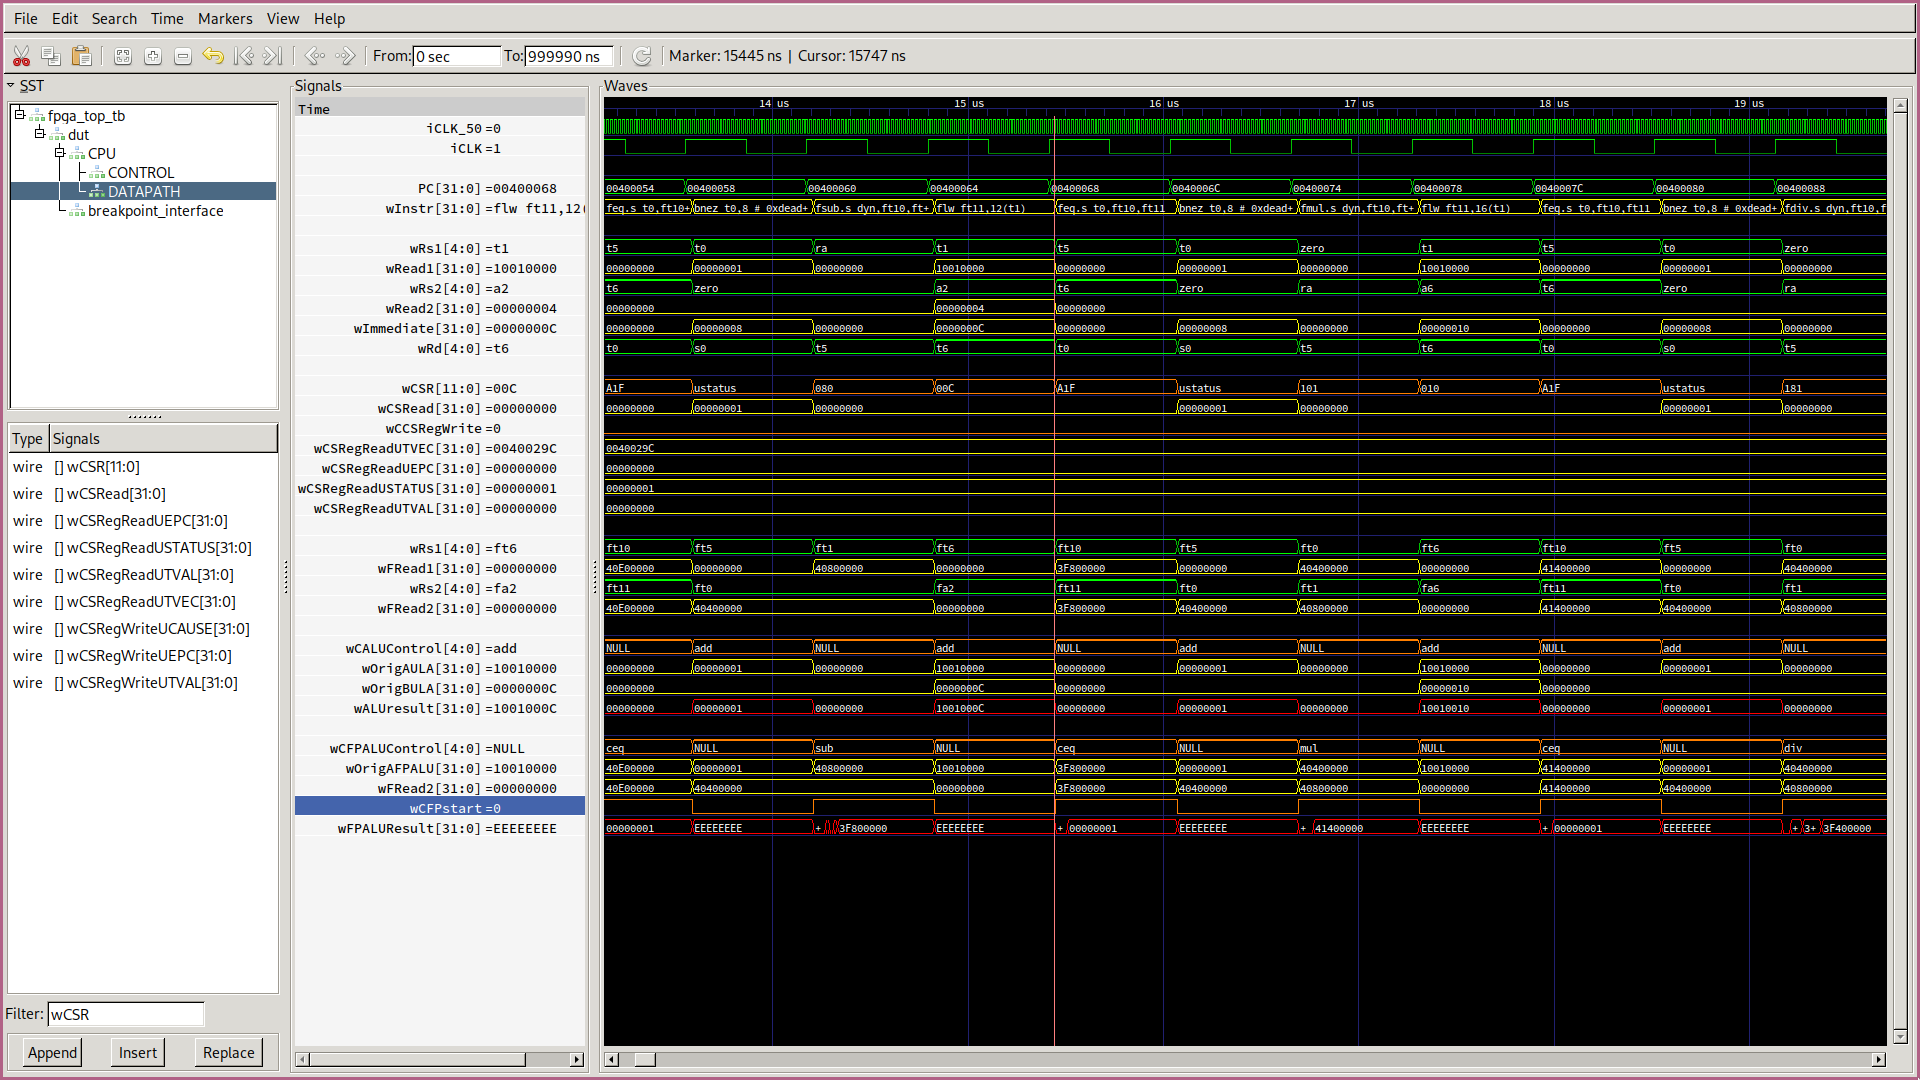
\includegraphics[width=0.9\linewidth]{../images/gtkwave/gtkwave_uni.png}
        \caption{Visualização das formas de onda \textit{soft-core} \textbf{RV32IMF} uniciclo}
        \label{fig:gtkwave_uni}
    \end{figure}

    \begin{figure}[H]
    \centering
        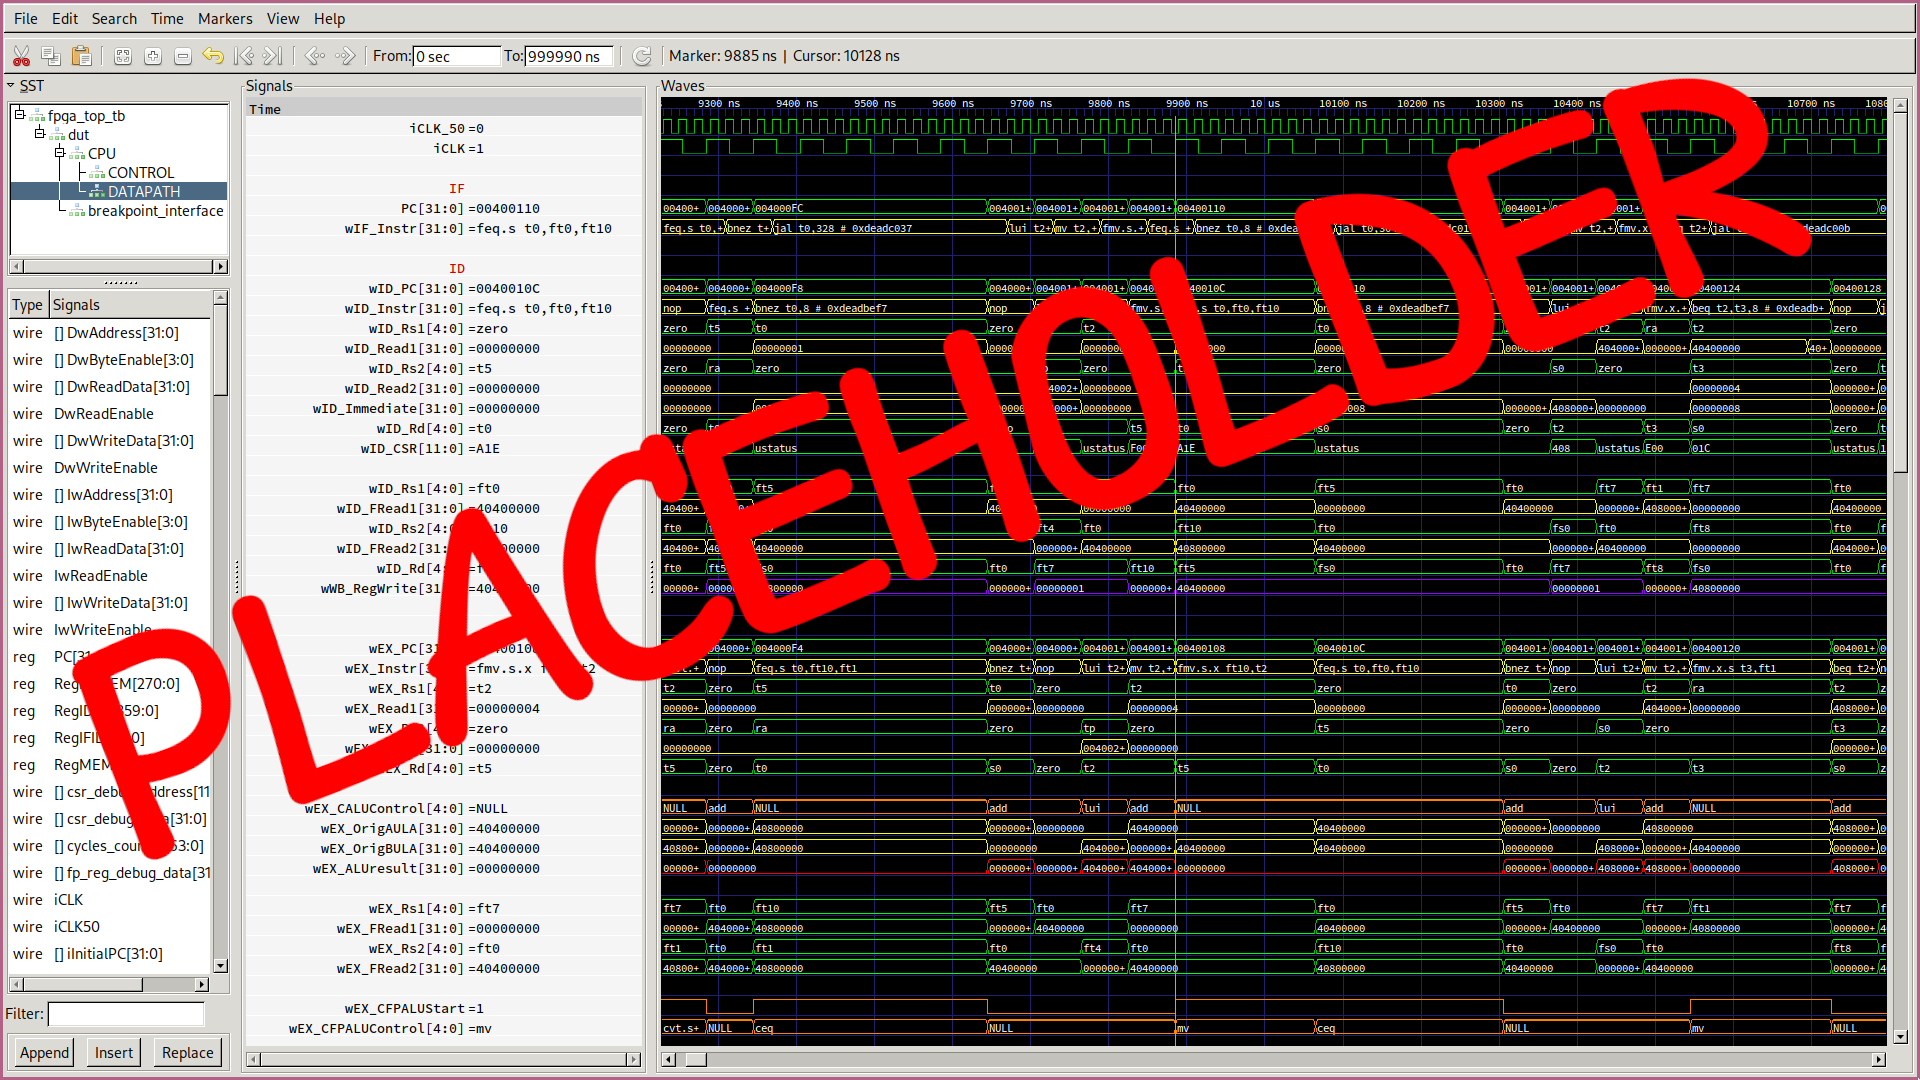
\includegraphics[width=0.9\linewidth]{../images/gtkwave/gtkwave_multi.png}
        \caption{Visualização das formas de onda \textit{soft-core} \textbf{RV32IMF} multiciclo}
        \label{fig:gtkwave_multi}
    \end{figure}

    \begin{figure}[H]
    \centering
        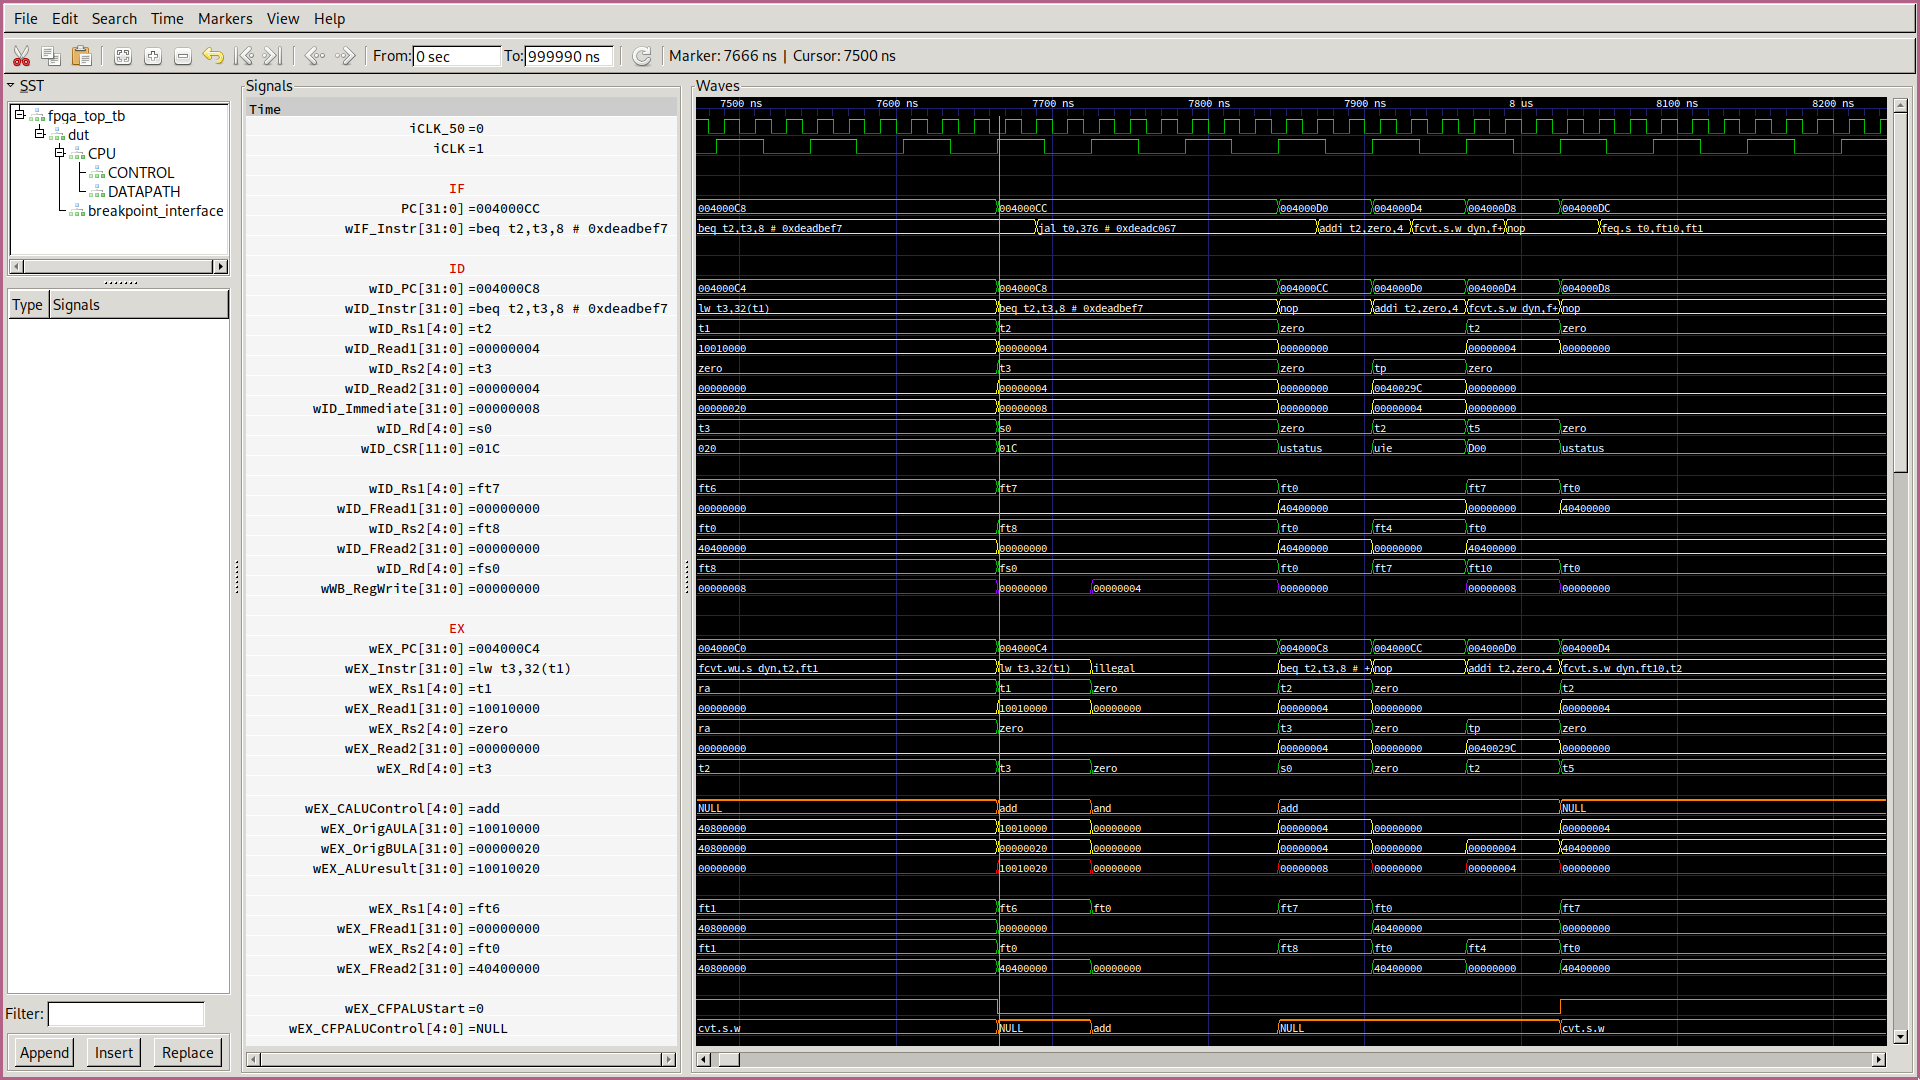
\includegraphics[width=0.9\linewidth]{../images/gtkwave/gtkwave_pipe.png}
        \caption{Visualização das formas de onda \textit{soft-core} \textbf{RV32IMF} \textit{pipeline}}
        \label{fig:gtkwave_pipe}
    \end{figure}

\section{\textit{Benchmarks} (Incompleto)}
    {
    }
    \begin{longtable}{|l|}
        \caption{\textit{Benchmark}}\label{table:benchmark}\\
        \hline
        \hline
        \endfirsthead
        \hline
        \hline
        \endhead
        \hline
    \end{longtable}

\section{Observações Finais dos Resultados (Incompleto)}
    % NOTE: Falar sobre os benchmarks

    { O próximo capítulo encerrará o presente trabalho fazendo observações
        pertinentes aos resultados obtidos, à viabilidade do uso da plataforma
        desenvolvida para os propósitos desejados e perspectivas futuras,
        tratando de possíveis melhorias e expansão do escopo.
    }


\chapter{Conclusões}\label{cap5_conclusoes}


\section{Perspectivas Futuras}

    % NOTE: Colocar em lugar apropriado
    { Com o recente sucesso dos processadores \textit{ARM M1} lançados pela
        \textit{Apple}, e com os processadores \textit{ARM Graviton} disponíveis
        no serviço de servidores em nuvem da \textit{Amazon}, é uma possibilidade
        forte que o desenvolvimento de plataformas \textit{RISC-V} para uso geral
        desacelere.
    }




% % Bibliografia
\renewcommand{\bibname}{REFERÊNCIAS BIBLIOGRÁFICAS}
\addcontentsline{toc}{chapter}{REFERÊNCIAS BIBLIOGRÁFICAS}


\bibliographystyle{abnt-num}
\bibliography{relatorio.bib}

% Anexos
\anexos{}
\makeatletter
\renewcommand{\@makechapterhead}[1]{
  { \parindent\z@ \raggedleft\setfontarial\bfseries
    \LARGE \thechapter. \space\space \uppercase{#1}\par \vskip 40\p@
  }
}
\makeatother

% Anexo I: Descrição do CD

\chapter{Descrição do conteúdo do CD}

\label{AnCD}

Descrever CD.


\refstepcounter{noAnexo}

% Anexo II: Programas Utilizados

\chapter{Programas utilizados}

Quais programas foram utilizados?


\refstepcounter{noAnexo}

\end{document}
